\section{Preliminary studies}

\subsection{Homogeneous vs. heterogeneous isotope distribution}

This section conducted a study to determine the proper way to treat the fuel compact heterogeneities in Serpent.
This study modeled two different isotope distributions in a fuel compact.
First, a homogeneous distribution of the isotopes.
Second, a heterogeneous distribution, in which we explicitly modeled the TRISO particles.
We modeled both cases using Serpent.
We used a hexagonal unit cell model that included the fuel compact, a helium gap, and the surrounding graphite.
Table \ref{tab:compact} specifies the model input parameters.
The material temperature was 1200K, a case that represents the \gls{HFP} core state.
Serpent ran 5$\times 10^4$ neutrons/cycle, 500 active cycles, and 50 inactive cycles for the calculations.
The simulations took 1.73 and 2.21 minutes using 256 cores.
The heterogeneous calculation took 28$\%$ more.

The \gls{Keff} was 1.17523 for the homogeneous distribution and 1.25106 for the heterogeneous distribution.
Using the heterogeneous distribution as a reference, we calculated the relative error of some of the group constants in an eigenvalue calculation.
Serpent generated the group constants using the three energy group structure in Table \ref{tab:energygroups}.
The evaluated parameters were $D_g$, $\Sigma^r_g$, $\nu\Sigma^f_g$, and $\chi^t_g$ (see equation \ref{eq:diffusion}).
Figure \ref{fig:param-comparison} displays the relative errors for $\Sigma^r_g$ (REMXS) and $\nu\Sigma^f_g$ (NSF), which were the group constants that changed the most.
The figure does not include $D_g$ and $\chi^t_g$ because their relative errors were less than 1$\%$.
The relative errors of $\Sigma^r_g$ and $\nu\Sigma^f_g$ were less than 6$\%$.

% \cite{strydom_results_2015}
% The low multiplication factor in the homogeneous case is due to the fuel self-shielding .
% In the heterogeneous compact, the fuel self-shielding leads to a significantly decreased U-238 neutron absorption compared to the homogeneous fuel compact.

\begin{figure}[htbp!]
	\centering
	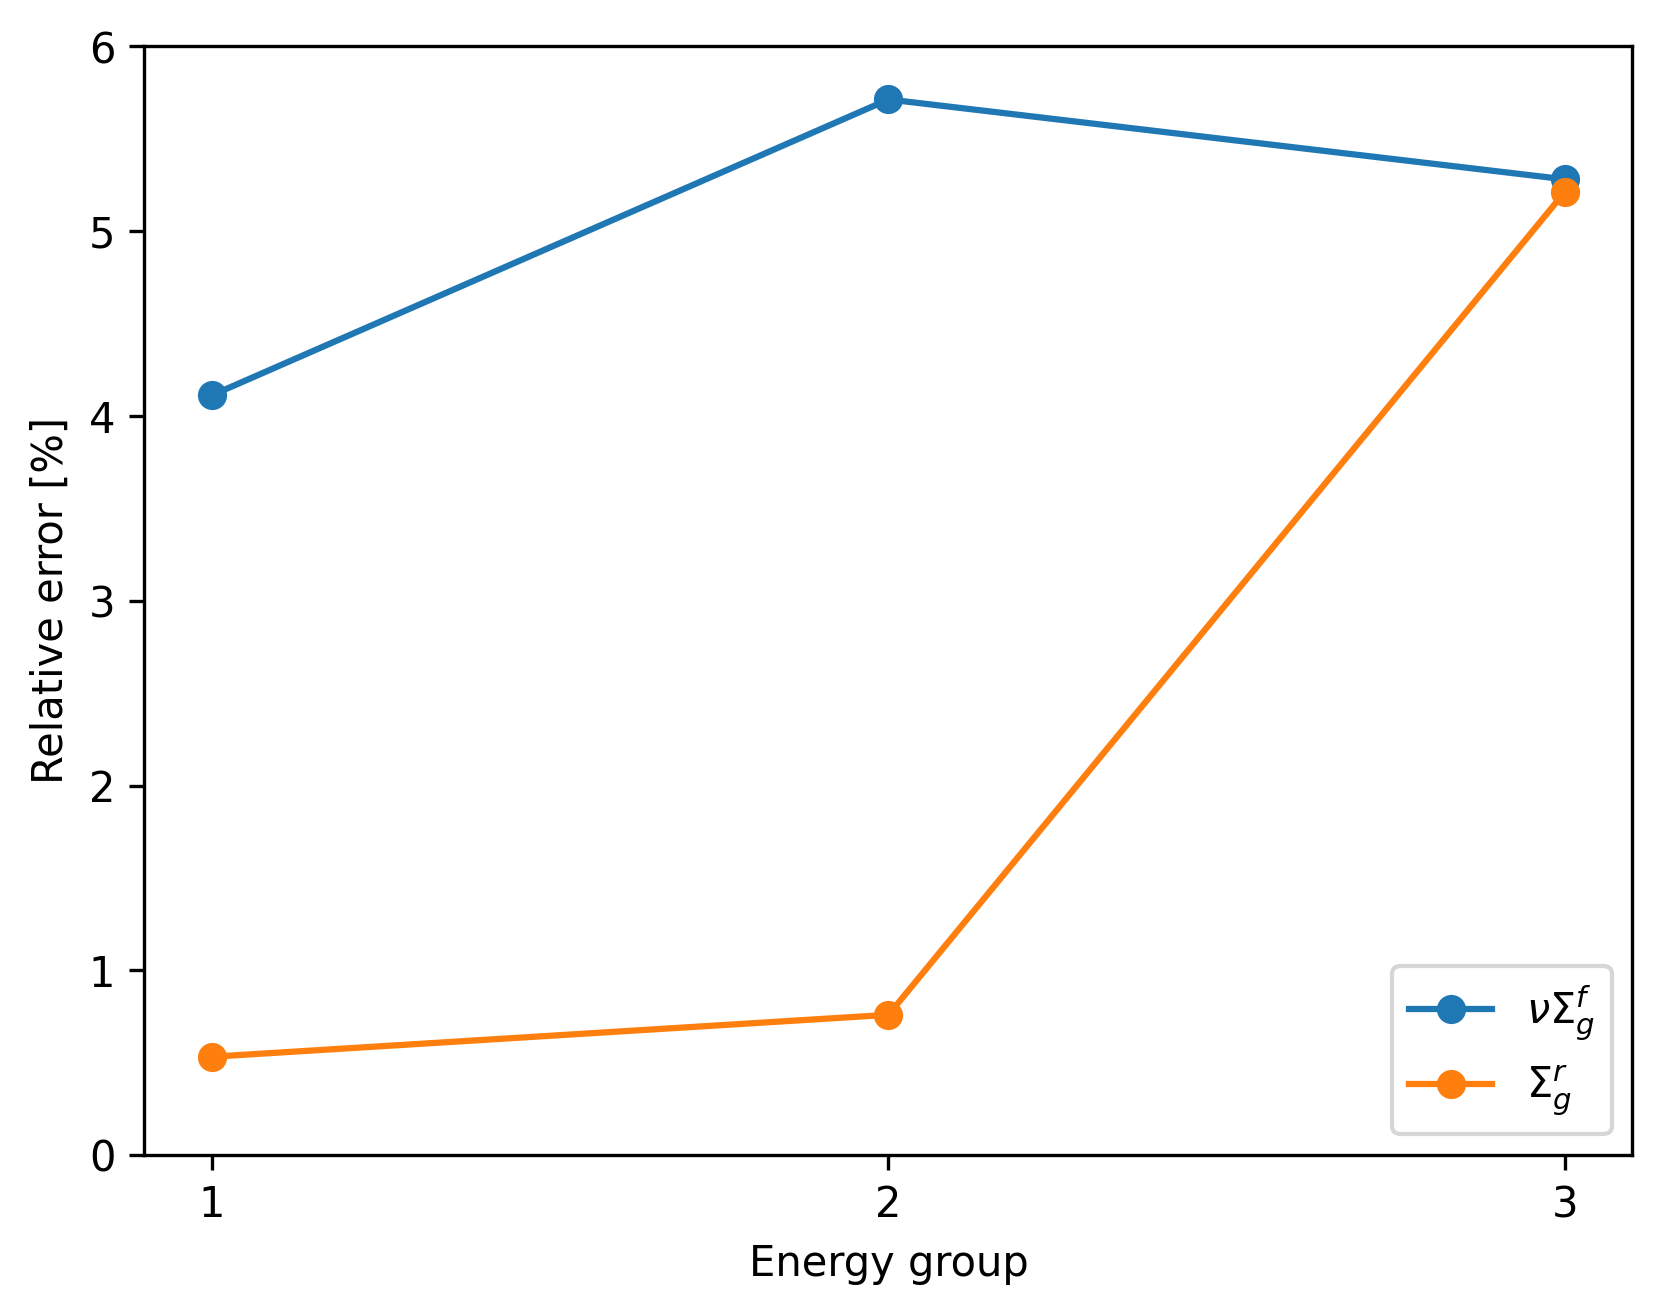
\includegraphics[width=0.43\linewidth]{figures/param-comparison}
	\hfill
	\caption{Relative error of the group constants generated with a homogeneous isotope distribution.}
	\label{fig:param-comparison}
\end{figure}

The results show that the homogenization of the fuel compact isotopes decreases the multiplication factor considerably.
The impact on the group constants does not seem to be substantial.
However, the multiplication factor's considerable difference suggests that the group constants’ small variations combined effect is significant.
Based on these results, Serpent models the TRISO particles explicitly in the following sections.


\subsection{Problem set-up}

% Diffusion calculations: homo vs hetero in LWRs
Diffusion calculations necessitate a spatial homogenization of the group constants.
Depending on the desired level of detail, the type of homogenization could vary.
For example, in PWR core calculations, the homogenization in space could be per assembly or pin-by-pin \cite{krebs_calculational_1990}.
In a per assembly homogenization, the diffusion code models a global neutronic representation of the assembly.
We will refer to diffusion calculations using this type of group constant homogenization scheme as homogeneous calculations.
A pin-by-pin homogenization makes possible the treatment of pin or assembly heterogeneities.
This type of homogenization yields a detailed neutronic representation of the fuel pins.
We will refer to diffusion calculations using this second type of homogenization scheme as heterogeneous calculations.

% Previous works using Moltres
Moltres is a heterogeneous solver.
Previous works \cite{lindsay_introduction_2018}\cite{pater_multiphysics_2019} have used Moltres for the analysis of \glspl{MSR}.
In such calculations, Moltres input files defined two materials: the moderator and the fuel.
For such a configuration, a node in the mesh representing the moderator holds the neutronics and temperature information only for the moderator.
The same is true in the fuel.
A homogeneous calculation would not differentiate between moderator and fuel and would hold the information of both materials in each node.

% What I did in this section:
Keeping in mind Moltres previous works, we aimed for a heterogeneous calculation in a prismatic \gls{HTGR}.
For such a calculation, we modeled a fuel column of the MHTGR-350 and generated the group constants using Serpent.
Figure \ref{fig:fuelcolumn} displays the Serpent model geometry.
We obtained the group constants for three materials: moderator, coolant, and fuel compact.
Serpent ran 5$\times 10^5$ neutrons/cycle, 400 active cycles, and 100 inactive cycles for the calculations.
% The \gls{Keff} was 1.41933.
Taking advantage of the problem's symmetry, Moltres modeled only one-twelfth of the fuel column, Figure \ref{fig:fuelcolumn}.
We made the geometry and mesh using Gmsh \cite{geuzaine_gmsh_2020}.
The diffusion calculation had 183667 \glspl{DoF}/energy-group.
The Moltres input file set an eigenvalue convergence tolerance of 1$\times$10$^{-8}$.
Moltres calculation used a two energy group structure with a thermal cutoff at 0.625eV.
The eigenvalue calculation did not converge.
Although several factors could contribute to this behavior, we focused on the validity of the diffusion calculations in such a system.

% \begin{figure}[htbp!]
% 	\centering
% 	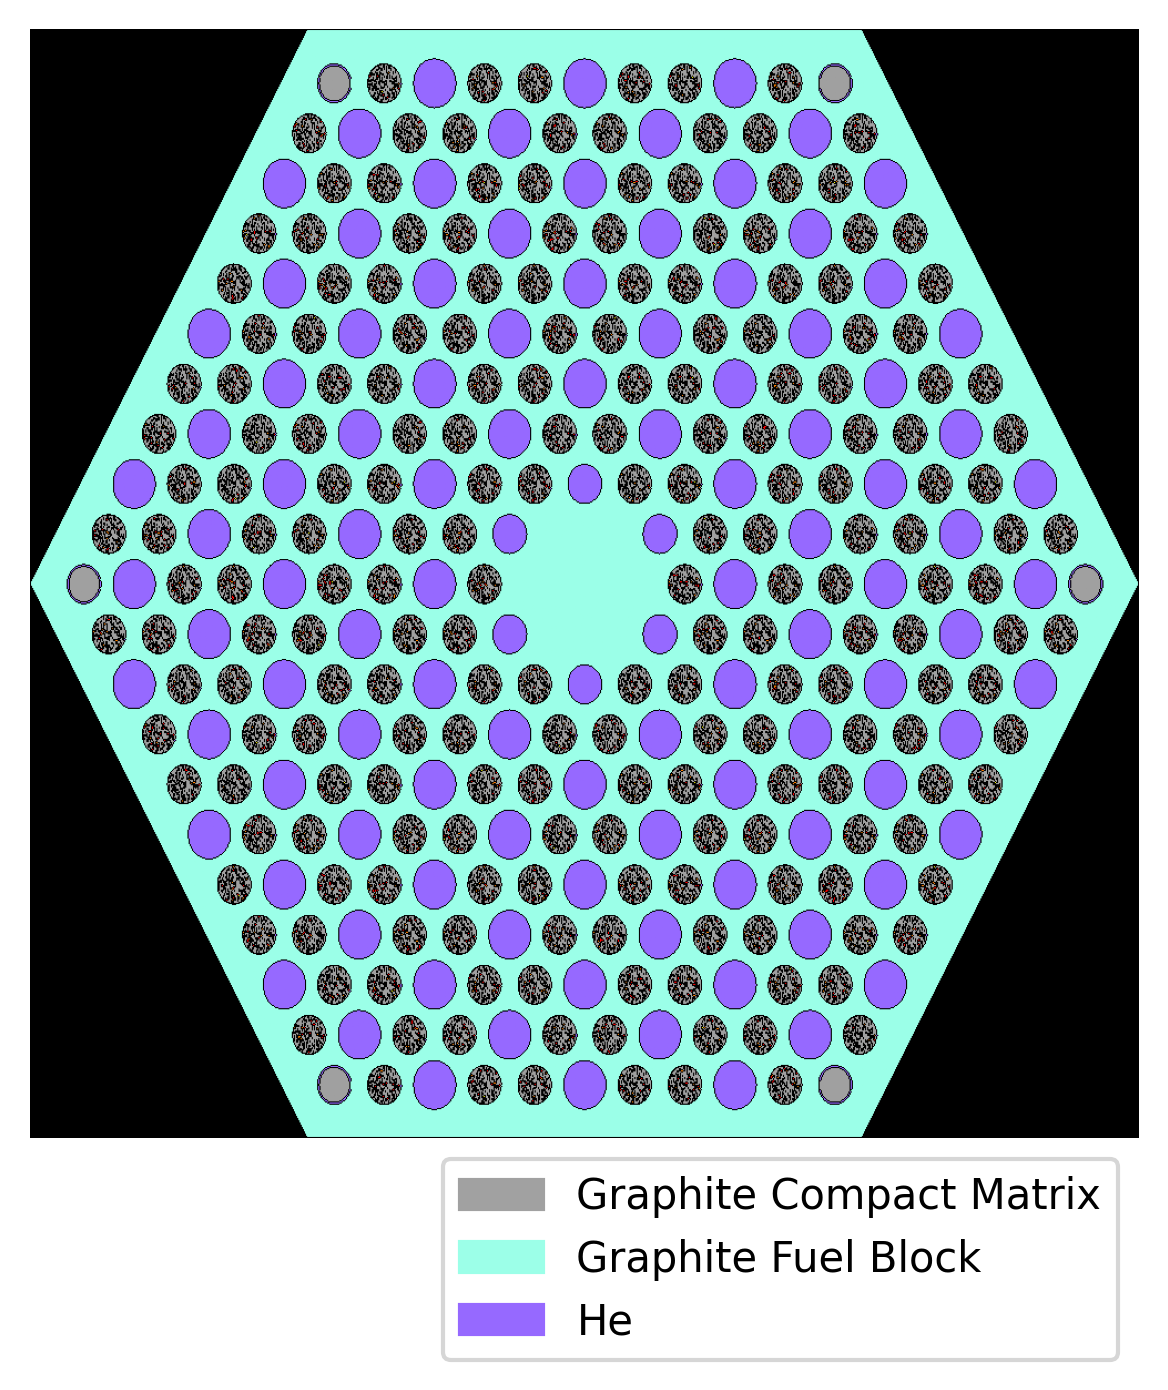
\includegraphics[width=0.45\linewidth]{figures-assembly/oecd-standard-column-legend}
% 	\hfill
% 	\caption{Serpent model of a MHTGR-350 fuel column.}
% 	\label{fig:fuelcolumn}
% \end{figure}

\begin{figure}[htbp!]
	\centering
    \subfloat[Serpent model geometry.]{
        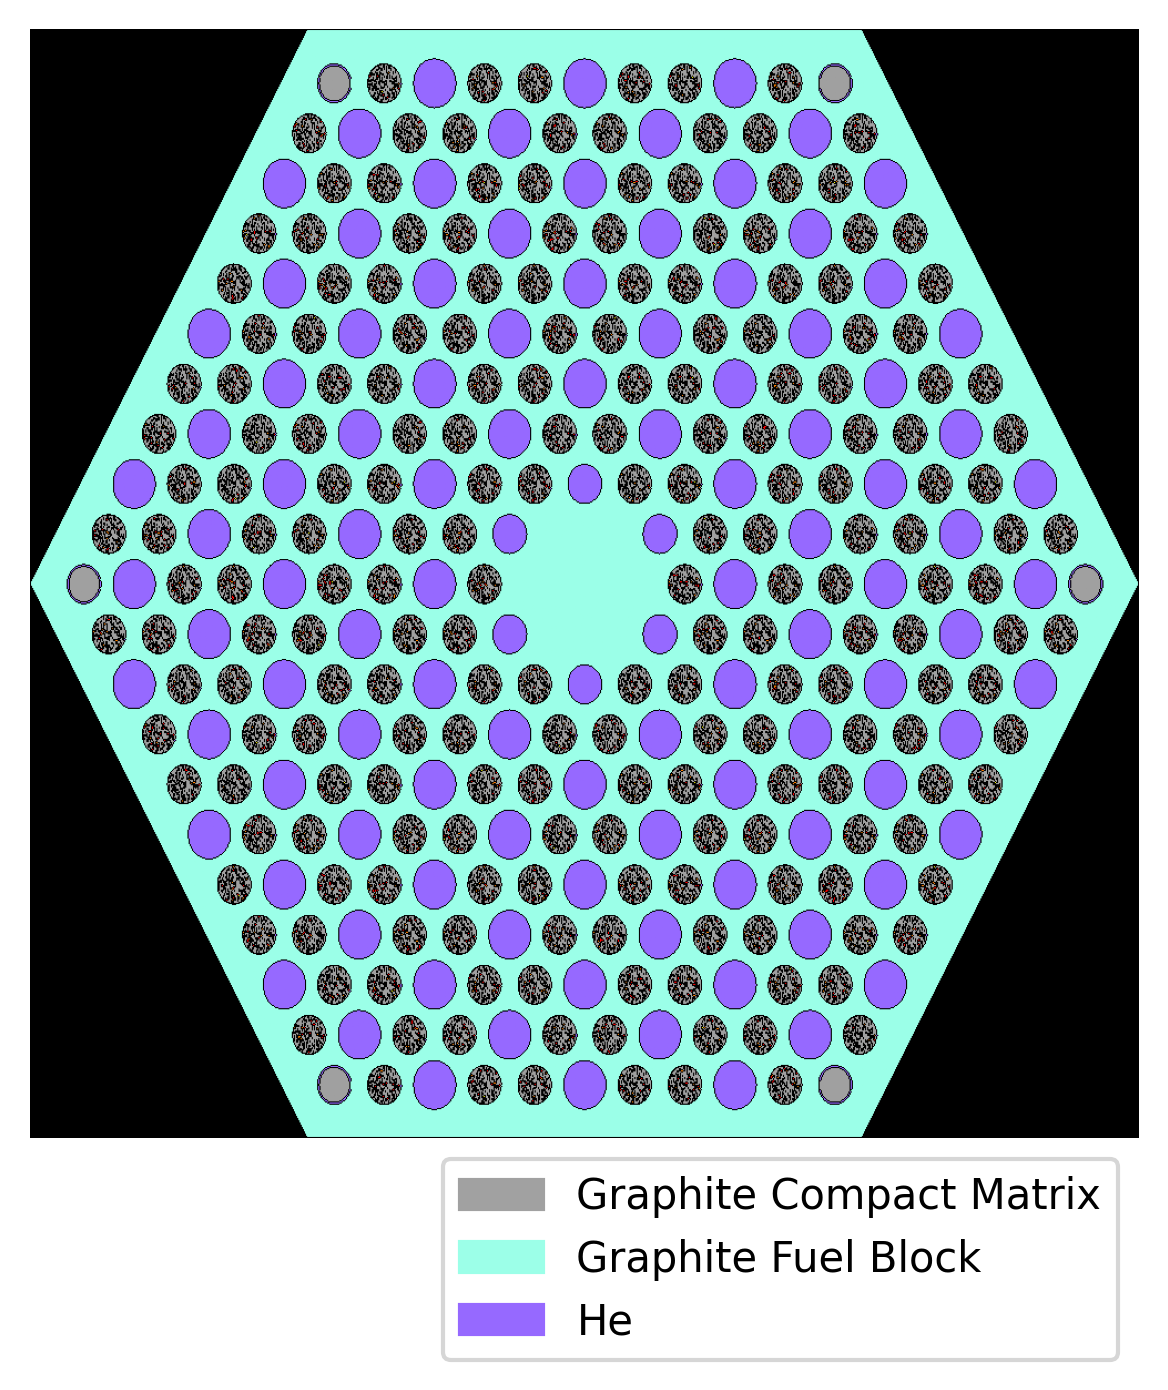
\includegraphics[width=0.35\textwidth]{figures-assembly/oecd-standard-column-legend}
    }
    \subfloat[Moltres model geometry.]{
        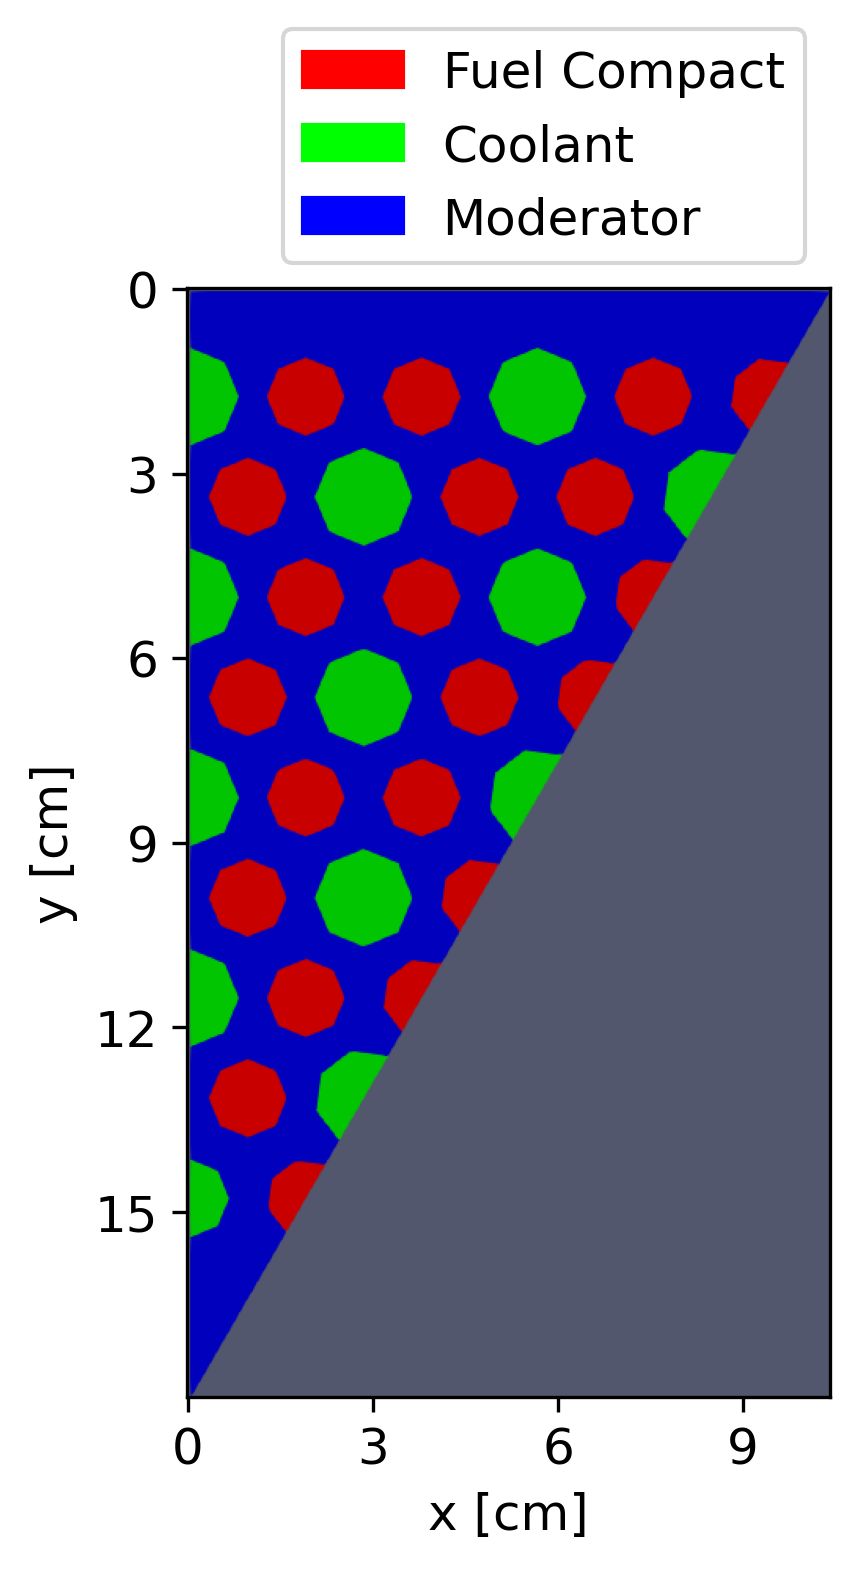
\includegraphics[width=0.22\textwidth]{figures-assembly/3D-assembly-30deg-reflec-meshB2}
    }
	\hfill
    \caption{Fuel column of the MHTGR-350. $xy$-plane in the active core region.}
	\label{fig:fuelcolumn}
\end{figure}

% Diffusion validity see bu1/tools-bu.txt
The diffusion theory considers that the current density is proportional to the gradient of the flux \cite{leppanen_development_2007}.
Such an approximation relies on the following assumptions:
\begin{itemize}
	\item The angular flux does not depend strongly on the angular variables.
	\item The fission source is isotropic.
	\item The time derivative of the current density is small compared to the mean collision time.
	\item The anisotropic energy-transfer is negligible in group-to-group scattering.
\end{itemize}

More detailed studies of the transport equation indicate that the following cases violate the assumption of a weak angular dependence \cite{duderstadt_nuclear_1976}:
\begin{itemize}
    \item Regions near vacuum boundaries and low-density material regions.
    \item Regions near strongly absorbing media.
    \item Regions near localized sources.
\end{itemize}

The diffusion theory applies best to geometries consisting of large homogeneous regions where the flux gradient is small.
This is the case for material regions whose geometrical scales are considerably larger than the neutron mean free path.
For this reason, we compared the neutron mean free path in the different fuel assembly materials, Table \ref{tab:mfp}.
The mean free path in the fuel compact and the moderator are in the order of the centimeters.
In the coolant, the mean free path magnitude is comparable to the fuel column dimensions.
These results suggest that a heterogeneous diffusion calculation of the prismatic fuel column violates the diffusion theory assumptions.

\begin{table}[htbp!]
  \centering
  \caption{Neutron mean free path in different materials. Values expressed in $cm$.}
  \begin{tabular}{l|cccc}
  \toprule
              & Fuel compact  & Moderator  & Coolant  & Homogeneous fuel \\
  \midrule
  Fast  		& 2.71 & 2.70 & 1137.31 & 3.37 \\
  Thermal		& 2.22 & 2.36 & 1945.49 & 2.89 \\

  \bottomrule
  \end{tabular}
  \label{tab:mfp}
\end{table}

As the next step, we conducted a feasibility study for the homogeneous calculation of the fuel assembly in Moltres.
Serpent calculated the homogeneous group constants of the fuel assembly.
We homogenized the fuel, coolant, and moderator to create a 'homogeneous fuel.'
This material's mean free path is in the order of the centimeters, Table \ref{tab:mfp}.
Next, Moltres used the homogeneous group constants to carry out an eigenvalue calculation.
We compared Moltres results with Serpent results.
Serpent's \gls{Keff} was 1.41933 while Moltres' was 1.4078788.
Moltres eigenvalue is smaller than Serpent's eigenvalue.
Additionally, we obtained the axial flux in the fuel column.
Figure \ref{fig:prelim} displays a comparison between Serpent and Moltres axial fluxes.
Serpent's flux is the average flux over the fuel column volume.
Moltres flux is the point-wise flux over the $z$-axis.
The fluxes are similar in shape and magnitude.

% Conclusion
We empathize that this was a feasibility study.
The following sections make a more in-depth analysis of more detailed results.
Based on these results and discussion, we use Moltres for carrying out homogeneous calculations in the following sections.

\begin{figure}[htbp!]
	\centering
    \subfloat[Serpent.]{
        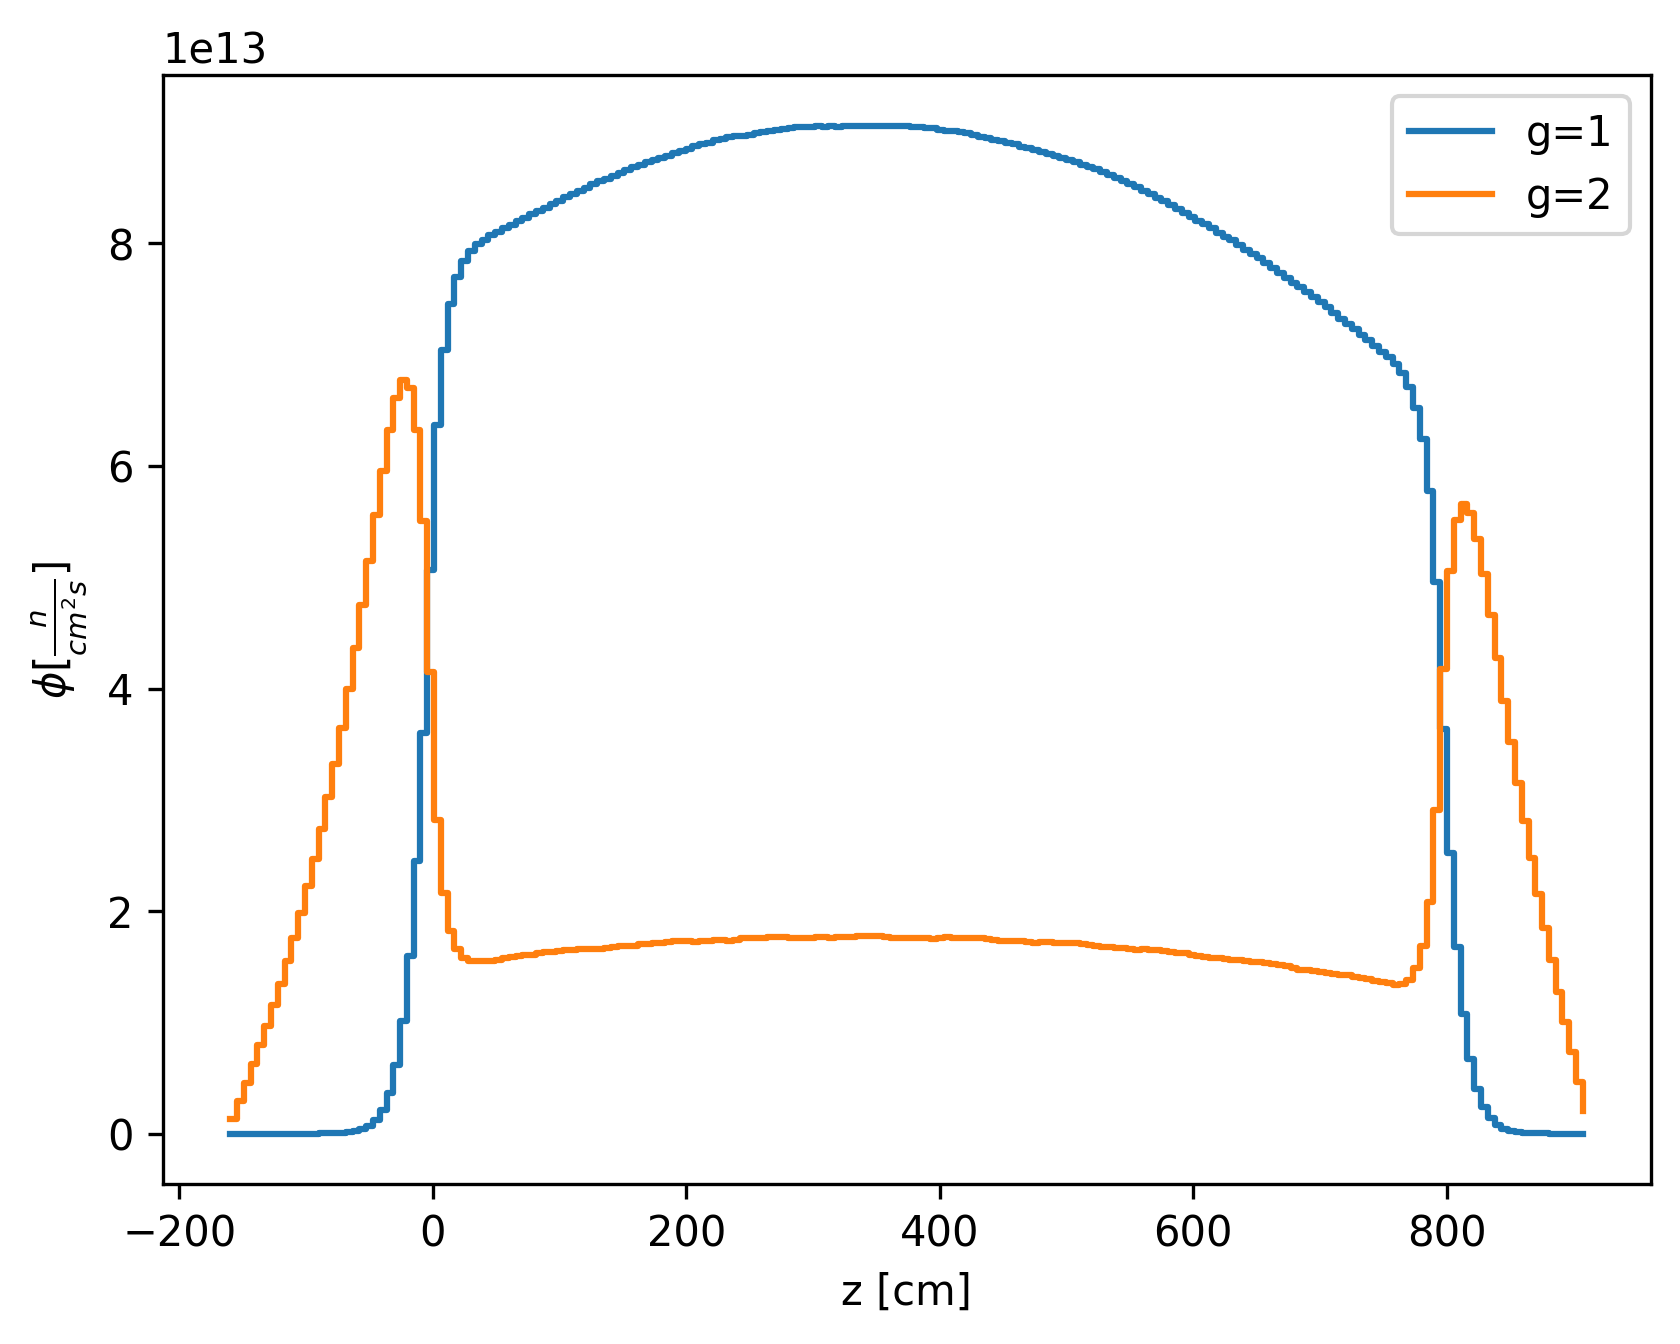
\includegraphics[width=0.45\textwidth]{figures/standard-column-detector-Axial}
    }
    \subfloat[Moltres.]{
        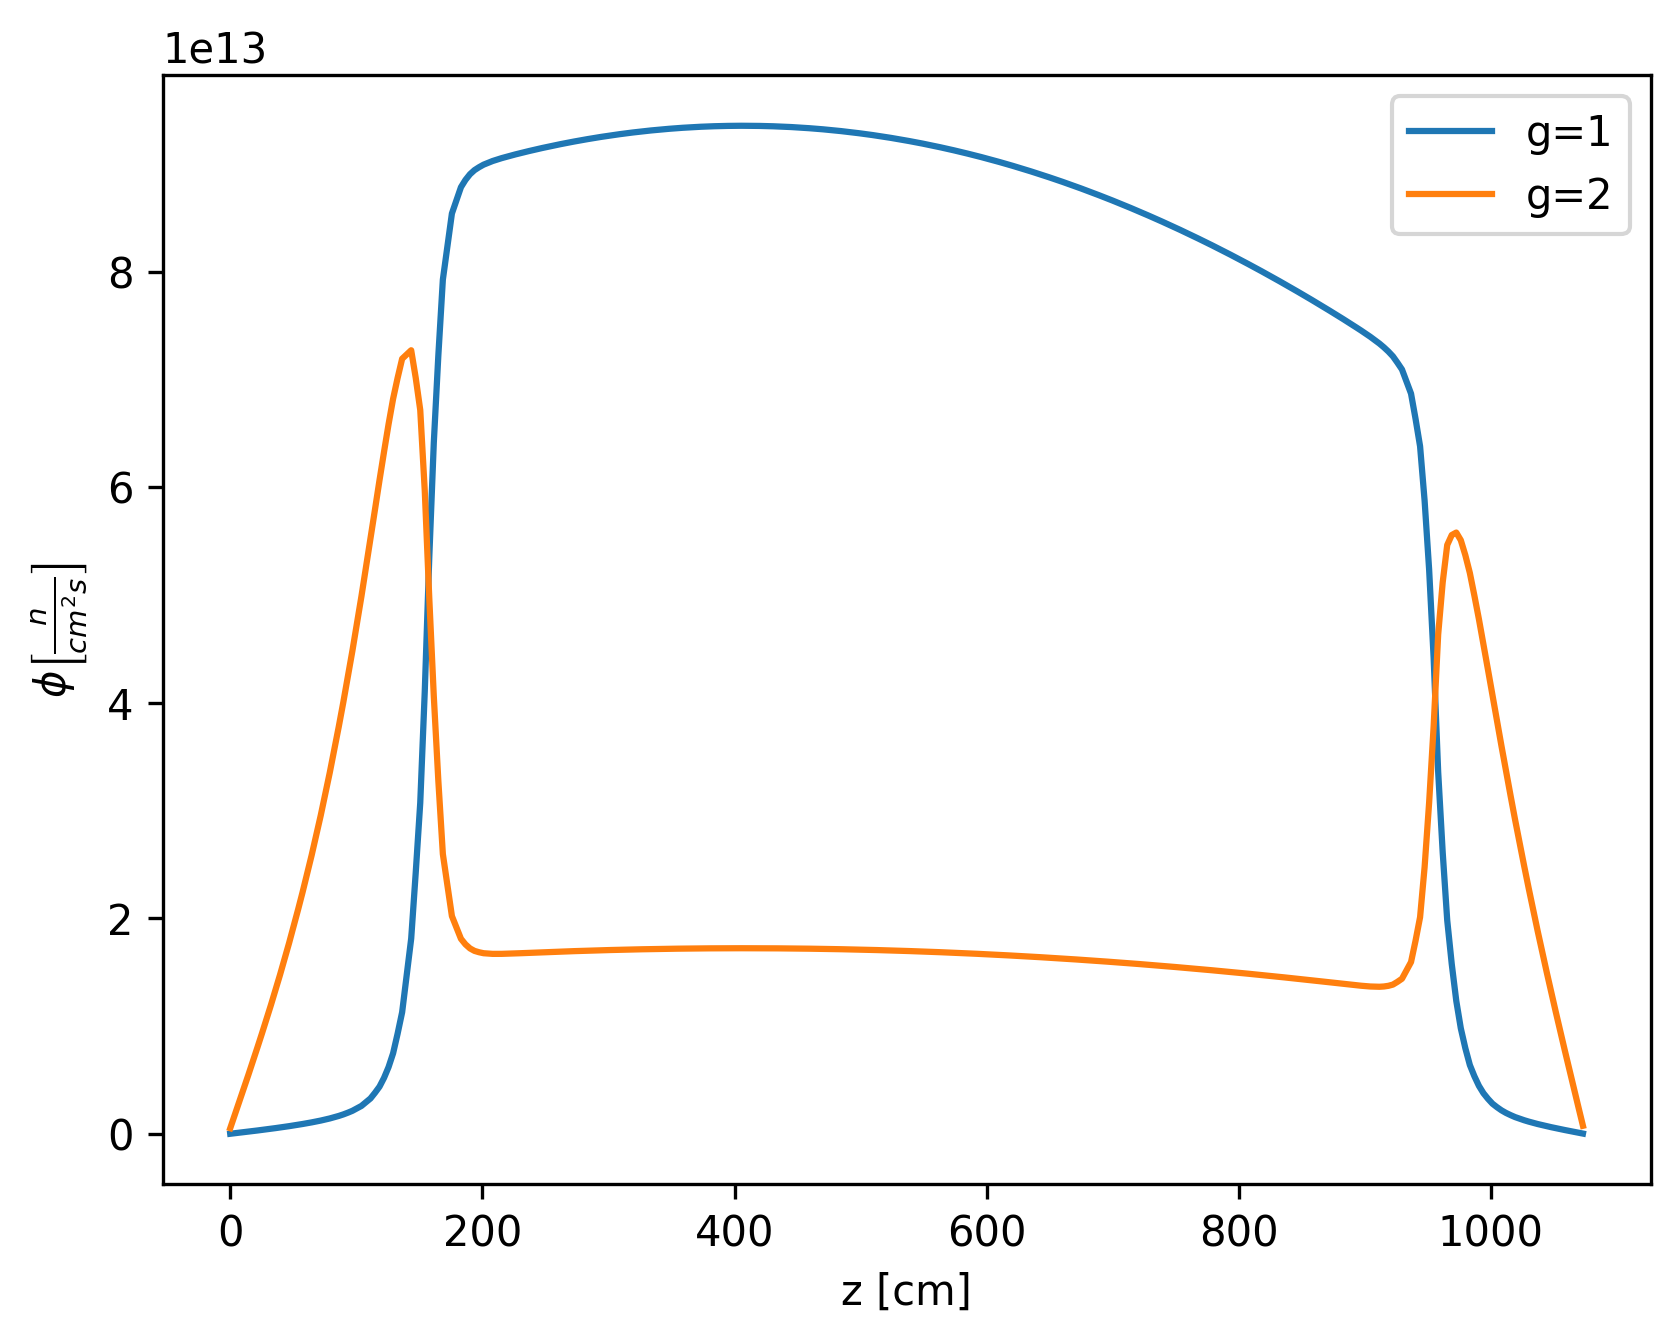
\includegraphics[width=0.45\textwidth]{figures/homo-fuel}
    }
	\hfill
  \caption{Two group axial flux comparison.}
	\label{fig:prelim}
\end{figure}

\section{Serpent-Moltres comparison}

\subsection{Fuel column}

\begin{table}[htbp!]
  \centering
  \caption{Energy group structure.}
  \begin{tabular}{c|l|l|l|l|l|l|l|l|l|l|l|l}
  \toprule
  Upper boundary [eV] & 26    & 21   & 18   & 15a & 15b & 15c & 15d & 15e   & 12  & 9  & 6  & 3 \\
  \midrule
  1.49E+07            & 1     & 1    & 1    & 1   & 1   & 1   & 1   & 1     & 1   & 1  & 1  & 1 \\ \cline{1-2}
  7.41E+06            & 2     &      &      &     &     &     &     &       &     &    &    &   \\ \cline{1-10}
  3.68E+06            & 3     & 2    & 2    & 2   & 2   & 2   & 2   & 2     & 2   &    &    &   \\ \cline{1-2}
  6.72E+05            & 4     &      &      &     &     &     &     &       &     &    &    &   \\ \hline
  1.11E+05            & 5     & 3    & 3    & 3   & 3   & 3   & 3   & 3     & 3   & 2  & 2  & 2 \\ \cline{1-6} \cline{10-10}
  1.93E+04            & 6     & 4    & 4    & 4   & 4   &     &     &       & 4   &    &    &   \\ \cline{1-2}
  3.35E+03            & 7     &      &      &     &     &     &     &       &     &    &    &   \\ \cline{1-4} \cline{7-7}
  1.58E+03            & 8     & 5    & 5    &     &     & 4   &     &       &     &    &    &   \\ \cline{1-6} \cline{8-11}
  7.48E+02            & 9     & 6    & 6    & 5   & 5   &     & 4   & 4     & 5   & 3  &    &   \\ \cline{1-7} \cline{10-11}
  2.75E+02            & 10    & 7    & 7    & 6   & 6   & 5   &     &       & 6   & 4  &    &   \\ \cline{1-6} \cline{8-12}
  1.30E+02            & 11    & 8    & 8    & 7   & 7   &     & 5   & 5     & 7   & 5  & 3  &   \\ \cline{1-3} \cline{6-7}
  6.14E+01            & 12    & 9    &      &     & 8   & 6   &     &       &     &    &    &   \\ \cline{1-6} \cline{8-9}
  2.90E+01            & 13    & 10   & 9    & 8   & 9   &     & 6   & 6     &     &    &    &   \\ \cline{1-5} \cline{10-11}
  1.37E+01            & 14    & 11   & 10   & 9   &     &     &     &       & 8   & 6  &    &   \\ \cline{1-10}
  8.32E+00            & 15    & 12   & 11   & 10  & 10  & 7   & 7   & 7     & 9   &    &    &   \\ \cline{1-2}
  5.04E+00            & 16    &      &      &     &     &     &     &       &     &    &    &   \\ \hline
  2.38E+00            & 17    & 13   & 12   & 11  & 11  & 8   & 8   & 8     & 10  & 7  & 4  & 3 \\ \cline{1-3}
  1.29E+00            & 18    & 14   &      &     &     &     &     &       &     &    &    &   \\ \cline{1-12} 
  6.50E-01            & 19    & 15   & 13   & 12  & 12  & 9   & 9   & 9     & 11  & 8  & 5  &   \\ \cline{1-3} \cline{7-8}
  3.50E-01            & 20    & 16   &      &     &     & 10  & 10  &       &     &    &    &   \\ \cline{1-9}
  2.00E-01            & 21    & 17   & 14   & 13  & 13  & 11  & 11  & 10    &     &    &    &   \\ \cline{1-2} \cline{9-9}
  1.20E-01            & 22    &      &      &     &     &     &     & 11    &     &    &    &   \\ \cline{1-9} 
  8.00E-02            & 23    & 18   & 15   & 14  & 14  & 12  & 12  & 12    &     &    &    &   \\ \cline{1-4} \cline{7-9}
  5.00E-02            & 24    & 19   & 16   &     &     & 13  & 13  & 13    &     &    &    &   \\ \hline
  2.00E-02            & 25    & 20   & 17   & 15  & 15  & 14  & 14  & 14    & 12  & 9  & 6  &   \\ \cline{1-4} \cline{7-9}
  1.00E-02            & 26    & 21   & 18   &     &     & 15  & 15  & 15    &     &    &    &   \\
  \bottomrule
  \end{tabular}
  \label{tab:energygroups}
\end{table}

In this section, we investigated the effects of the energy group structure on the diffusion simulations.
We conducted two analyses.
First, we varied the number of energy groups.
Second, we tried different energy group structures for the same number of groups.
To reduce the computational expense, we narrowed down our focus to a fuel column of the MHTGR-350, Figure \ref{fig:fuelcolumn}.
The fuel column includes the bottom and top reflectors.
Tables \ref{tab:element-characteristics} and \ref{tab:compact} specify the model input parameters.

The first step in the calculation was to obtain the group constants using Serpent.
Figure \ref{fig:fuelcolumn} displays a $xy$-plane of the model.
To simplify Serpent's model, we did not consider the fuel handling holes or the bottom and top reflectors' coolant channels.
\glspl{HTGR} use \glspl{LBP} to reduce the power peaking factors in different active core regions.
Some reactors could have \glspl{LBP} in the rings closer to the reflectors, and no \glspl{LBP} in the middle rings.
This characteristic motivated the analysis of two cases, a fuel column that does not have \glspl{LBP}, and one that has.
The LBP's locations are the six corners of the fuel assembly, Figure \ref{fig:fuelassembly}.
The material temperatures were 600K and 1200K, cases that represent the \gls{CZP} and the \gls{HFP} core states.
Serpent ran 4$\times 10^5$ neutrons/cycle, 360 active cycles, and 40 inactive cycles for the calculations.

Taking advantage of the problem's symmetry, Moltres modeled only one-twelfth of the fuel column.
We made the geometry and mesh using Gmsh.
The mesh had 37120 elements and 22862 nodes.
The diffusion calculations had 22862 \glspl{DoF}/energy-group.
The Moltres input files set an eigenvalue and a flux convergence tolerance of 1$\times$10$^{-8}$.
Moltres calculations used different energy group structures listed in Table \ref{tab:energygroups}.

% This is very important and I should review it carefully
To compare the results from Serpent and Moltres, we present figure comparing the three-group axial fluxes.
Moltres ran the calculations for 26 energy groups and collapsed the results into three energy groups to facilitate the results' visualization.
Note that Serpent's flux is an average over the volume, while the Moltres' flux is the point-wise flux over a line.
Another figure compares the eigenvalue from Serpent and eigenvalues from Moltres for the different energy group structures.
The last analysis is for the Moltres axial flux.
Considering the 26 group structure as the reference value, we obtained the $L_2$-norm of the active core's axial flux relative error.

% Fluxes
To recapitulate, we simulated four operational cases: no \gls{LBP} at 600K, no \gls{LBP} at 1200K, \gls{LBP} at 600K, and \gls{LBP} at 1200K.
Figures \ref{fig:assembly-noLBP-600-flux} to \ref{fig:assembly-LBP-1200-flux} display the axial flux from the Serpent and the Moltres simulations for all cases.
For the no LBP at 600K case, the fluxes are close in shape and magnitude.
For the no LBP at 1200K case, the fluxes look similar.
The flux in Moltres has a straighter shape.
The thermal flux peak in the bottom reflector is bigger.
For the LBP at 600K case, the flux in Moltres has a larger magnitude.
Additionally, the shape of the Moltres flux is concave, while the Serpent flux is convex.
For the LBP at 1200K case, the flux in Moltres is larger.
The Moltres flux is more concave than the Serpent flux.
Overall, the fluxes in Moltres and Serpent are close in shape and magnitude.

% No LBP 600
\begin{figure}[htbp!]
	\centering
    \subfloat[Moltres.]{
        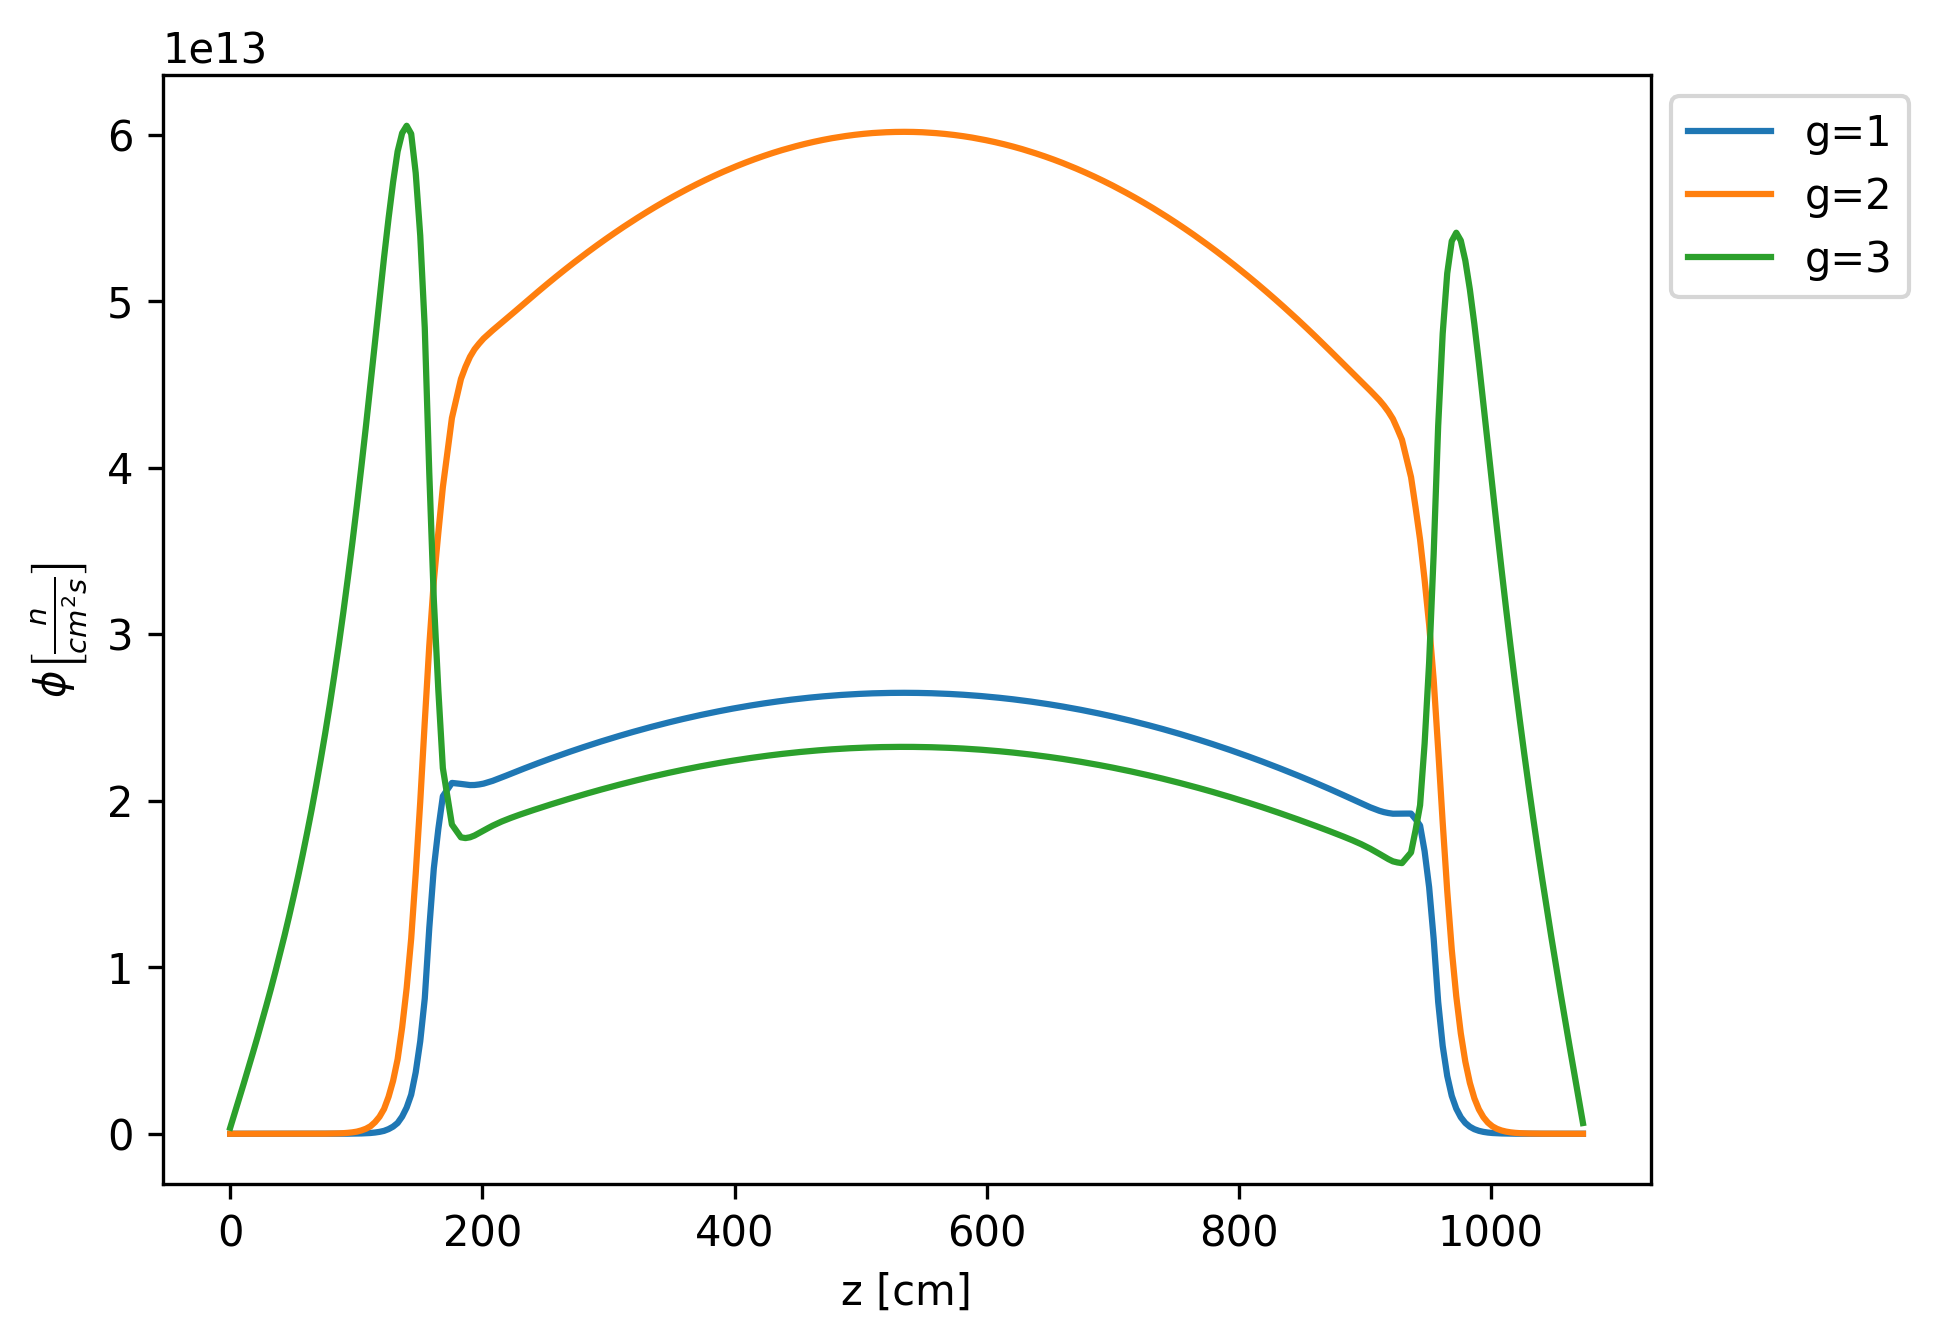
\includegraphics[width=0.45\textwidth]{figures-assembly/3D-assembly-noLBP-600-26G}
    }
    \subfloat[Serpent.]{
        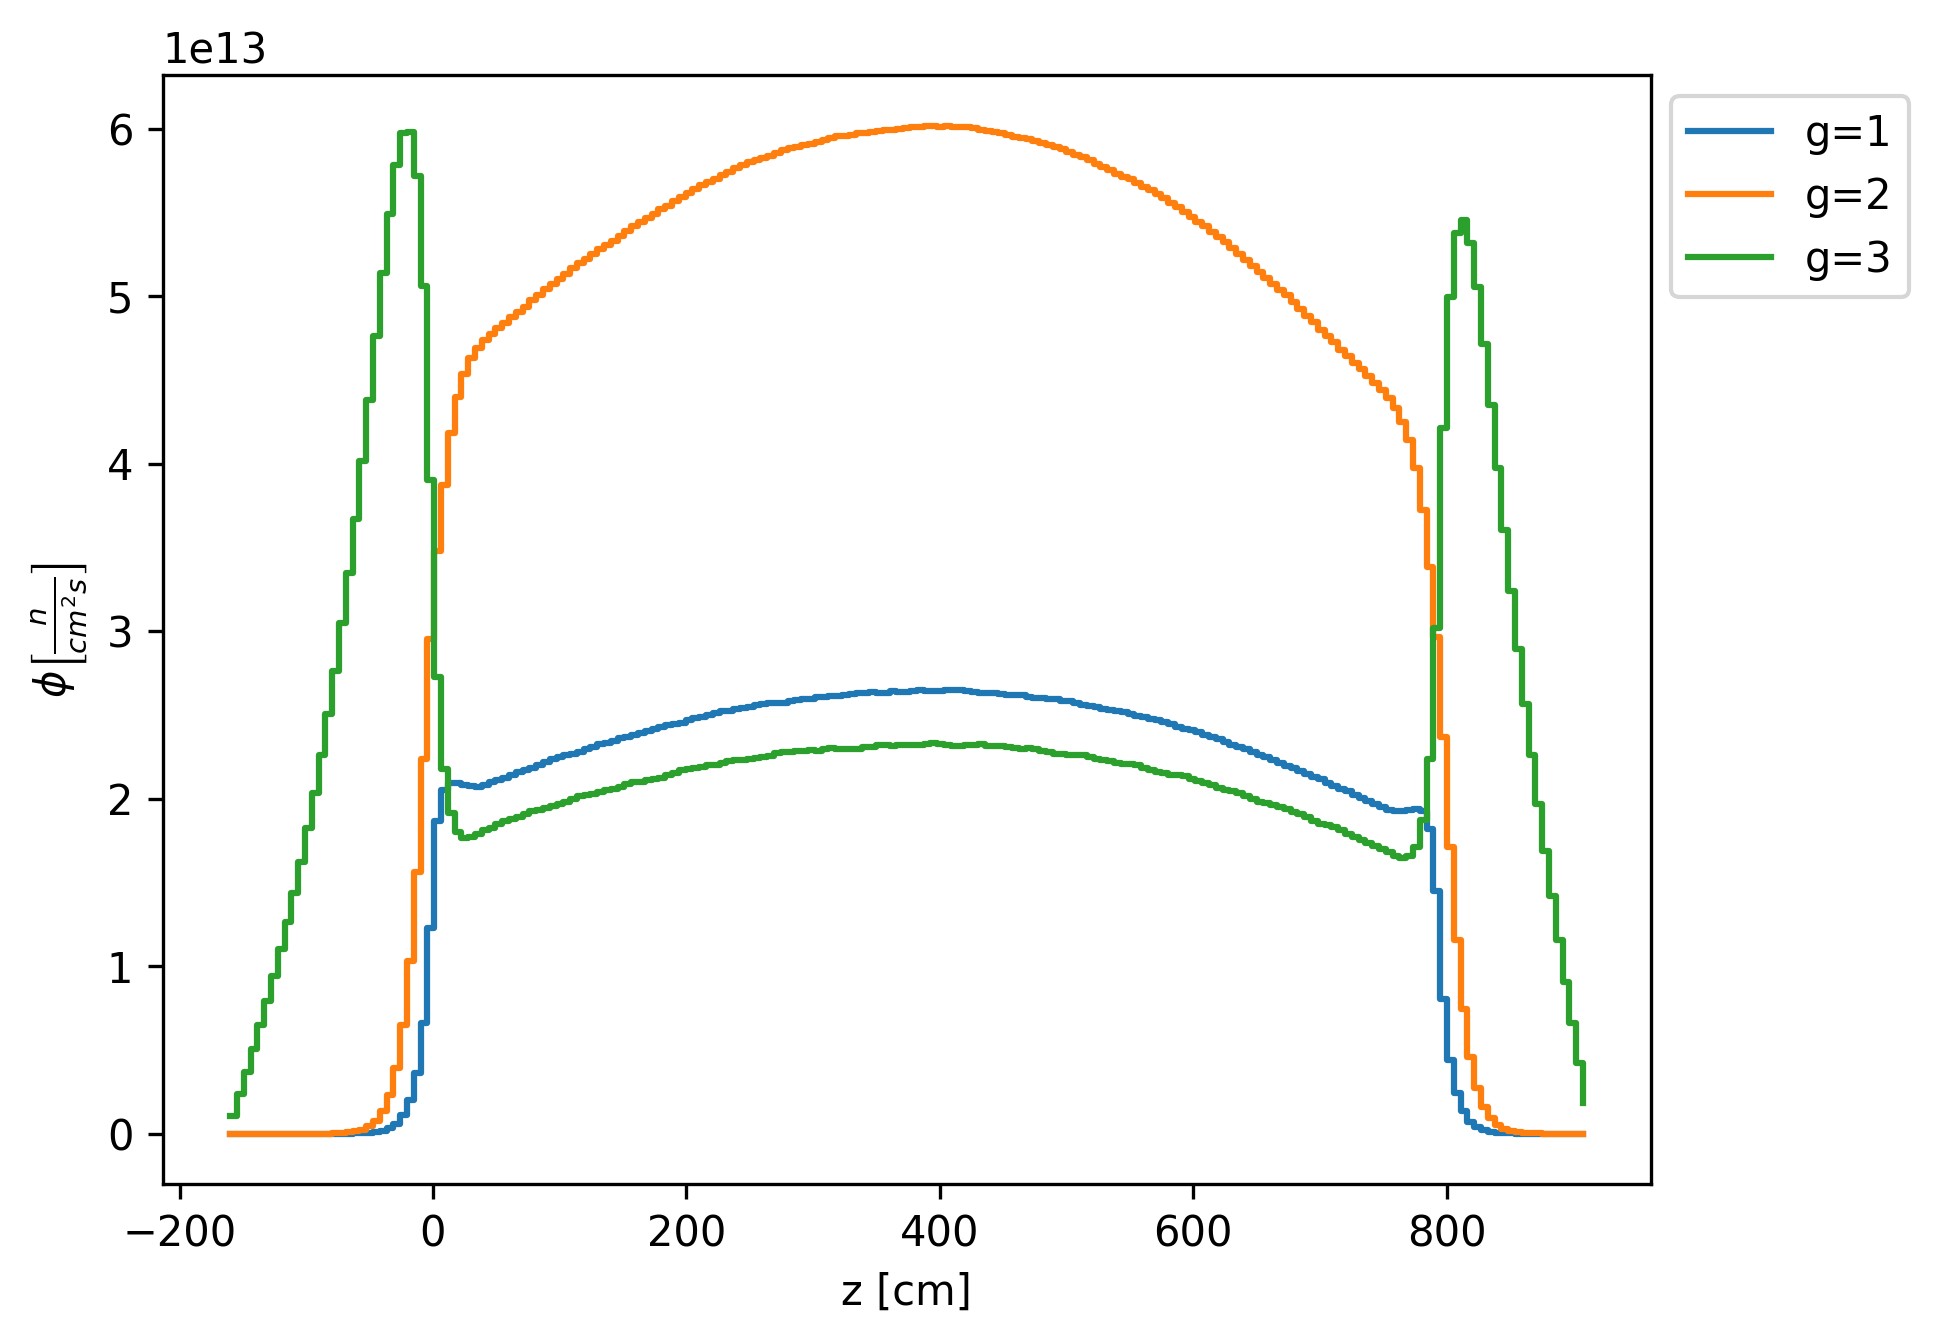
\includegraphics[width=0.45\textwidth]{figures-assembly/serpent26G-noLBP-600-collapse}
    }
	\hfill
    \caption{Case no LBP at 600K. 3-group axial neutron flux.}
	\label{fig:assembly-noLBP-600-flux}
\end{figure}

% No LBP 1200
\begin{figure}[htbp!]
  \centering
    \subfloat[Moltres.]{
        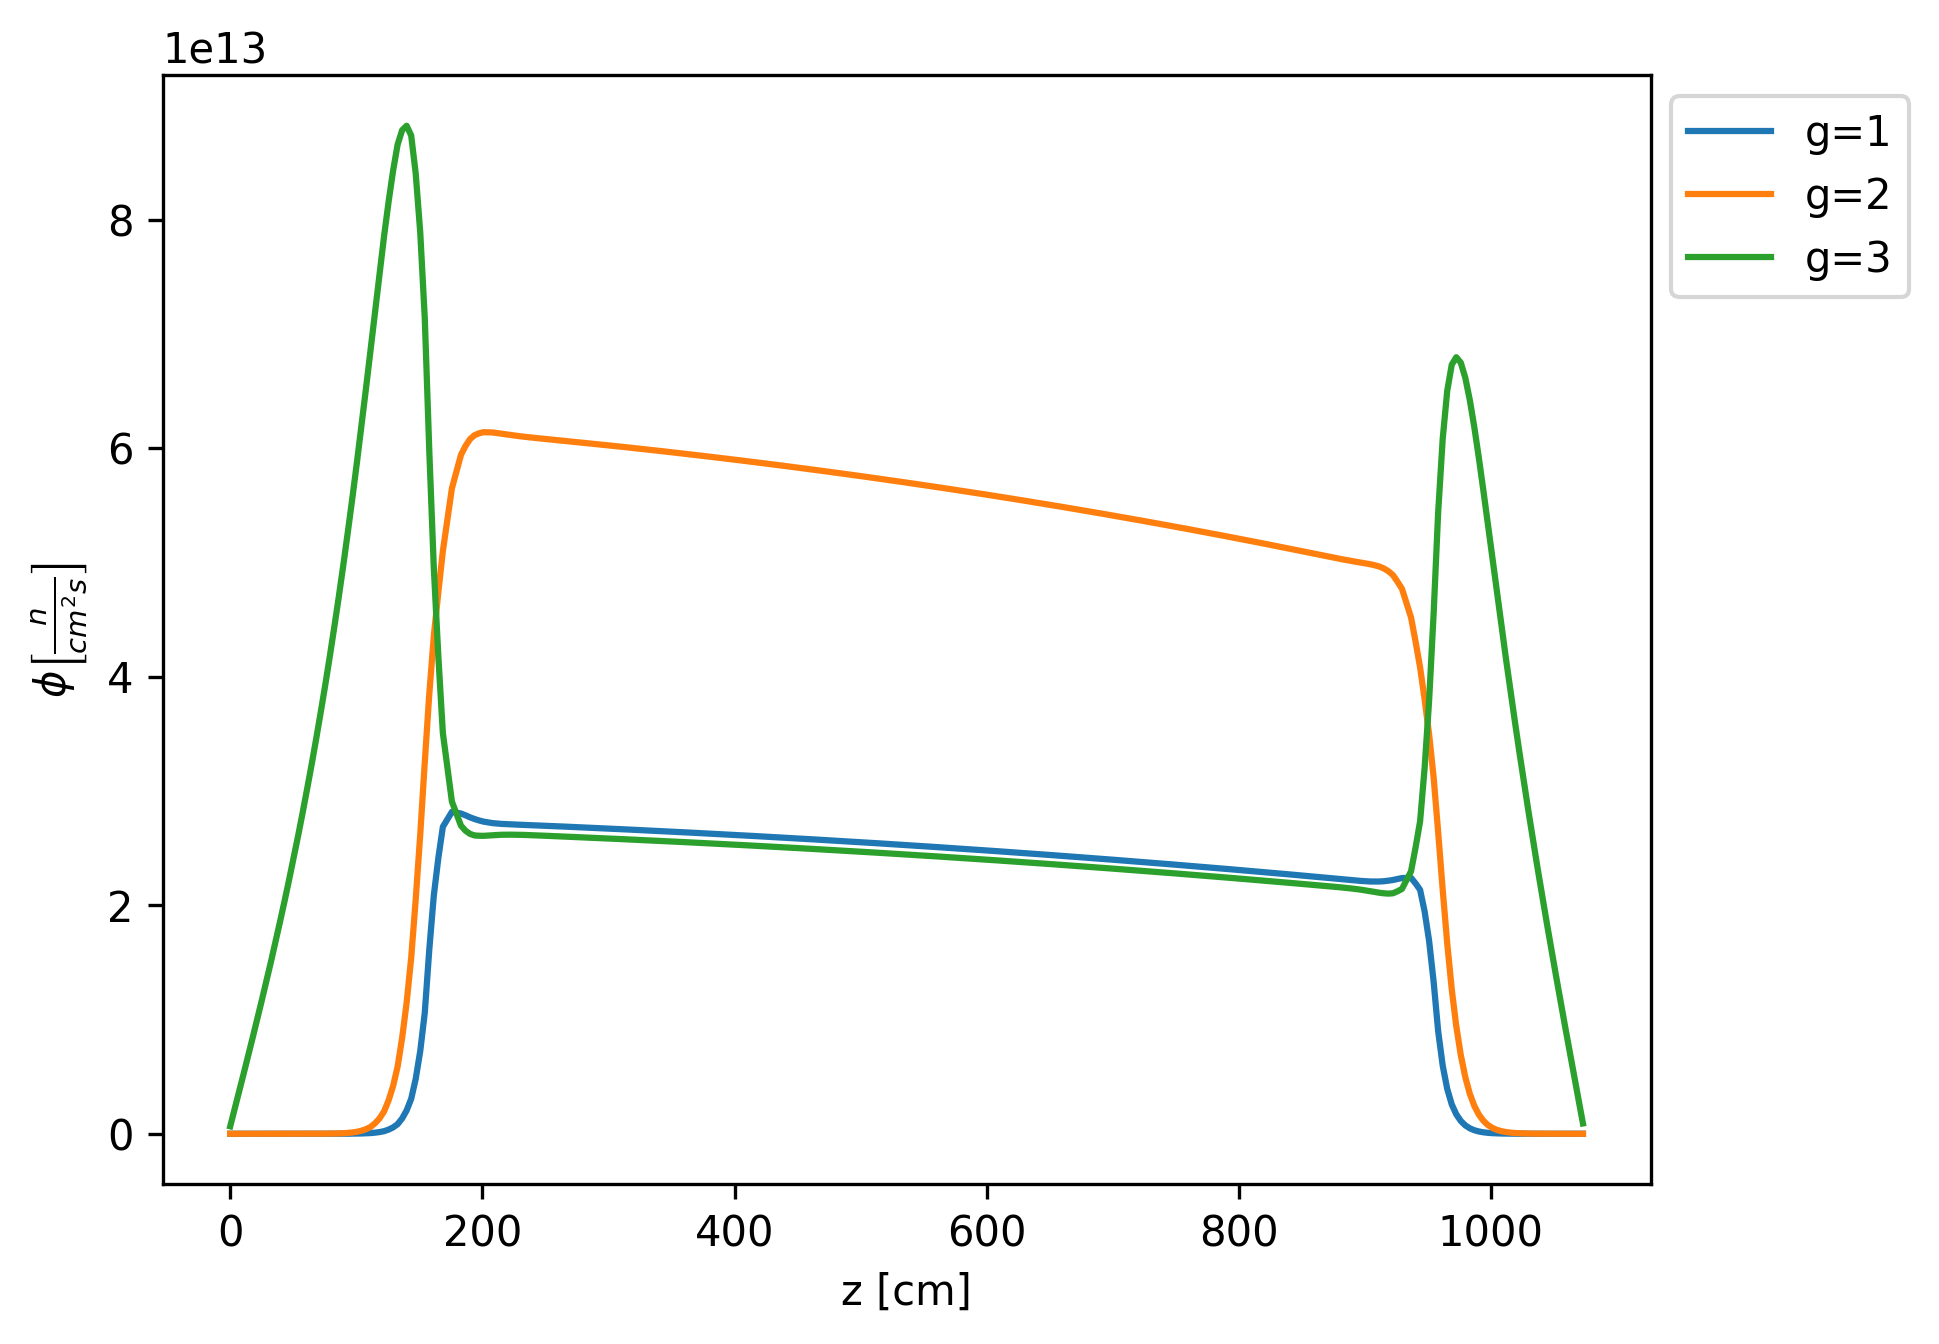
\includegraphics[width=0.45\textwidth]{figures-assembly/3D-assembly-noLBP-1200-26G}
    }
    \subfloat[Serpent.]{
        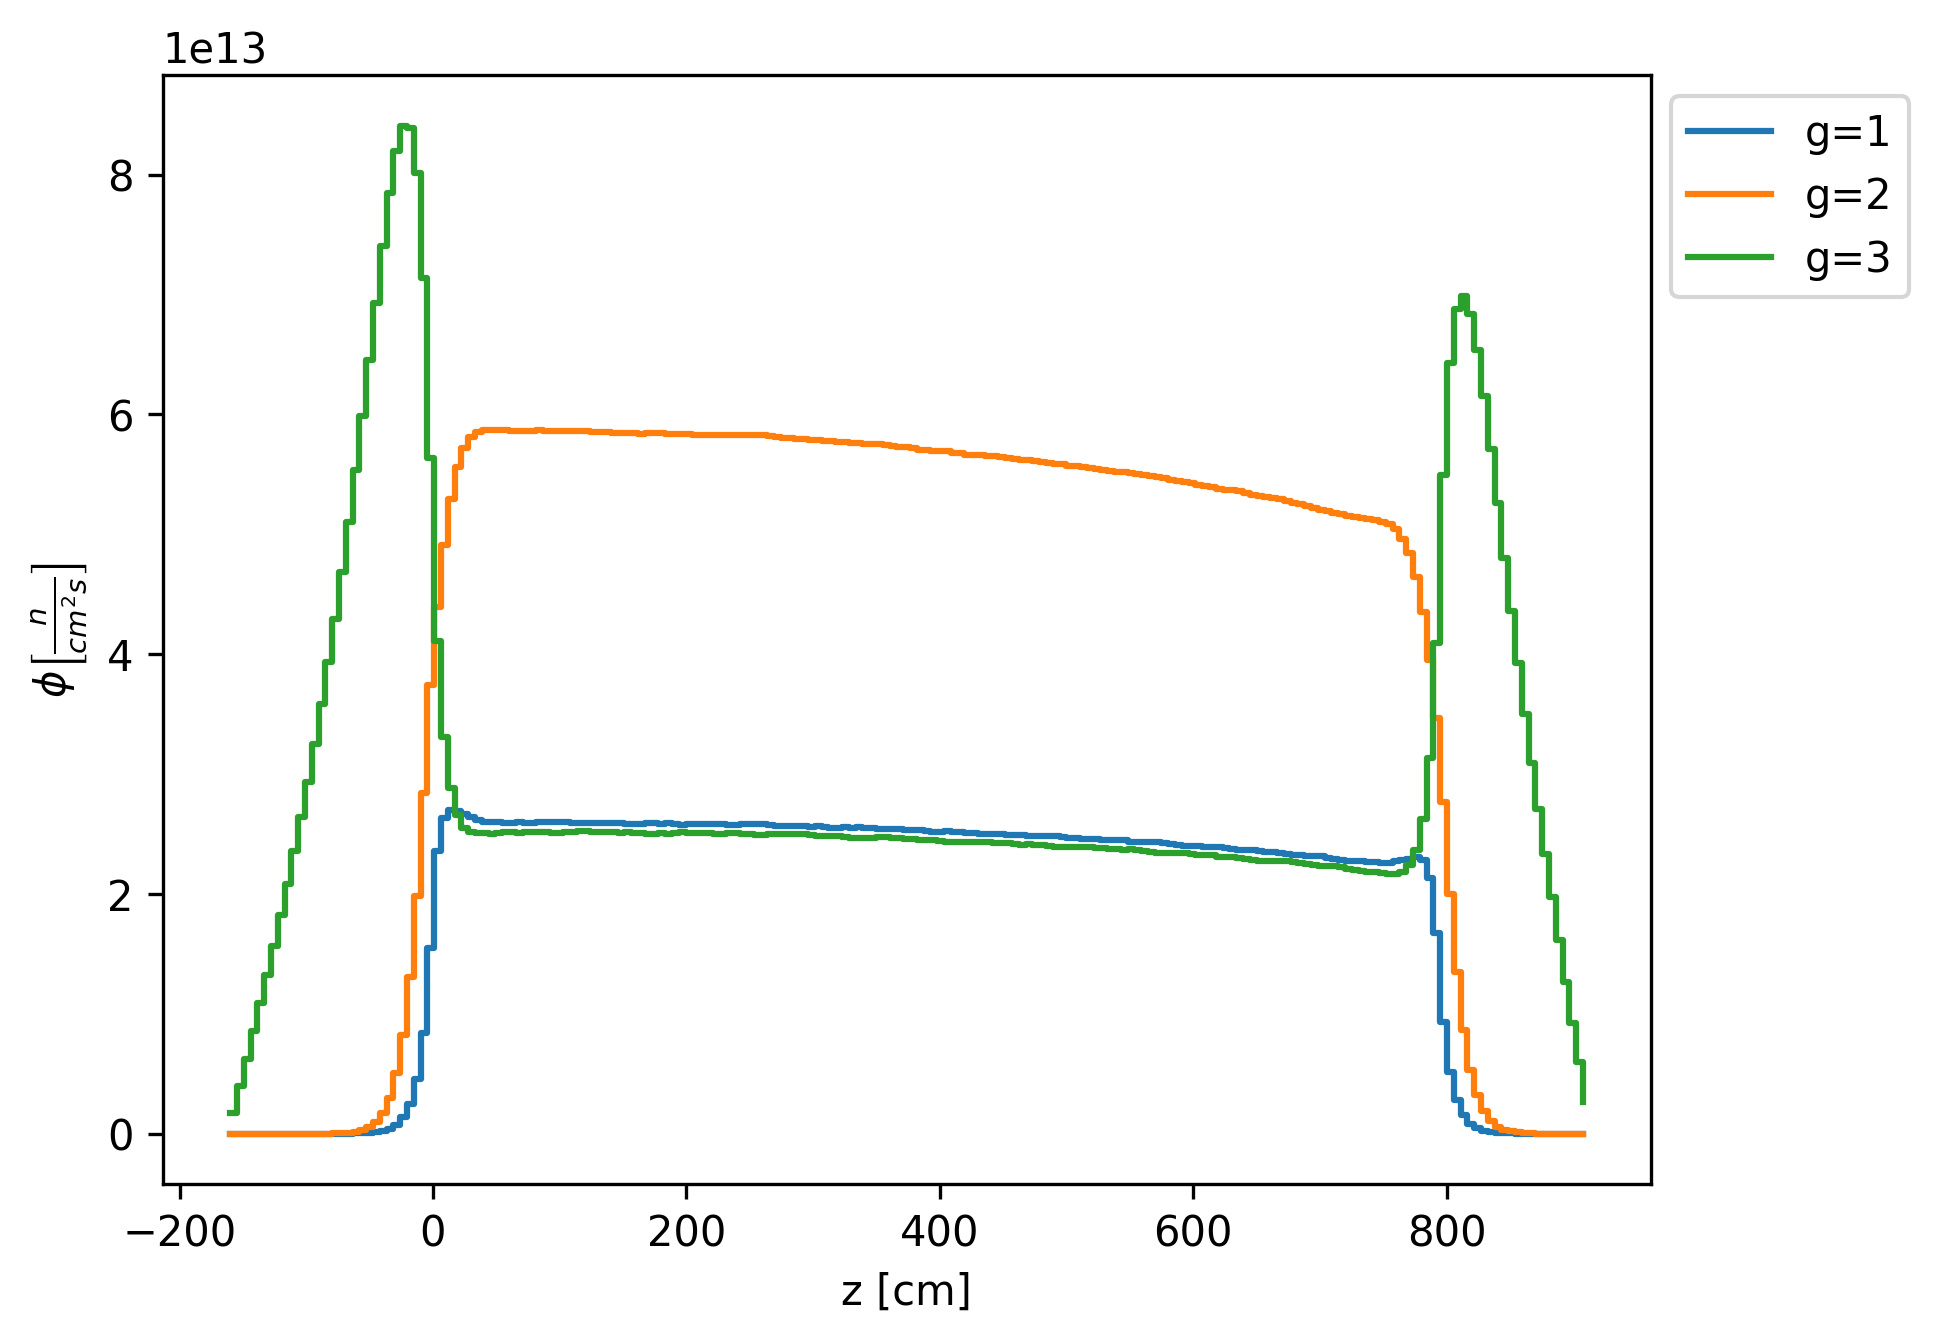
\includegraphics[width=0.45\textwidth]{figures-assembly/serpent26G-noLBP-1200-collapse}
    }
  \hfill
    \caption{Case no LBP at 1200K. 3-group axial neutron flux.}
  \label{fig:assembly-noLBP-1200-flux}
\end{figure}

% LBP 600 
\begin{figure}[htbp!]
  \centering
    \subfloat[Moltres.]{
        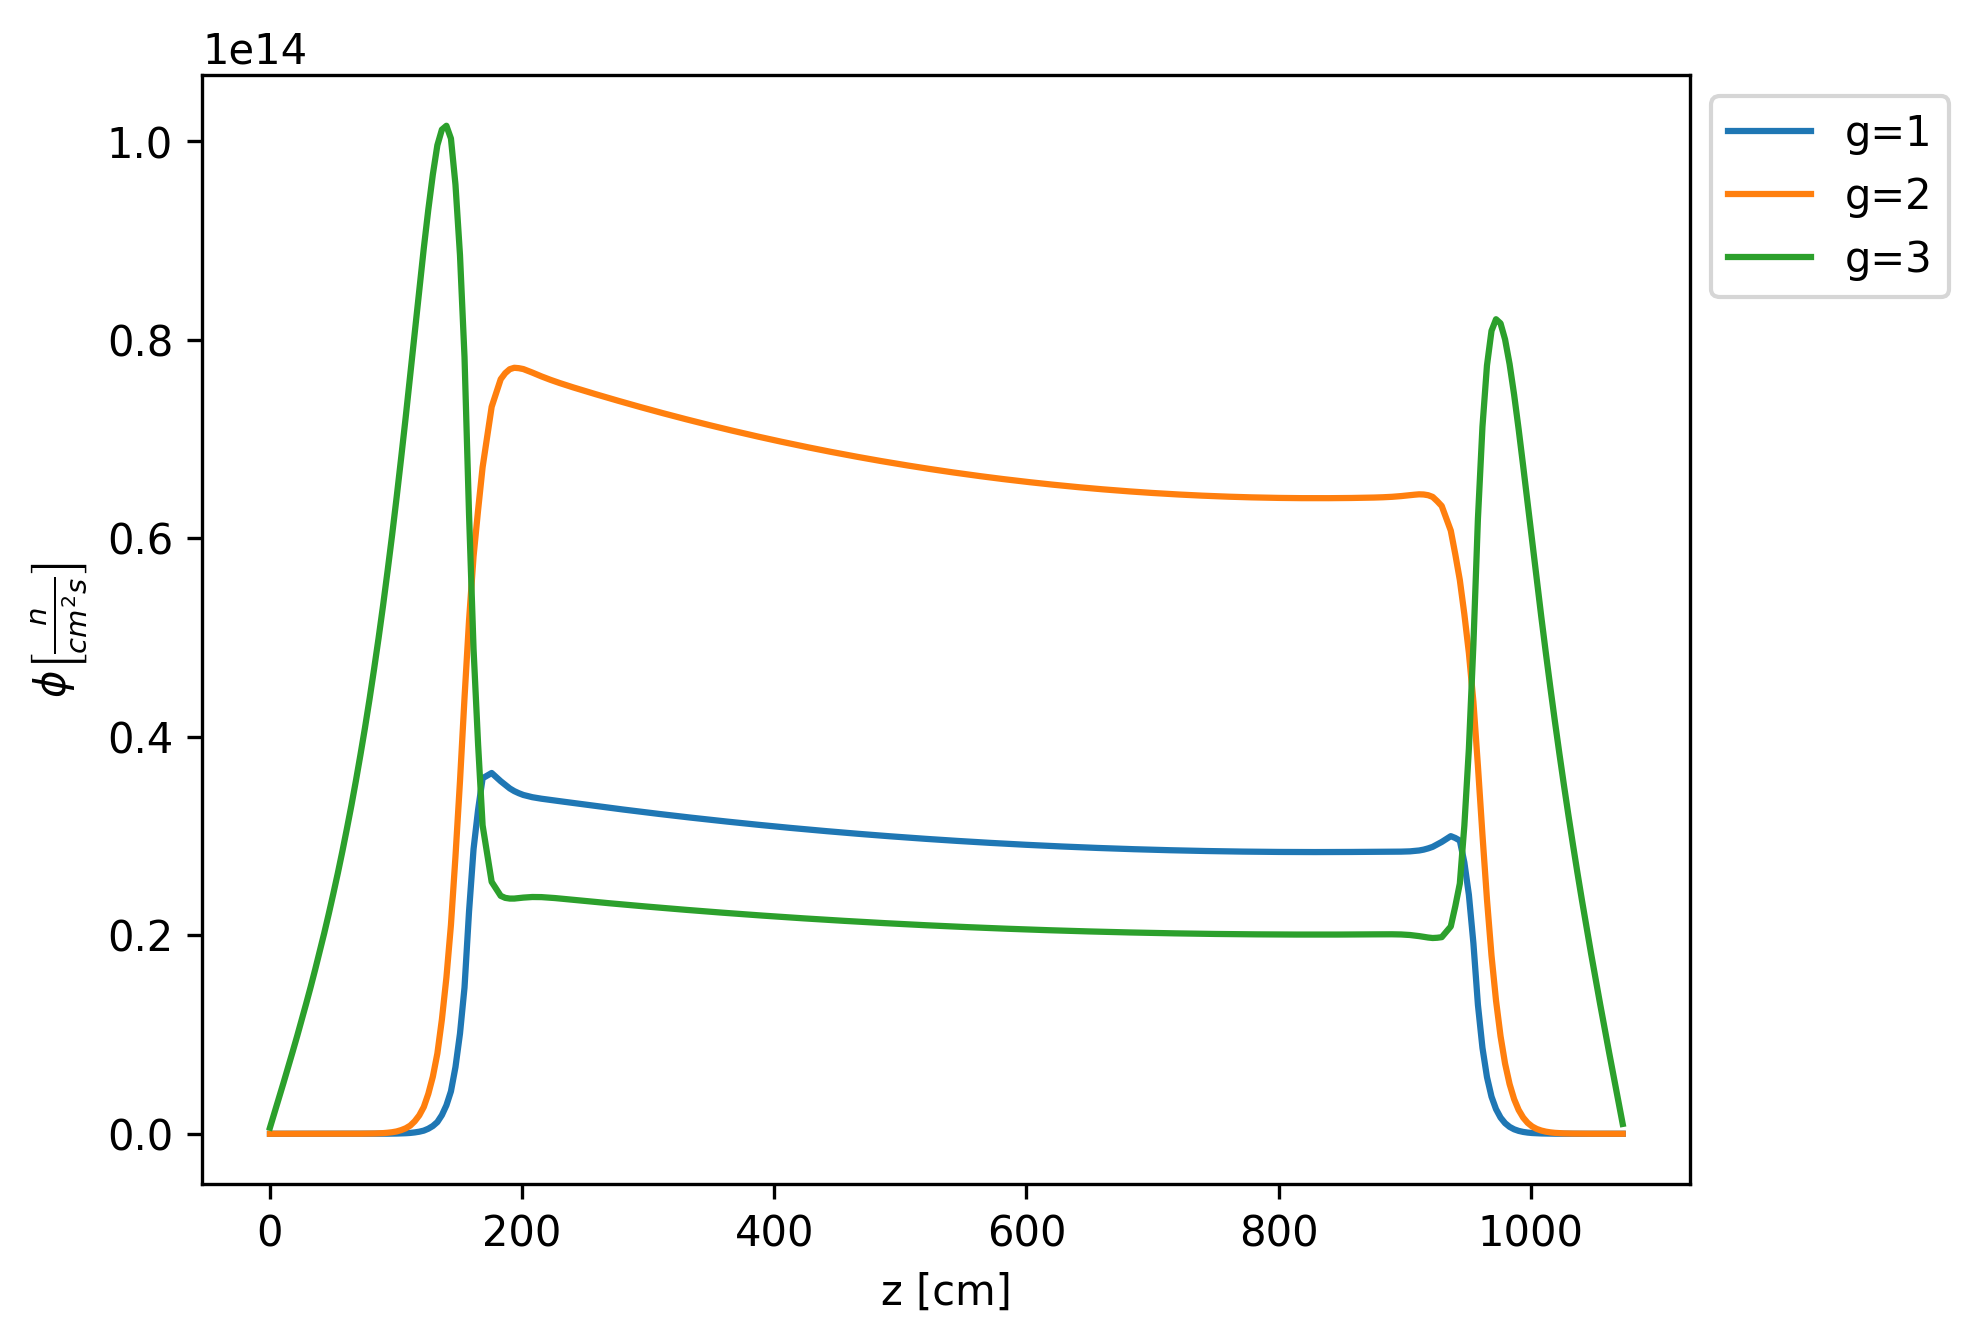
\includegraphics[width=0.45\textwidth]{figures-assembly/3D-assembly-LBP-600-26G}
    }
    \subfloat[Serpent.]{
        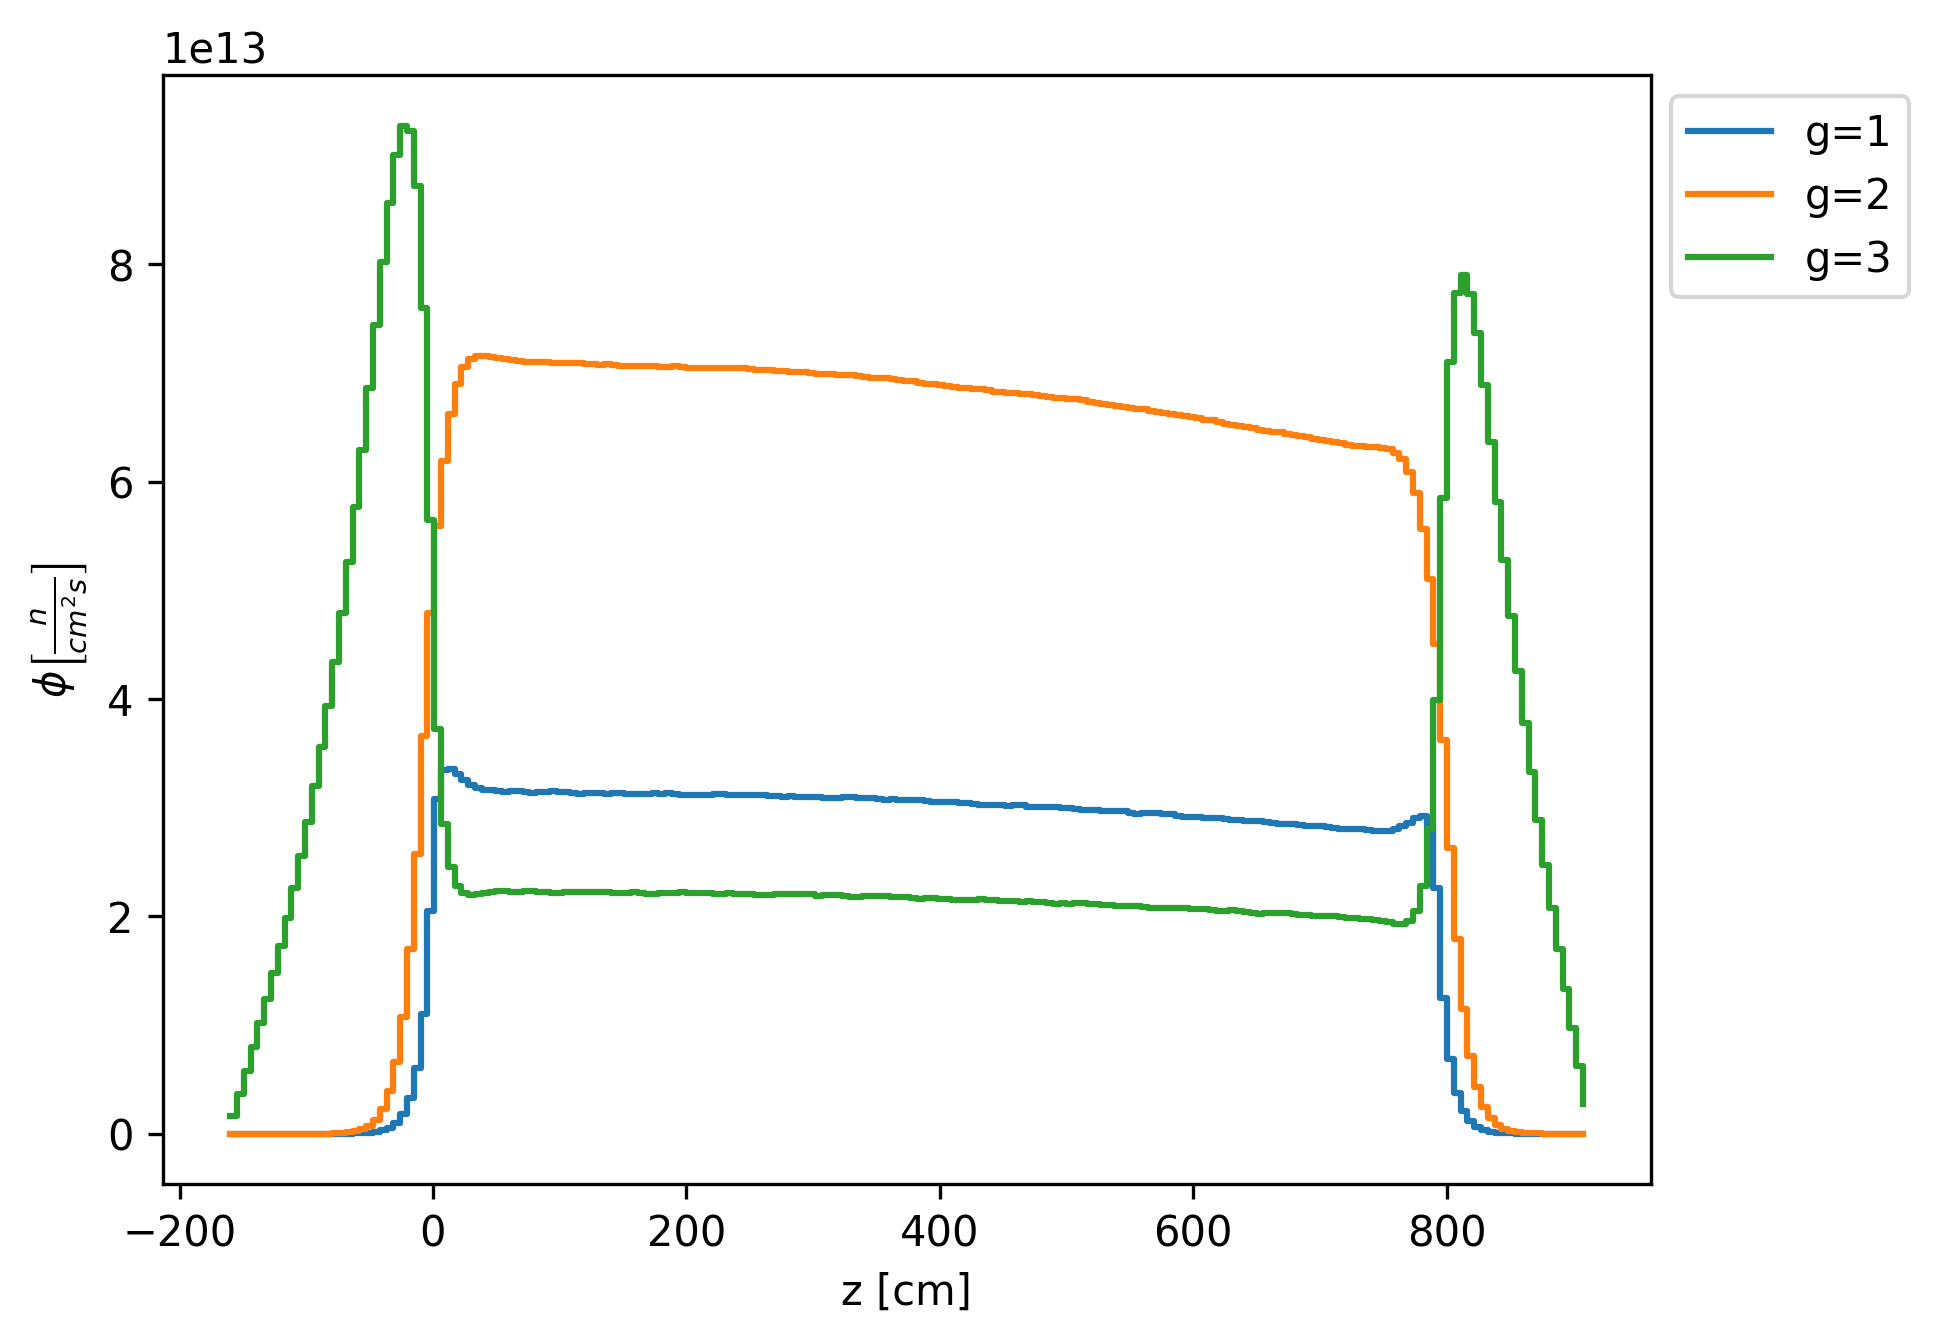
\includegraphics[width=0.45\textwidth]{figures-assembly/serpent26G-LBP-600-collapse}
    }
  \hfill
    \caption{Case LBP at 600K. 3-group axial neutron flux.}
  \label{fig:assembly-LBP-600-flux}
\end{figure}

% LBP 1200
\begin{figure}[htbp!]
  \centering
    \subfloat[Moltres.]{
        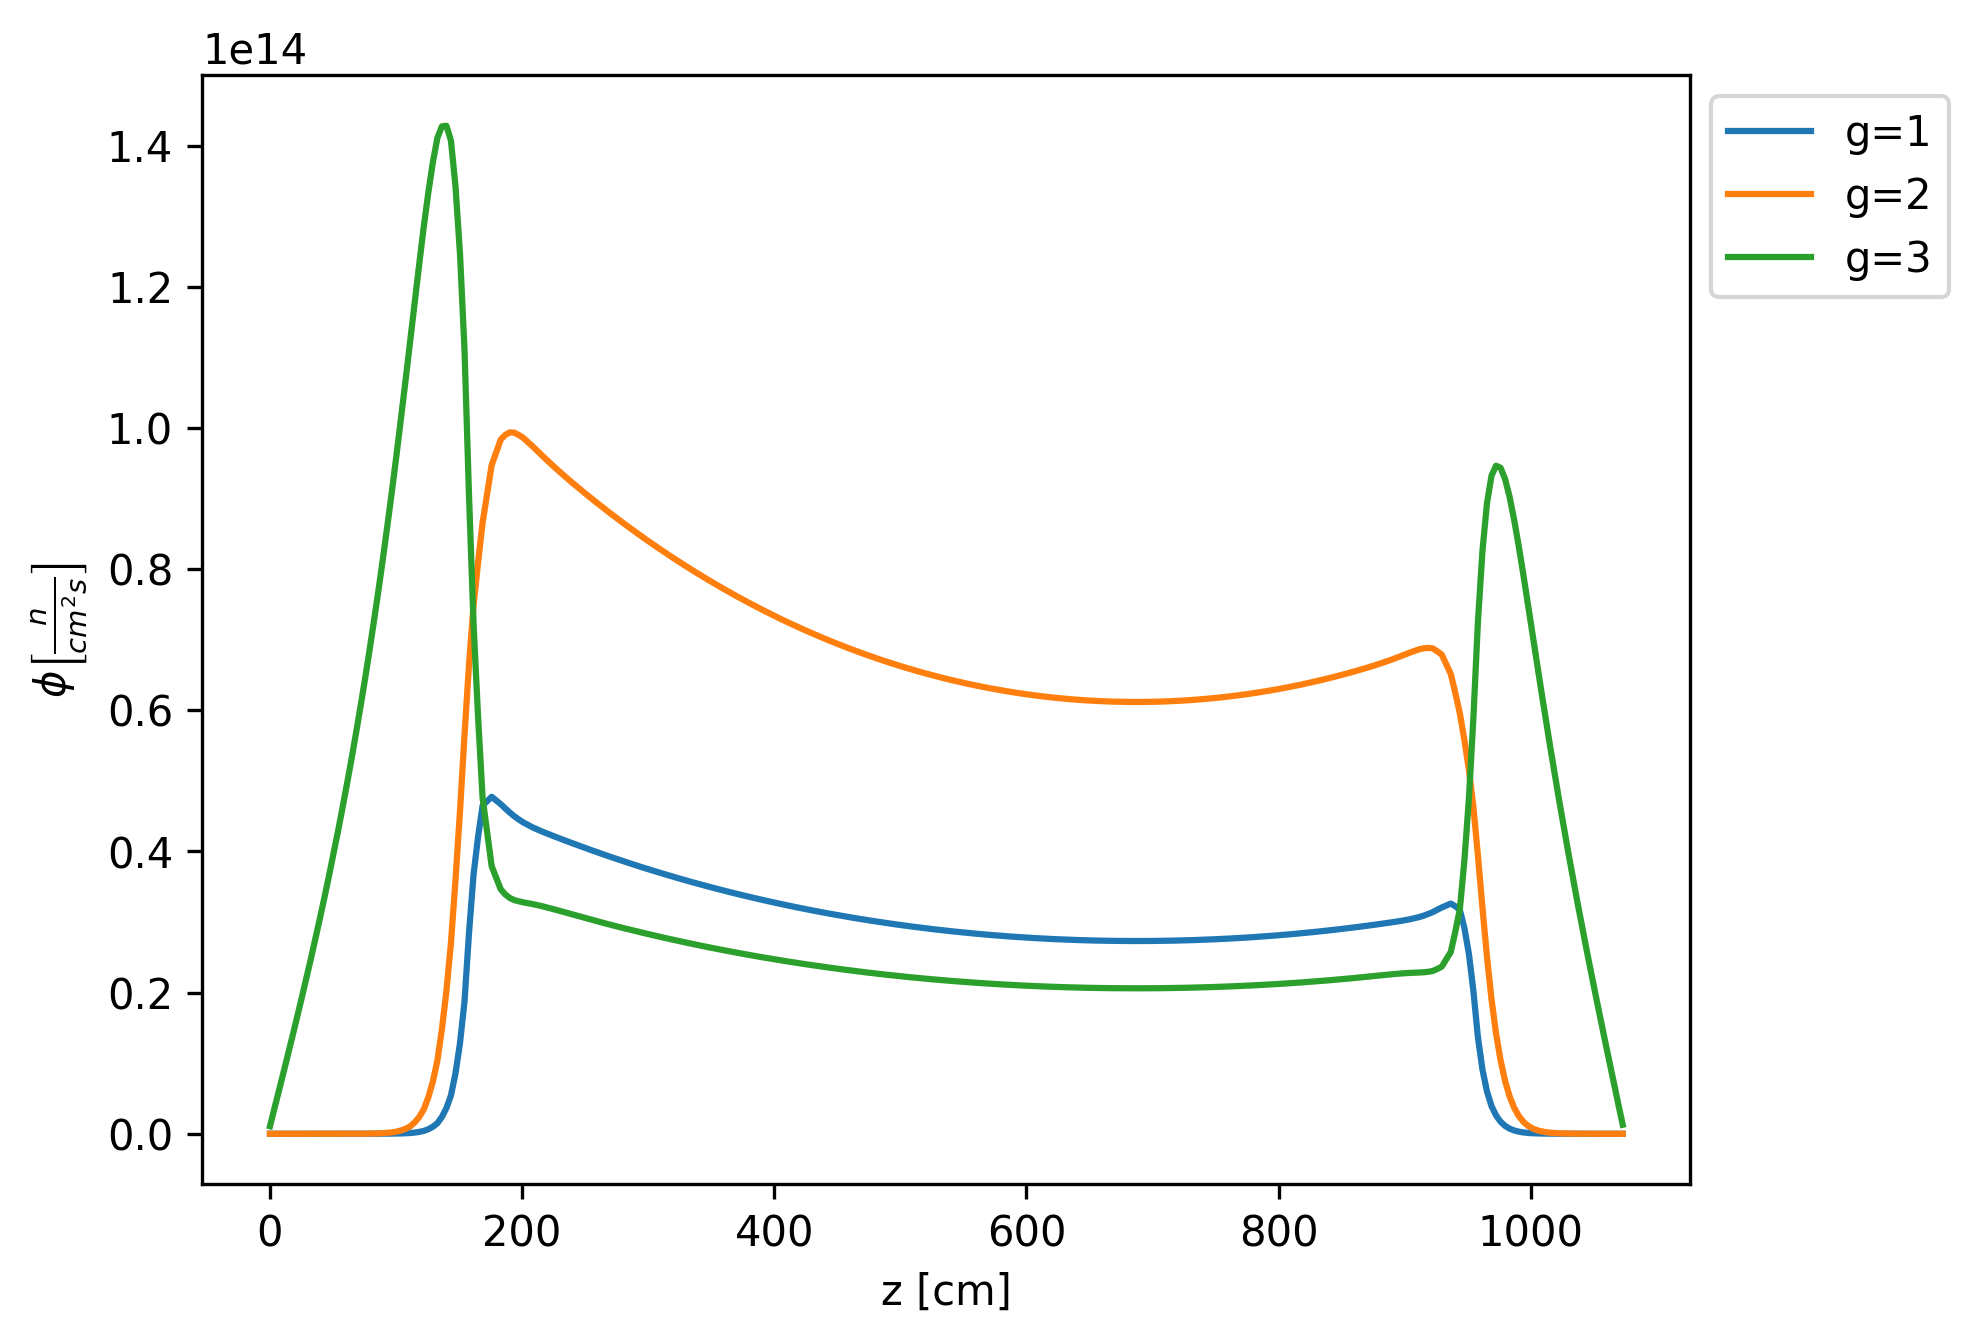
\includegraphics[width=0.45\textwidth]{figures-assembly/3D-assembly-LBP-1200-26G}
    }
    \subfloat[Serpent.]{
        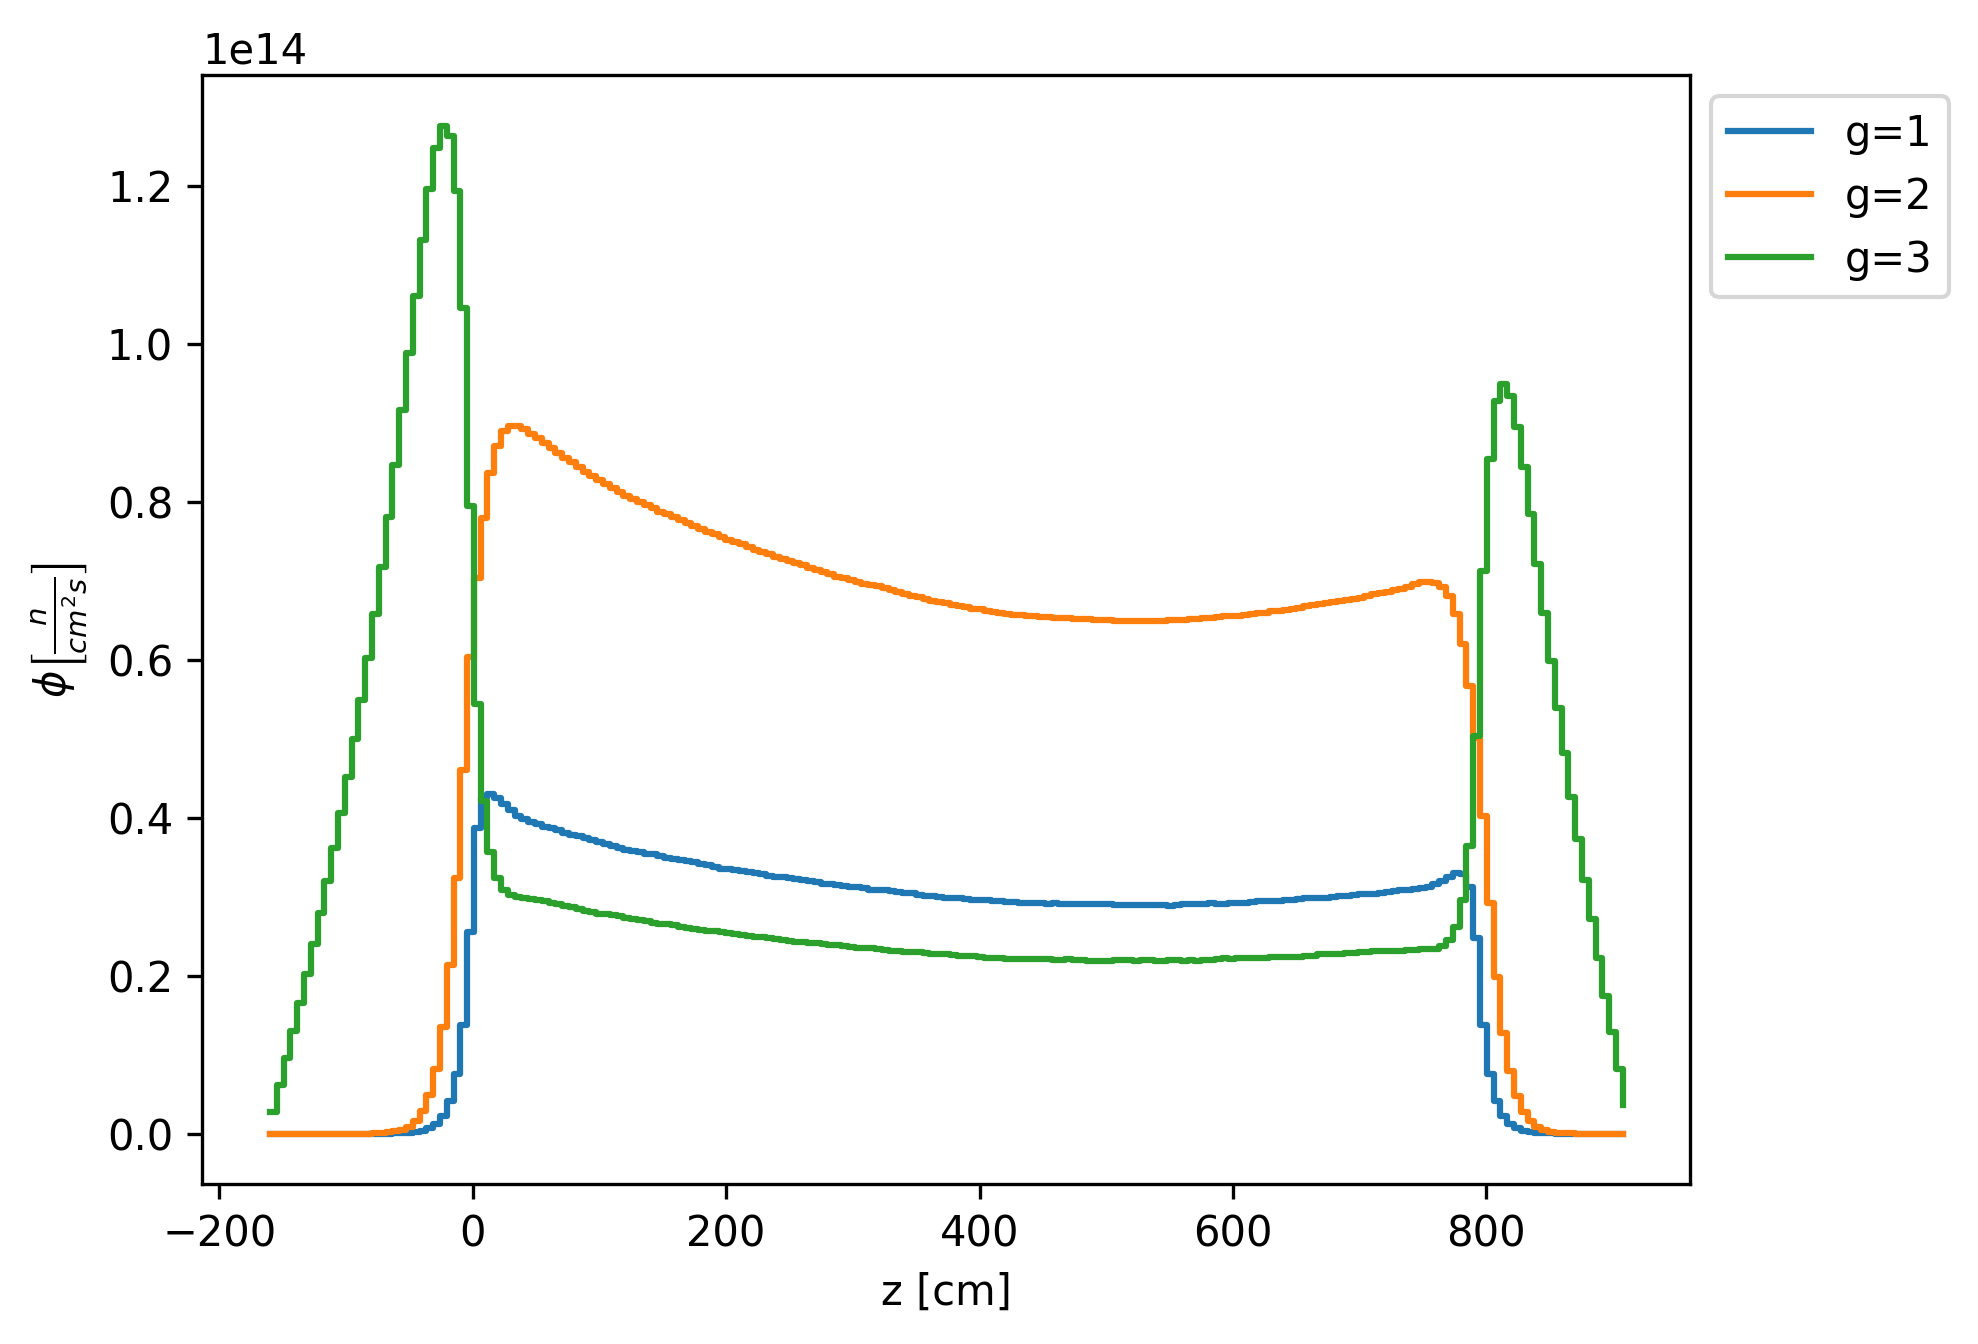
\includegraphics[width=0.45\textwidth]{figures-assembly/serpent26G-LBP-1200-collapse}
    }
  \hfill
    \caption{Case LBP at 1200K. 3-group axial neutron flux.}
  \label{fig:assembly-LBP-1200-flux}
\end{figure}

% eigenvalues
Table \ref{tab:keff} exhibits the reactivity difference ($\Delta \rho$) between the Serpent and Moltres eigenvalues.
We used equation \ref{eq:delta-rho} to obtain $\Delta \rho$.
The eigenvalues in Moltres differ slightly from the eigenvalues in Serpent.
Overall, the reactivity difference is less than 50 pcm.
We note that the number of energy groups does not affect the accuracy of the eigenvalue calculations in Moltres.

\begin{align}
	\Delta \rho &= \left| \frac{k_1-k_2}{k_1 k_2} \right| \label{eq:delta-rho}
  \intertext{where}
  k_1 &= \mbox{Serpent eigenvalue} \notag \\
  k_2 &= \mbox{Moltres eigenvalue.} \notag
\end{align}

\begin{table}[htbp!]
  \centering
  \caption{Serpent and Moltres eigenvalues.}
  \begin{tabular}{l|l|llllllll}
  \toprule
              & Serpent 					& \multicolumn{8}{c}{$\Delta \rho$ [pcm]}            \\ \cline{3-10} 
              &              			& 3   & 6   & 9   & 12   & 15   & 18   & 21   & 26   \\
  \midrule
no LBP, 600K  & 1.43800           & 10  & 7   & 6   & 6    & 5    & 6    & 6    & 12   \\
no LBP, 1200K & 1.37771           & 23  & 15  & 4   & 3    & 2    & 2    & 1    & 11   \\
LBP, 600K     & 1.12861           & 44  & 21  & 24  & 25   & 25   & 24   & 19   & 9    \\
LBP, 1200K    & 1.06554           & 36  & 40  & 29  & 32   & 44   & 43   & 25   & 25   \\
  \bottomrule
  \end{tabular}
  \label{tab:keff}
\end{table}

Figures \ref{fig:assembly-noLBP-er} and \ref{fig:assembly-LBP-er} show the $L_2$-norm of the relative error for the different energy group structures.
The no LBP case's relative error is smaller than the LBP case's relative error.
Overall, the relative error decreases with an increase in the number of energy groups.
Nonetheless, this is not always the case.
For example, in Figure \ref{fig:assembly-noLBP-er-b}, going from 12 to 15 groups, the thermal flux improves, but the fast flux worsens.
Additionally, we observe that a low number of energy groups yields more than 100$\%$ error.
In which case, we can conclude that the solution is wrong.

% No LBP
\begin{figure}[htbp!]
	\centering
    \subfloat[600K.]{
        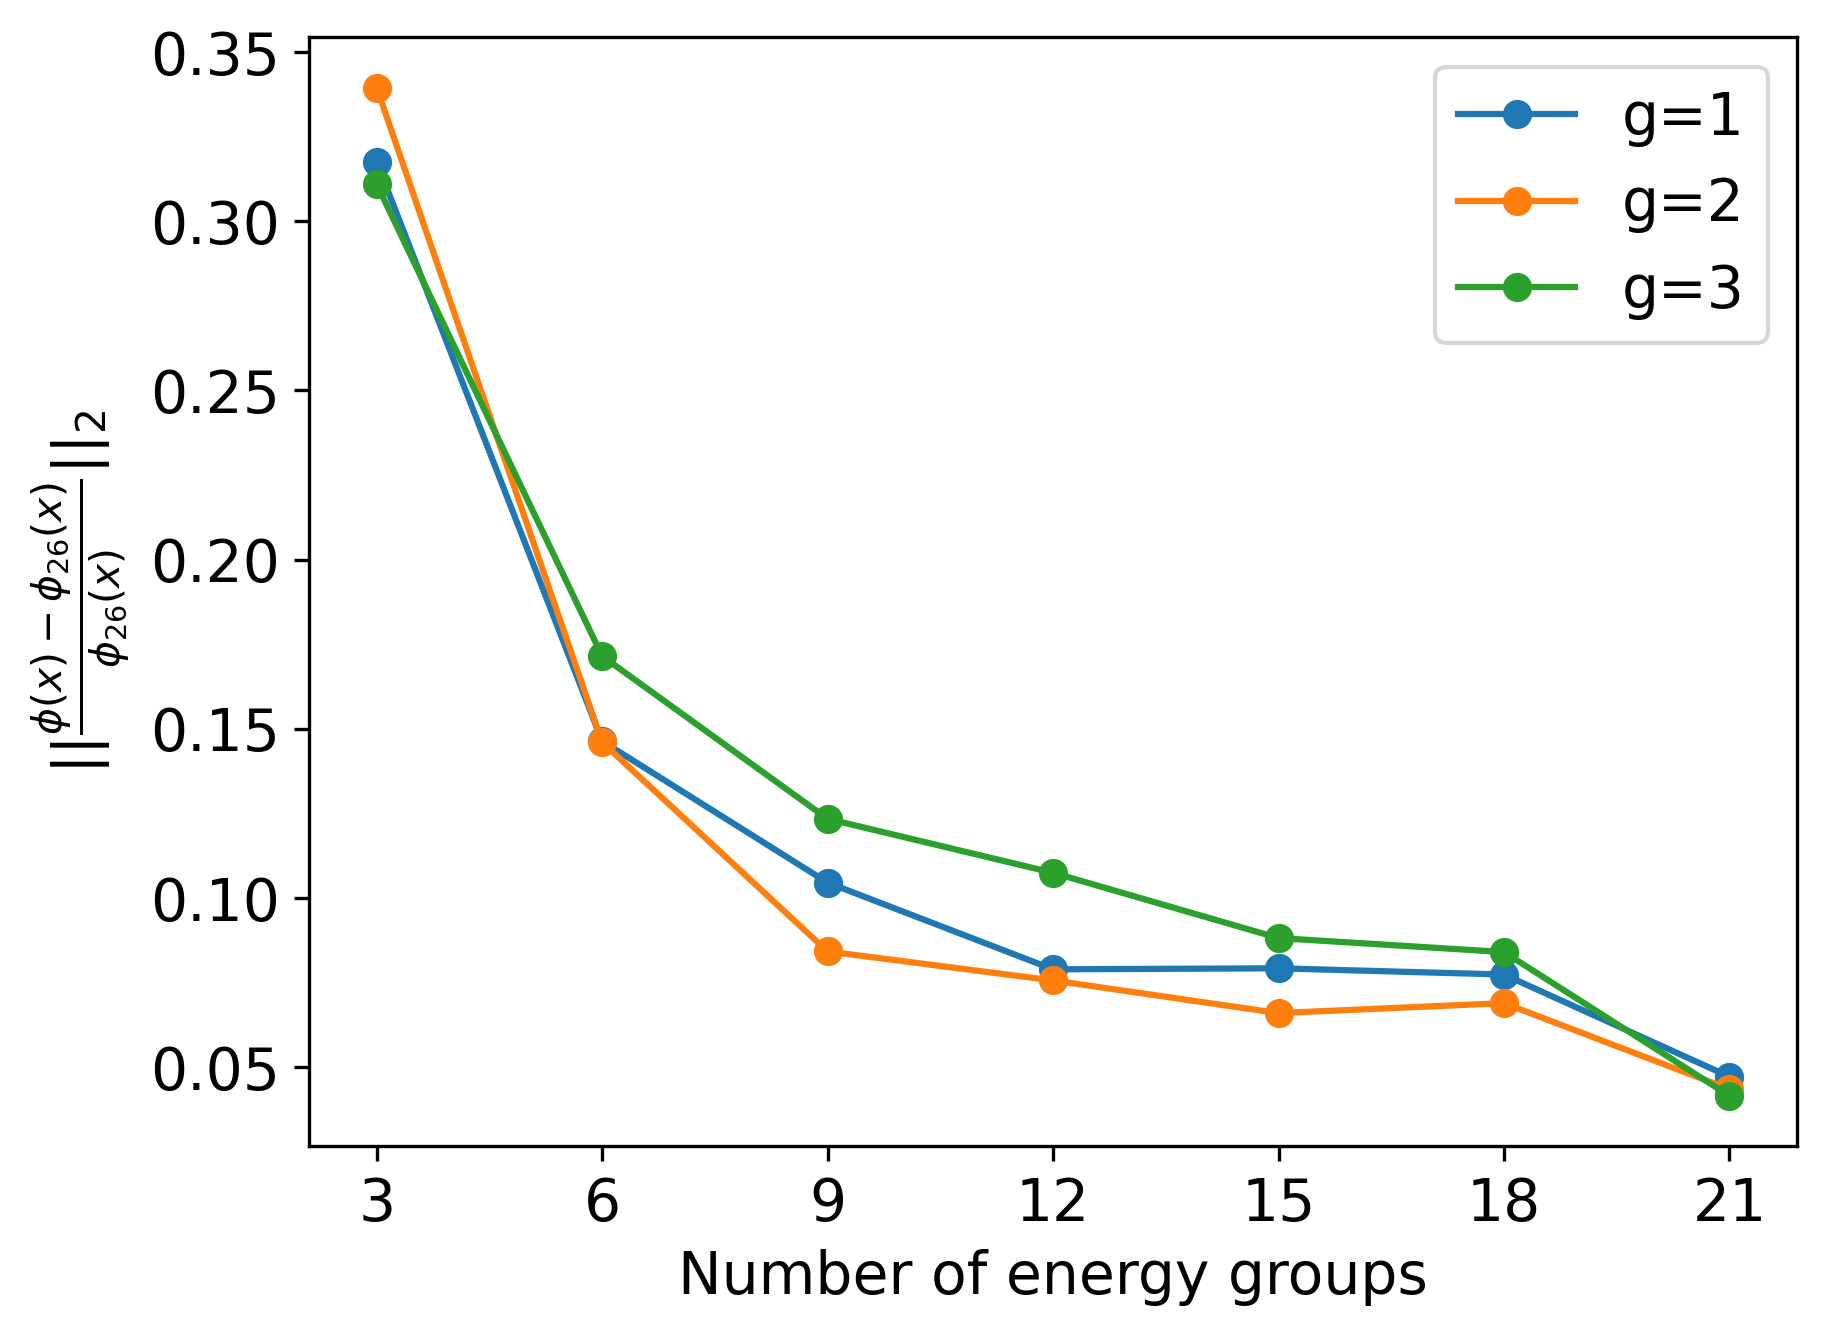
\includegraphics[width=0.45\textwidth]{figures-assembly/noLBP-600-er-final}
    }
    \subfloat[1200K.\label{fig:assembly-noLBP-er-b}]{
        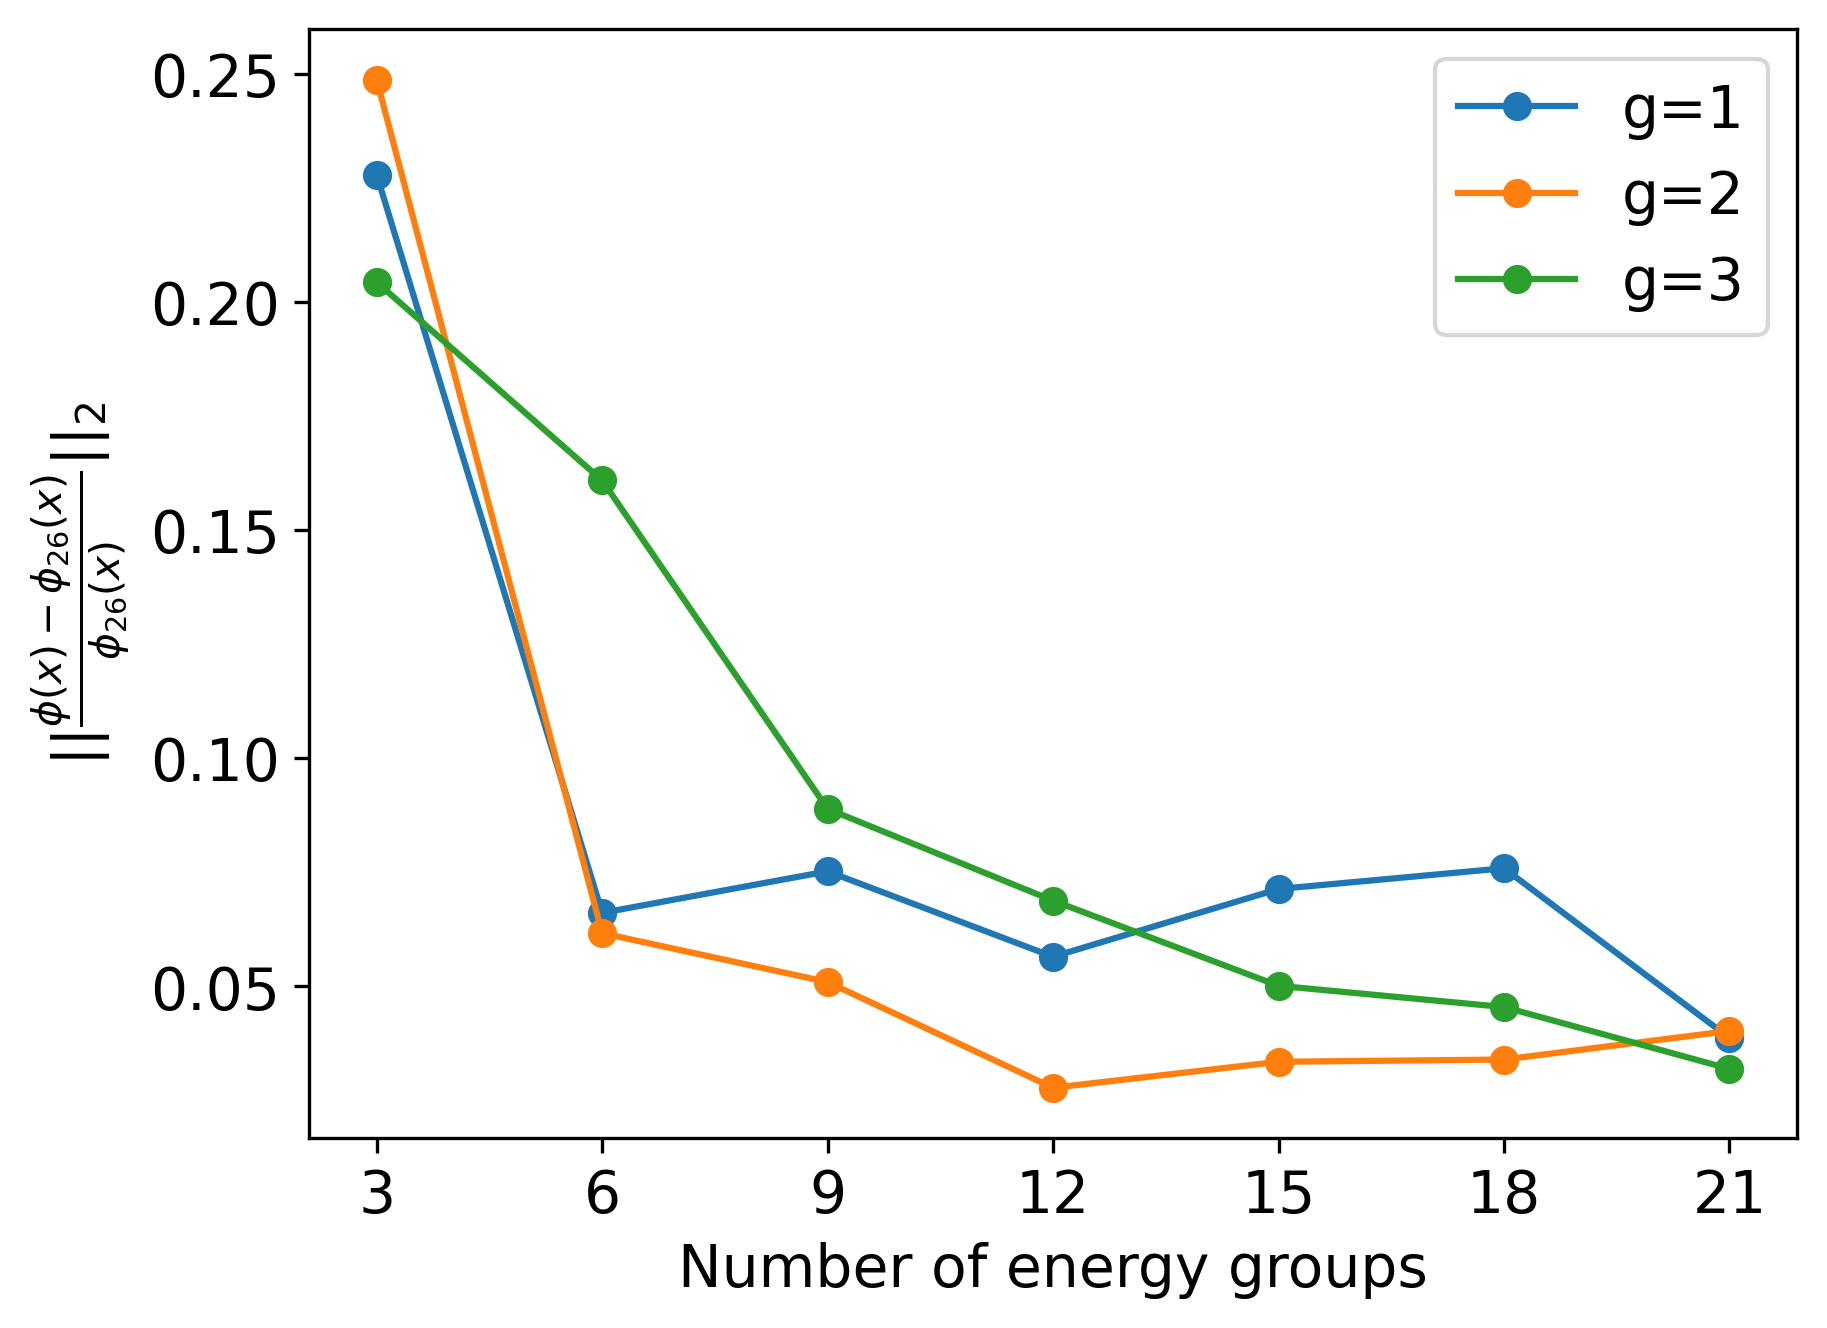
\includegraphics[width=0.45\textwidth]{figures-assembly/noLBP-1200-er-final}
    }
	\hfill
    \caption{No LBP case. L$_2$-norm relative error for different number of energy group structures.}
	\label{fig:assembly-noLBP-er}
\end{figure}

% LBP
\begin{figure}[htbp!]
	\centering
    \subfloat[600K.]{
        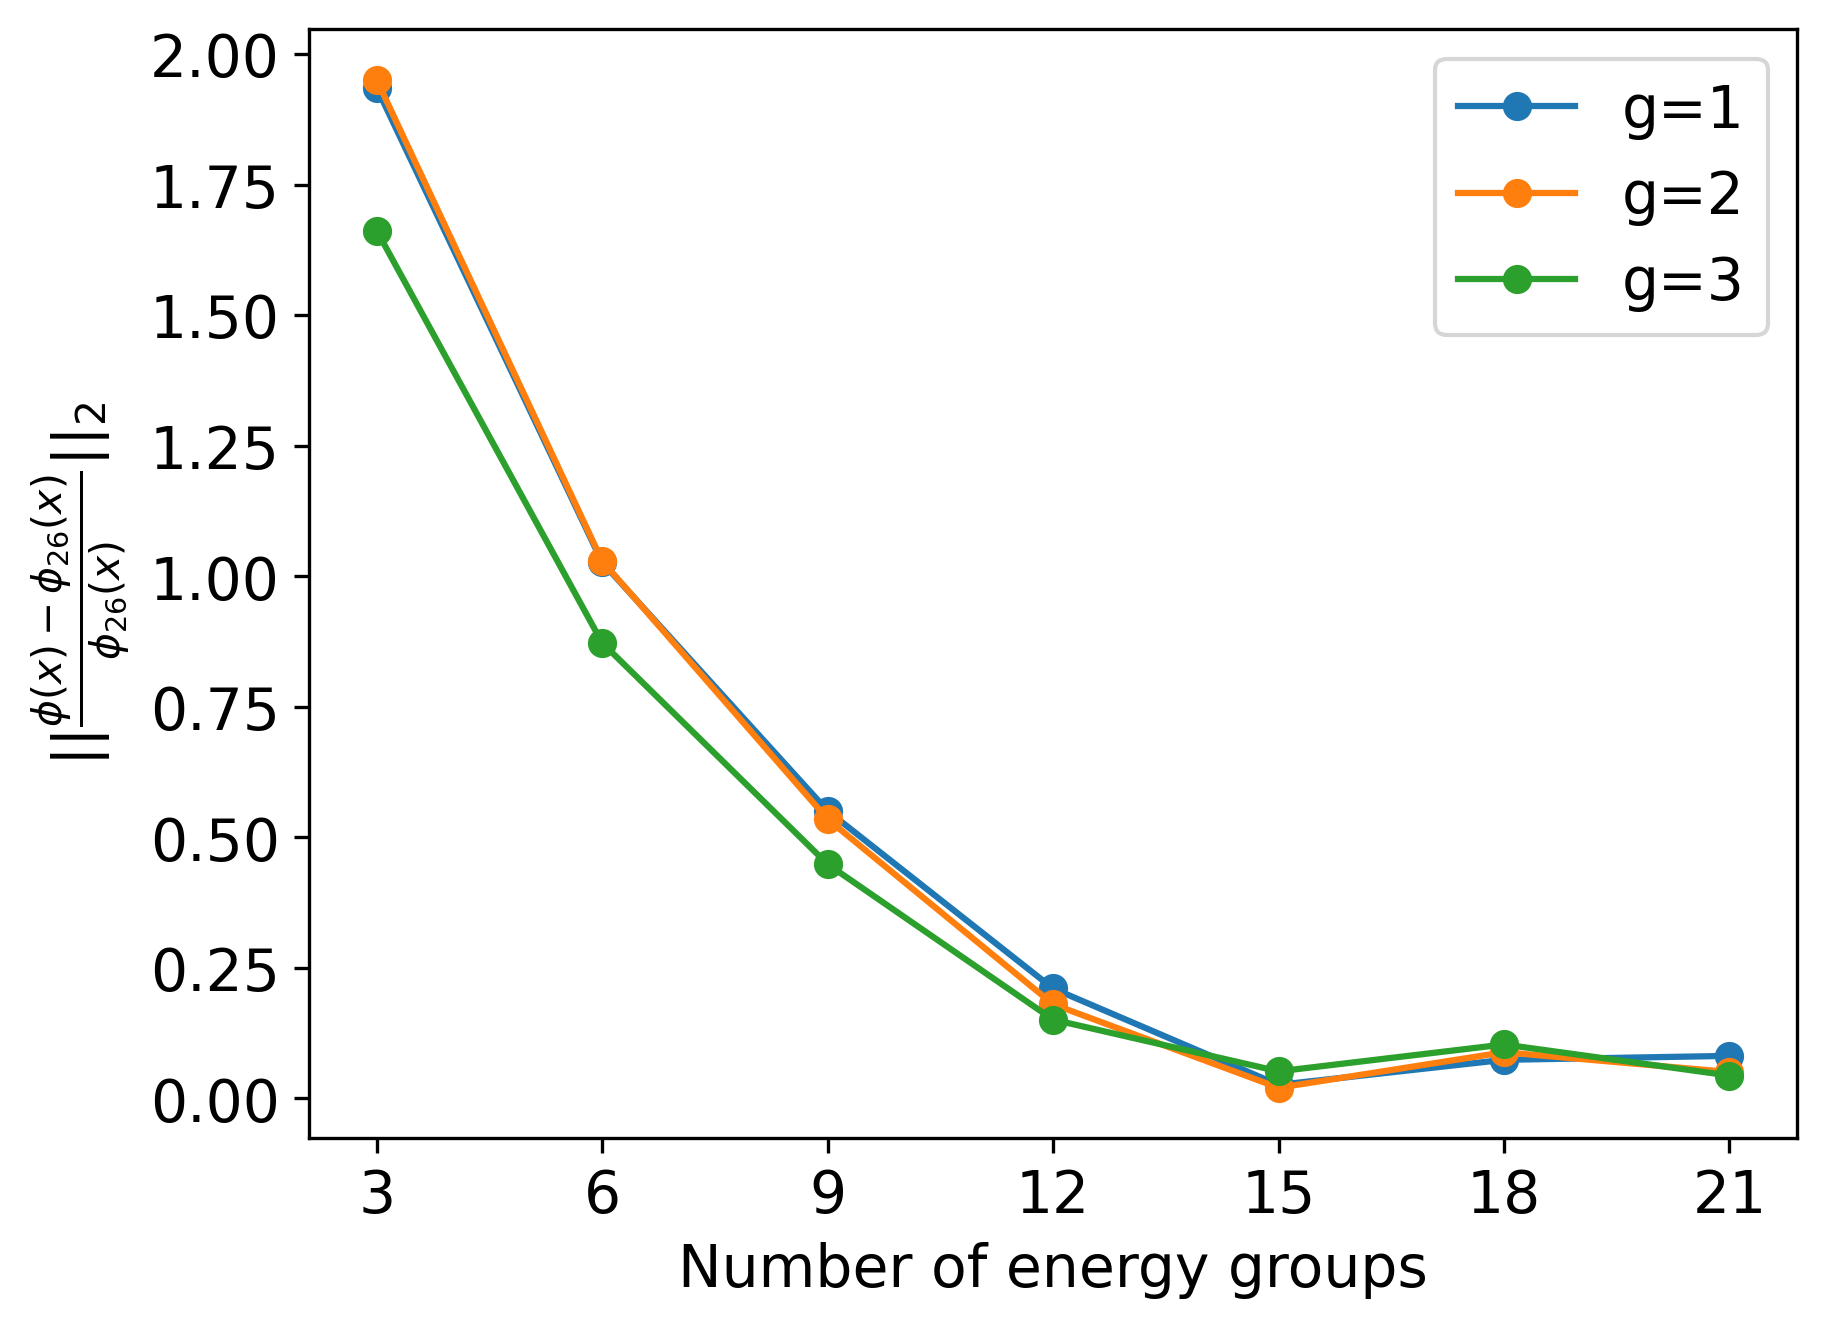
\includegraphics[width=0.45\textwidth]{figures-assembly/LBP-600-er-final}
    }
    \subfloat[1200K.]{
        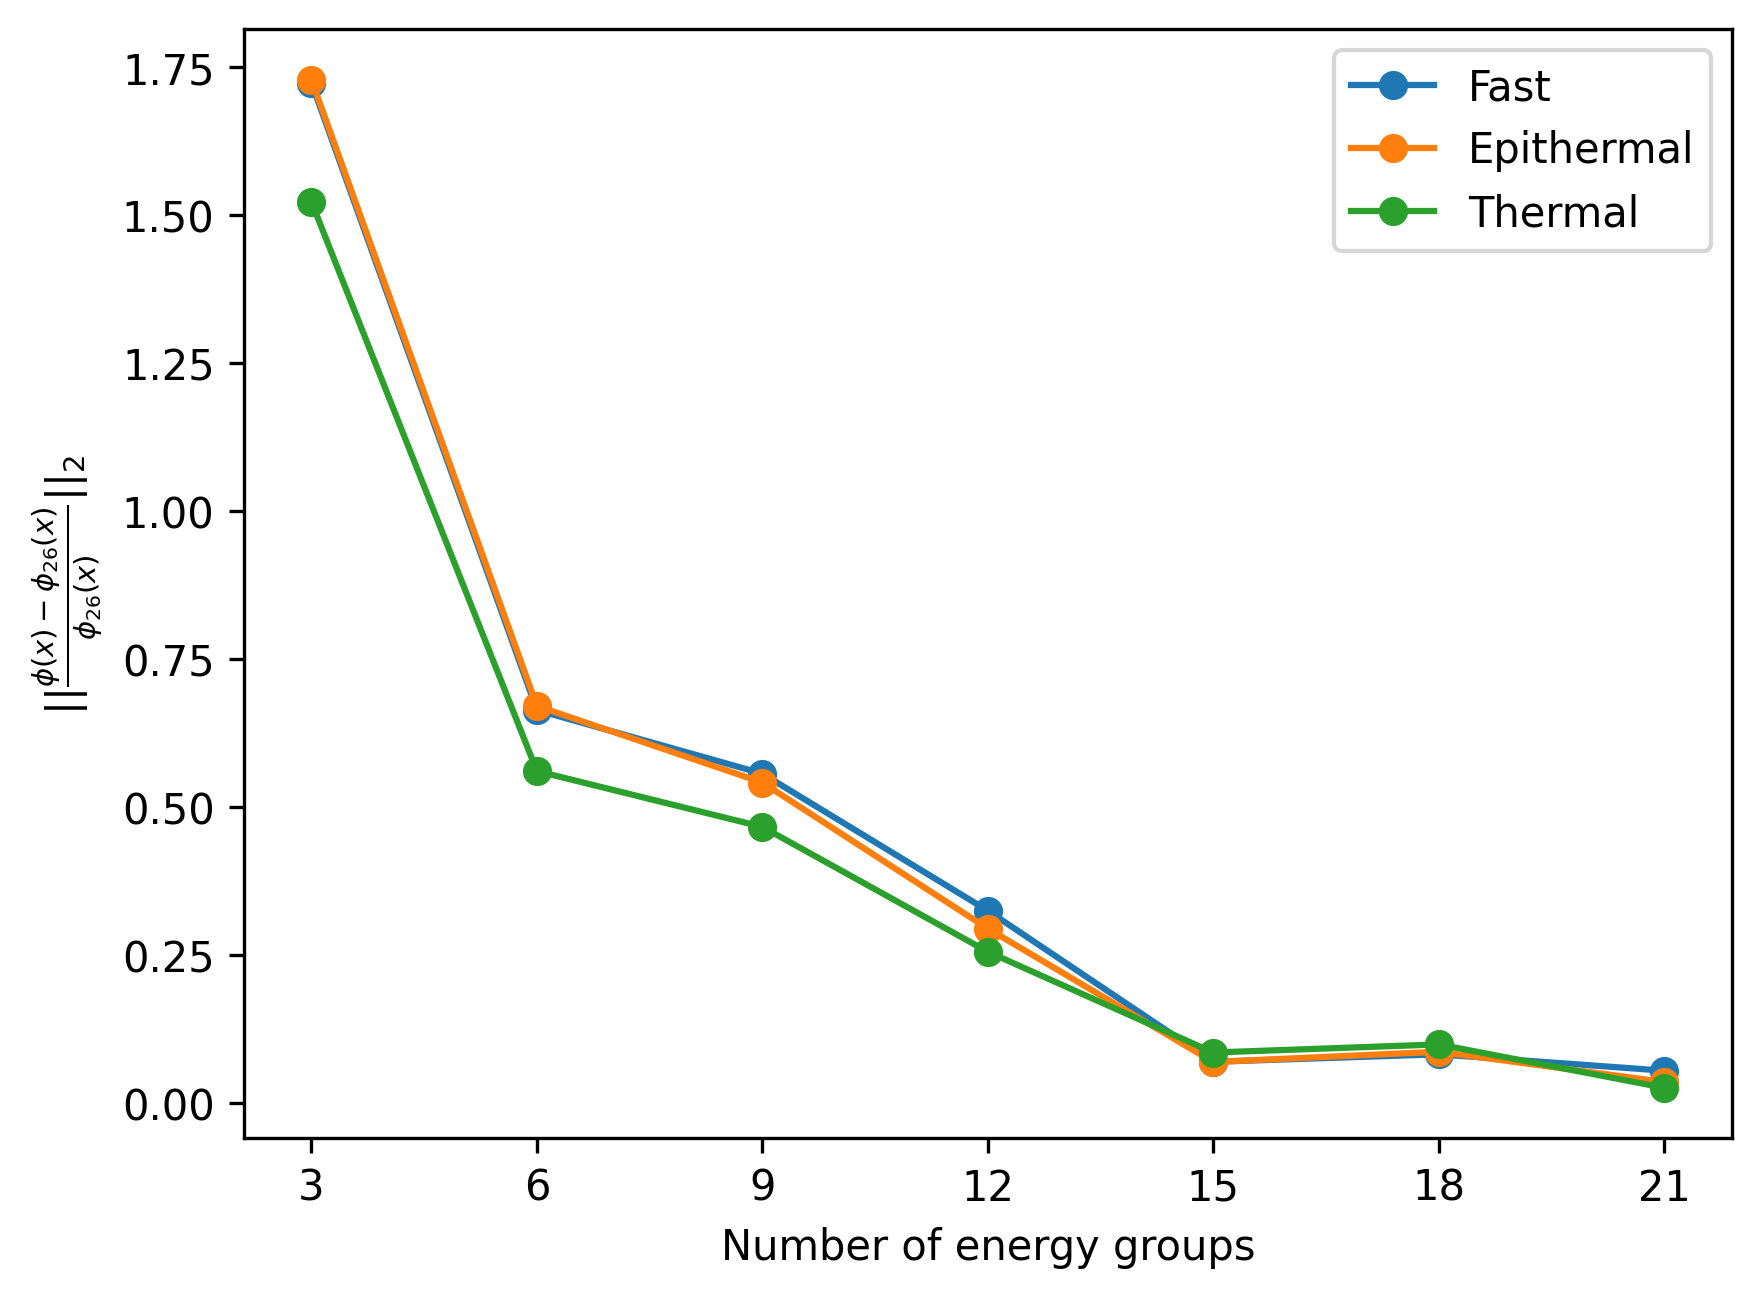
\includegraphics[width=0.45\textwidth]{figures-assembly/LBP-1200-er-final}
    }
	\hfill
    \caption{LBP case. L$_2$-norm relative error for different number of energy group structures.}
	\label{fig:assembly-LBP-er}
\end{figure}

We added to the analysis the computational time and the peak memory usage during the simulations, Figure \ref{fig:assembly-time}.
All the simulations used 128 cores.
We present only the cases at 600K because the impact of the temperature change was not significant.
The computational requirements rise with an increase in the number of energy groups.
As the geometry uses a constant number of elements, the DoFs/energy-group is constant for all the simulations.
Thus, the total number of DoFs is proportional to the number of energy groups.
We also discern that the overall time of the LBP cases is higher than the no LBP cases.

% Time and memory
\begin{figure}[htbp!]
	\centering
    \subfloat[No LBP and 600 K.]{
        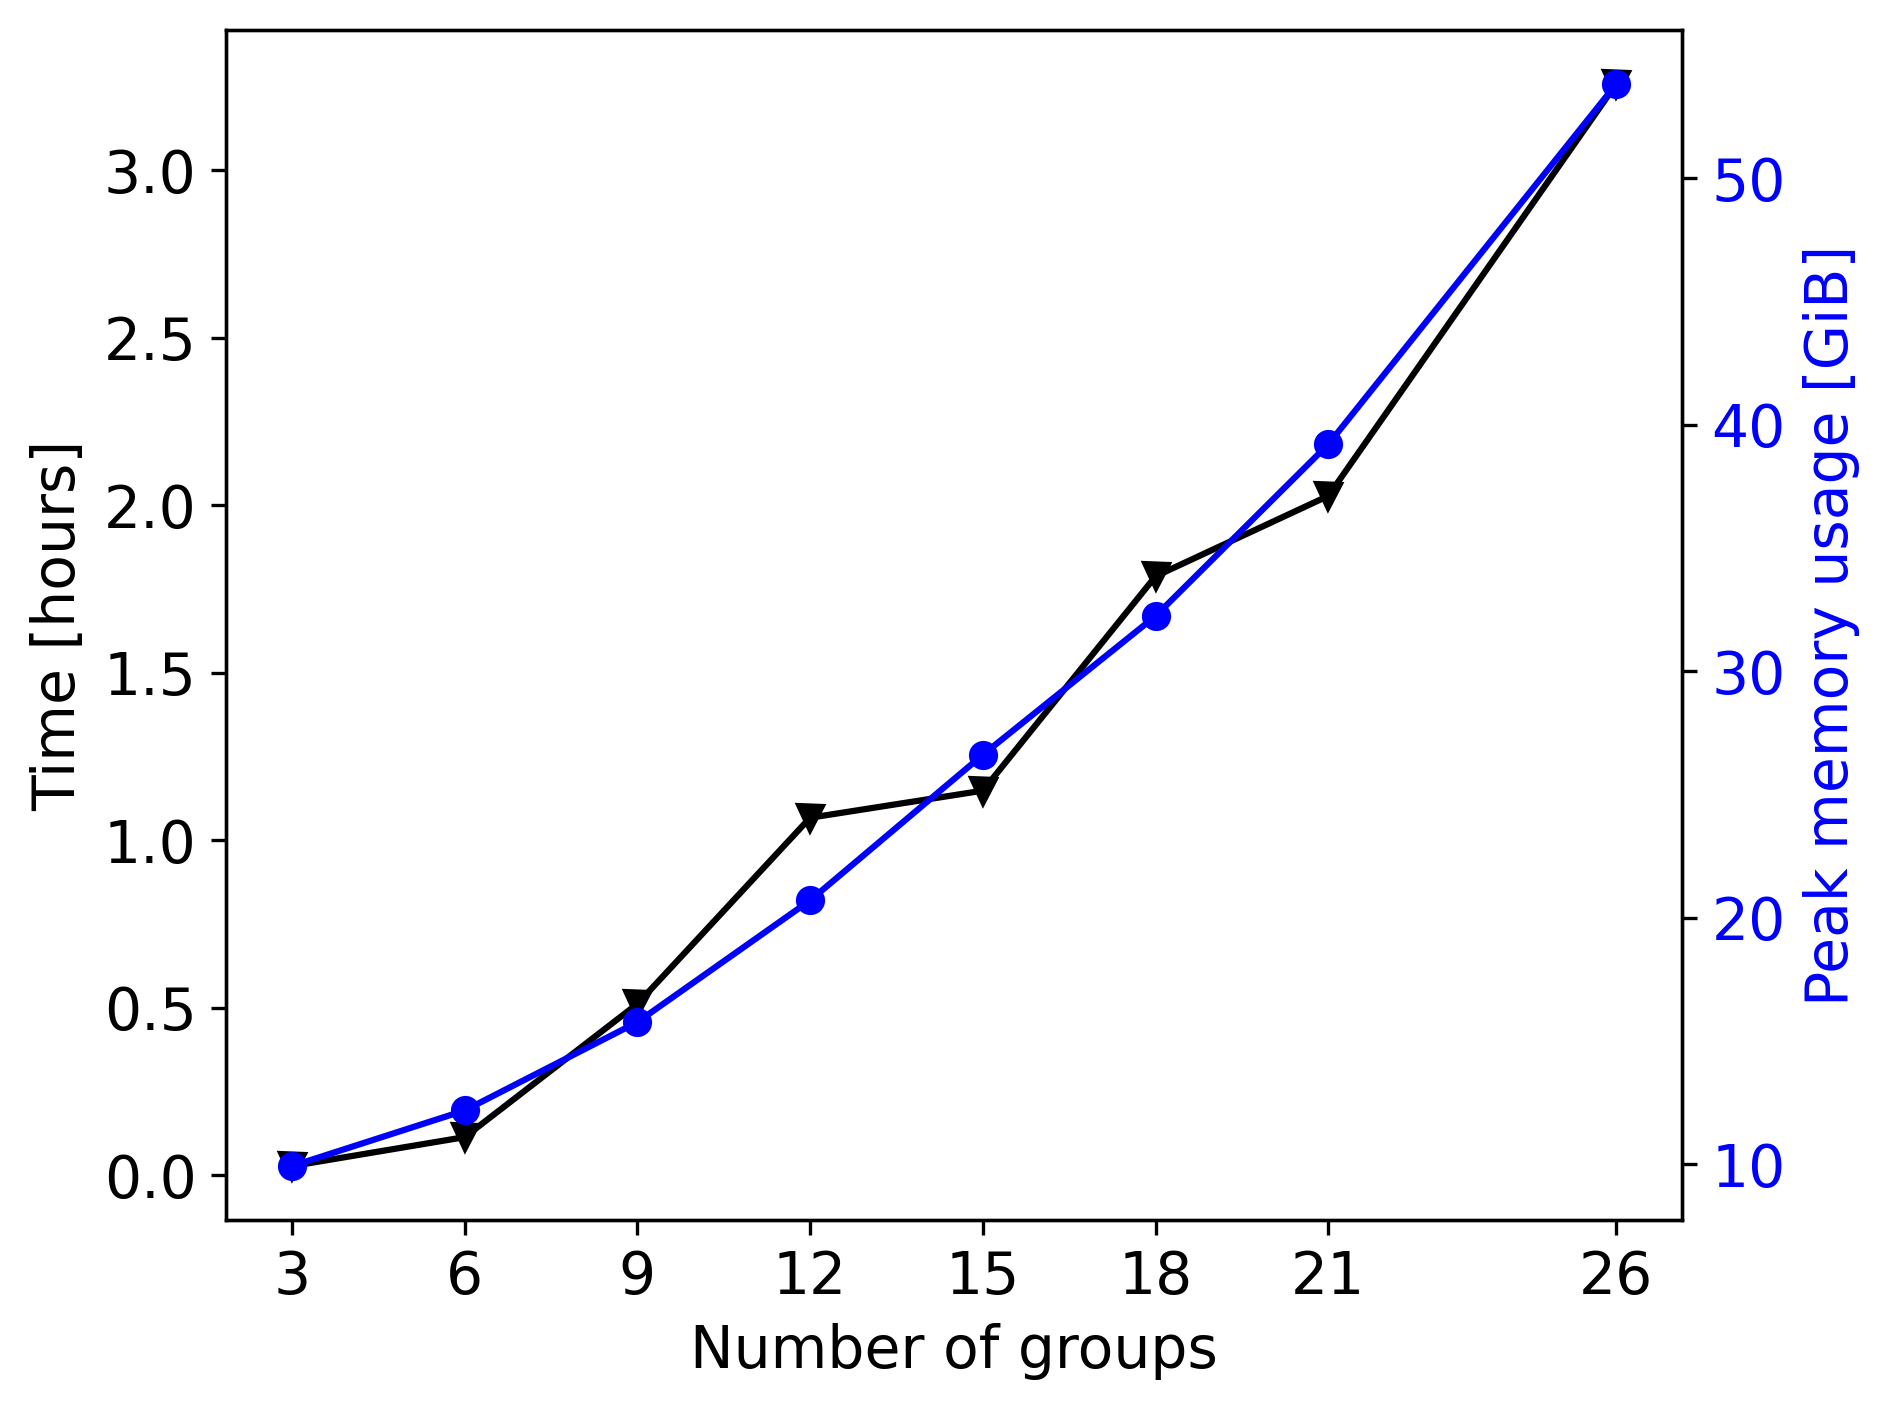
\includegraphics[width=0.45\textwidth]{figures-assembly/time-noLBP-600}
    }
    \subfloat[LBP and 600 K.]{
        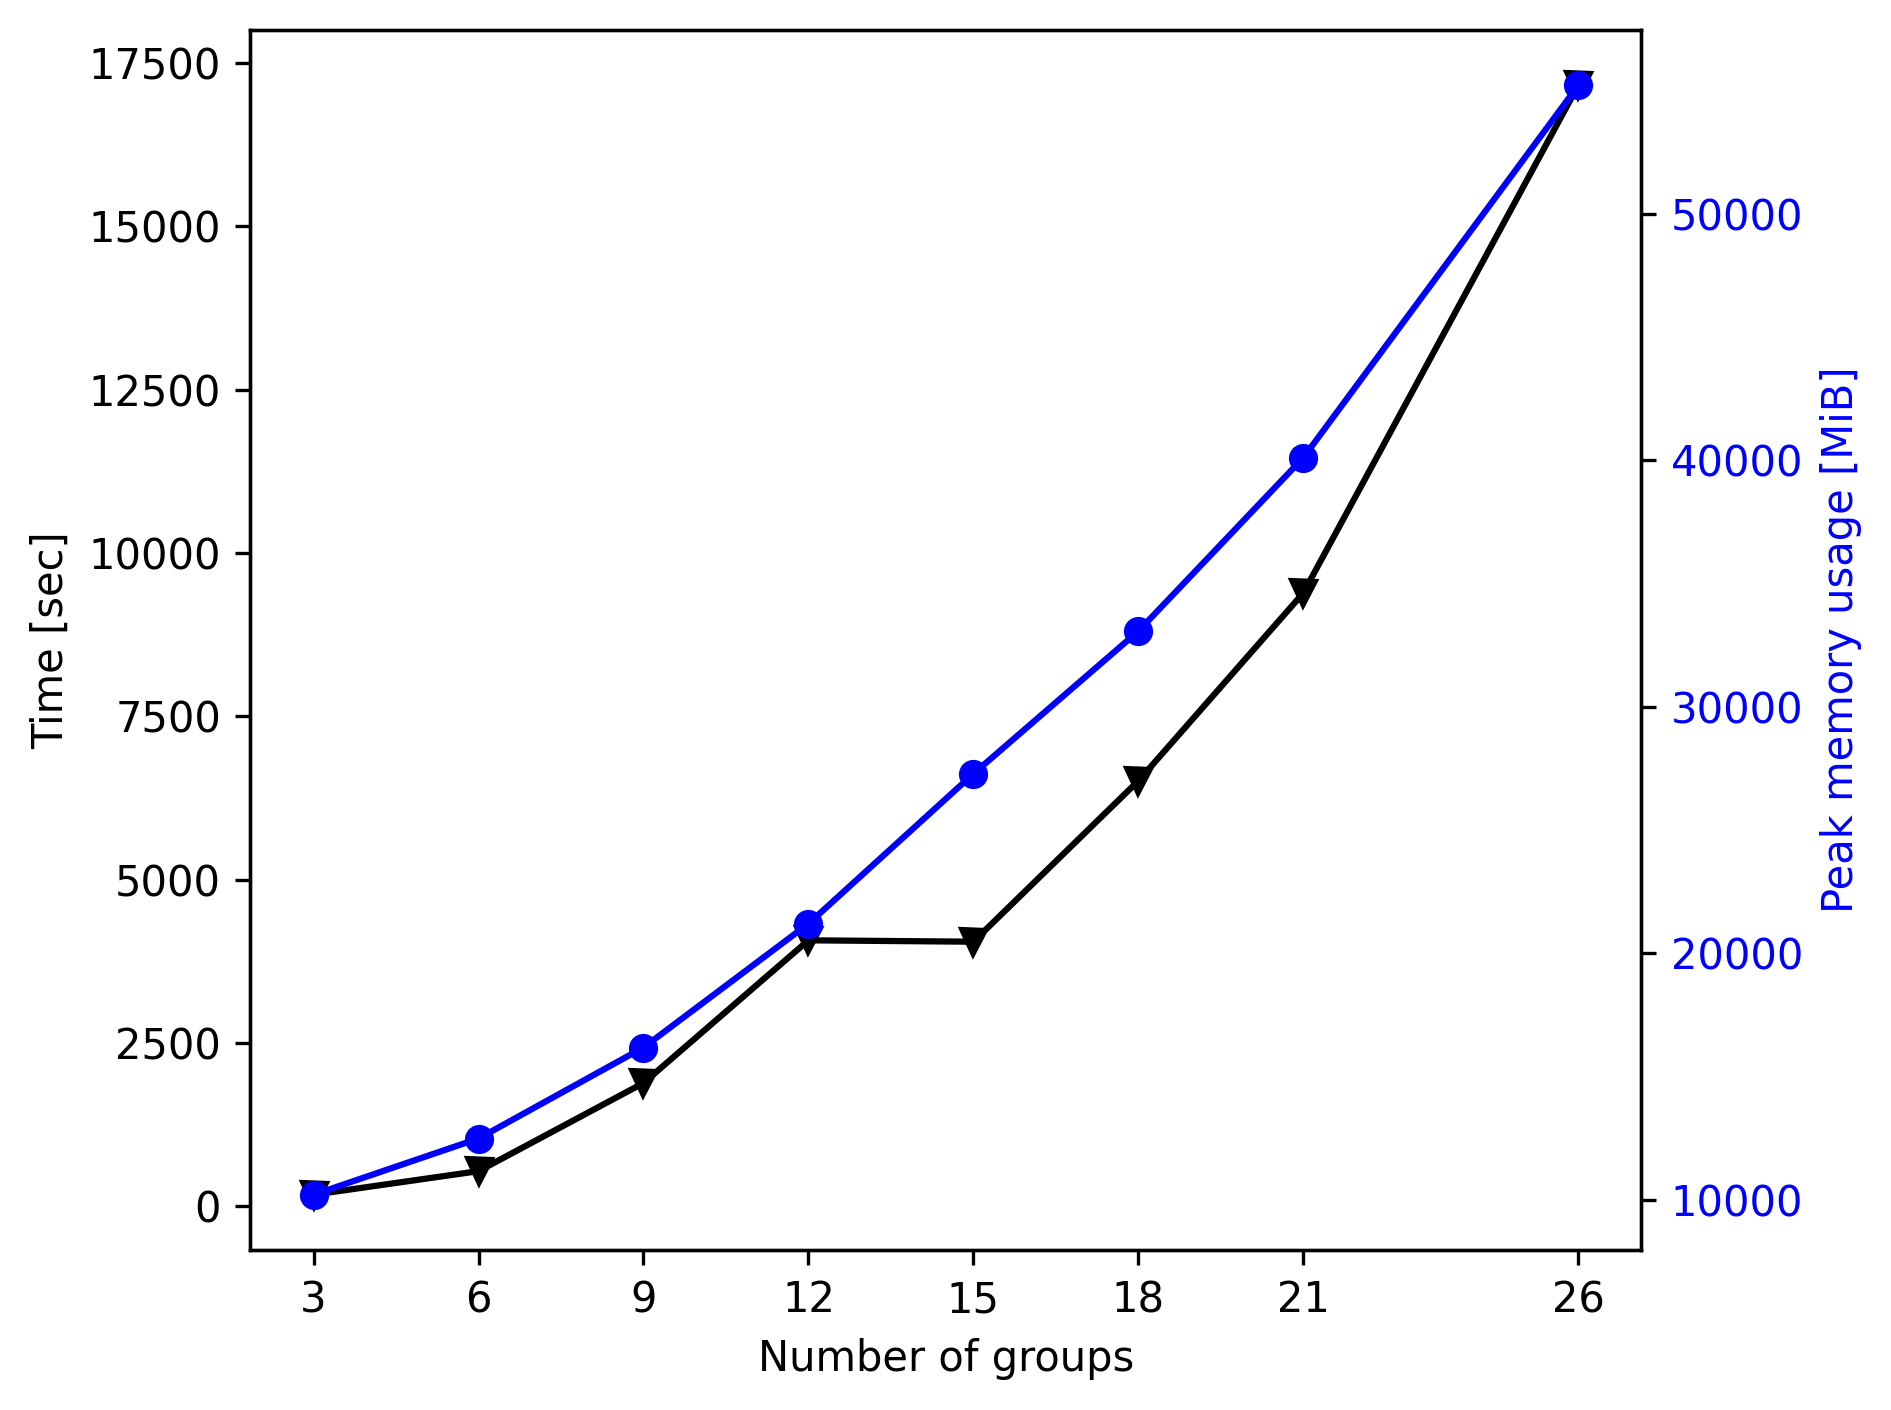
\includegraphics[width=0.45\textwidth]{figures-assembly/time-LBP-600}
    }
	\hfill
	\caption{Computational time and memory requirements for different number of energy group structures.}
	\label{fig:assembly-time}
\end{figure}

Finally, we analyzed the impact of changing the energy group structure for a constant number of energy groups.
We chose 15 energy groups, as it yields a good overall accuracy and a not so high computational expense.
Table \ref{tab:energygroups} holds the different energy group structures.
Table \ref{tab:accuracy15} exhibits the $L_2$-norm of the relative error for the different energy group structures.
The energy group structure has an impact on accuracy.
Some energy group structures yield better results for some cases while giving worse results for others.
For example, the structure $15d$ gives better results for the LBP at 600K case than for the no LBP case at 600K.
To choose the best performing structure, we used a weighted average for the different groups.
We arbitrarily chose the weights to be 0.5, 0.3, and 0.2 for the thermal, epithermal, and fast fluxes.
Using this averaging scheme, we determined the group structure $15d$ to be the best one.

\begin{table}[htbp!]
  \centering
  \caption{Axial flux relative error $L_2$-norm for various energy group structures. Values expressed in percentage.}
  \begin{tabular}{@{}l|l|l| S[table-format=2.1] S[table-format=2.1] S[table-format=2.1] S[table-format=2.1] S[table-format=2.1] }
  \toprule
	LBP                  & Temperature {[}K{]}   & Flux       & \multicolumn{1}{c@{}}{15a} & \multicolumn{1}{c@{}}{15b}  & \multicolumn{1}{c@{}}{15c}  & \multicolumn{1}{c@{}}{15d}  & \multicolumn{1}{c@{}}{15e}  \\
	\midrule
	\multirow{6}{*}{No}  & \multirow{3}{*}{600}  & Fast       & 7.9  & 8.0  & 8.2  & 8.1  & 9.1  \\
	                     &                       & Epithermal & 6.6  & 6.5  & 8.6  & 8.2  & 9.2  \\
	                     &                       & Thermal    & 8.8  & 8.5  & 10.6 & 10.7 & 12.9 \\ \cline{2-8}
	                     & \multirow{3}{*}{1200} & Fast       & 7.1  & 7.7  & 5.7  & 5.1  & 4.5  \\
	                     &                       & Epithermal & 3.3  & 3.9  & 6.2  & 5.1  & 3.4  \\
	                     &                       & Thermal    & 5.0  & 4.7  & 8.5  & 8.2  & 8.4  \\ \hline
	\multirow{6}{*}{Yes} & \multirow{3}{*}{600}  & Fast       & 24.0 & 24.8 & 2.6  & 2.3  & 3.7  \\
	                     &                       & Epithermal & 21.0 & 21.7 & 2.0  & 1.6  & 2.7  \\
	                     &                       & Thermal    & 18.1 & 18.8 & 5.2  & 5.5  & 5.7  \\ \cline{2-8}
	                     & \multirow{3}{*}{1200} & Fast       & 36.2 & 37.3 & 6.9  & 6.6  & 25.9 \\
	                     &                       & Epithermal & 33.2 & 34.2 & 6.9  & 6.5  & 25.1 \\
	                     &                       & Thermal    & 29.6 & 30.6 & 8.5  & 8.3  & 20.3 \\
	\midrule
	\multicolumn{2}{l}{Weighted average}         &            & 17.3 & 17.8 & 6.3  & 6.0  & 10.8 \\
	\bottomrule
  \end{tabular}
  \label{tab:accuracy15}
\end{table}


\subsection{Full-core}

In this section, we compared the results from Serpent and Moltres for a full-core simulation.
The first step in the calculation was to obtain the group constants using Serpent.
Figure \ref{fig:fullcoremodel} displays the $xy$-plane of the model.
The model includes the bottom and top reflectors.
Tables \ref{tab:maincharac}, \ref{tab:element-characteristics} and \ref{tab:compact} specify the model input parameters.
All the fuel columns were standard to simplify Serpent’s model.
Additionally, the model did not include the fuel handling holes nor the bottom and top reflectors' coolant channels.
The model considered a fresh core.
Based on the previous section analyses, we chose the energy group structure $15d$ in Table \ref{tab:energygroups}.
The material temperatures were 600K and 1200K, cases that represent the \gls{CZP} and the \gls{HFP} core states.
Serpent ran 8$\times 10^5$ neutrons/cycle, 500 active cycles, and 100 inactive cycles for the calculations.

% Geometries
\begin{figure}[htbp!]
	\centering
    \subfloat[Serpent model geometry.]{
        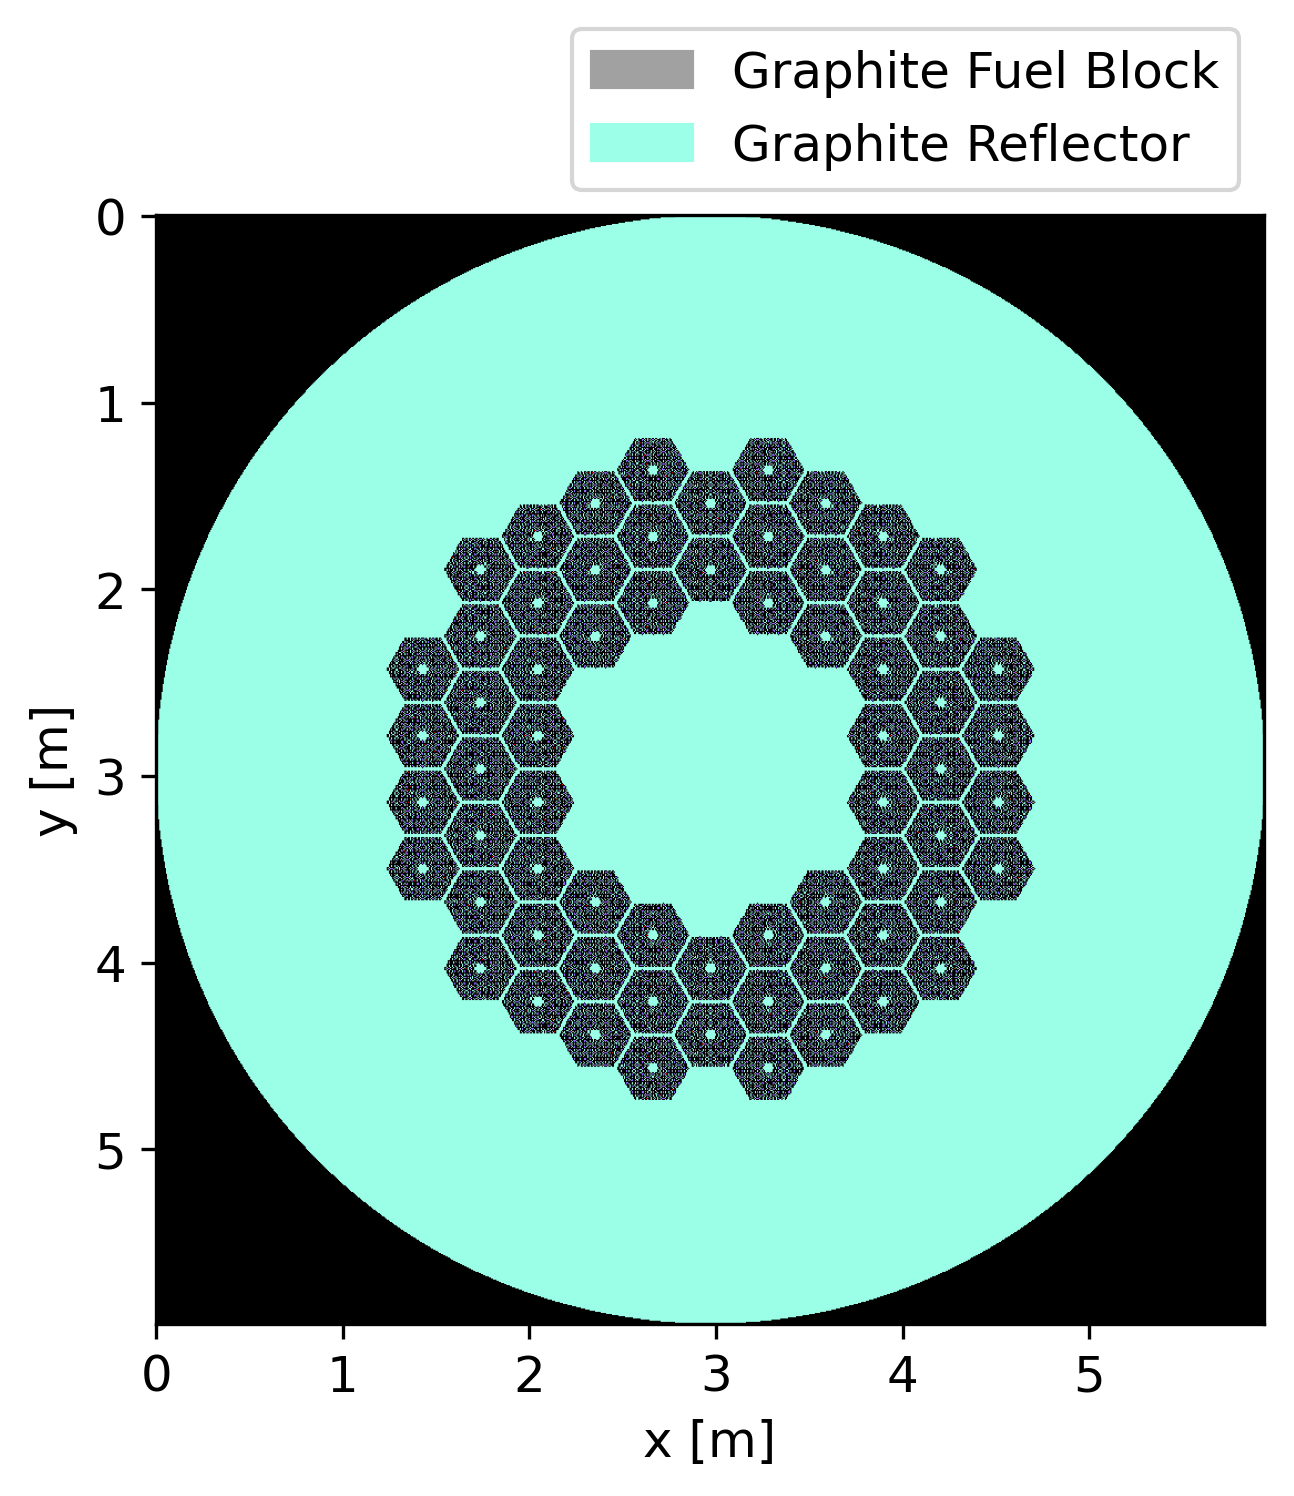
\includegraphics[width=0.39\textwidth]{figures-fullcore/oecd-fullcore}
    }
    \subfloat[Moltres model geometry.]{
        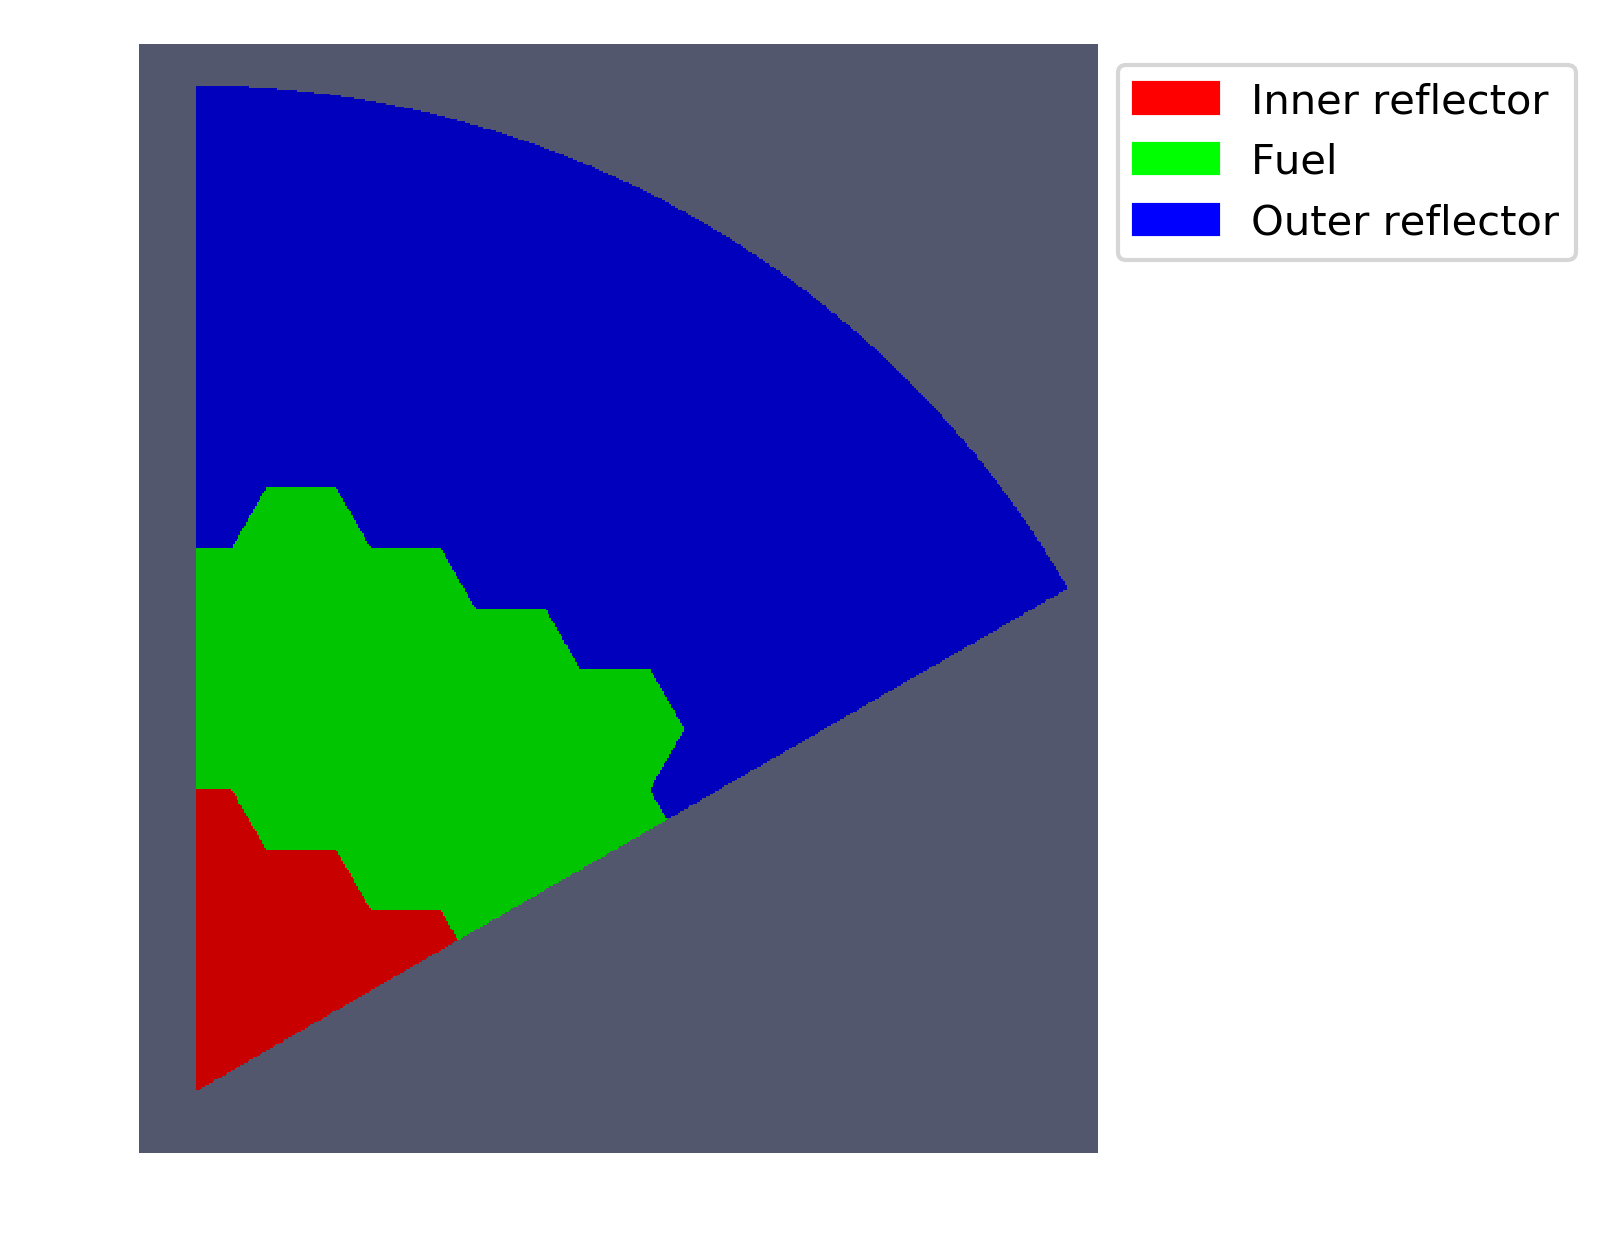
\includegraphics[width=0.49\textwidth]{figures-fullcore/3D-fullcore-60-homo-meshB2}
    }
	\hfill
  \caption{MHTGR-350 full-core models.}
	\label{fig:fullcoremodel}
\end{figure}

Taking advantage of the problem's symmetry, Moltres modeled only one-twelfth of the fuel column, Figure \ref{fig:fullcoremodel}.
We made the geometry and mesh using Gmsh.
The mesh had 300720 elements and 160035 nodes.
The diffusion calculations had 160035 \glspl{DoF}/energy-group and a total of 2400525 DoFs.
The Moltres input files set an eigenvalue and a flux convergence tolerance of 1$\times$10$^{-8}$.

% Keff
Between Serpent and Moltres, we compared the \gls{Keff}, the power distribution, and the flux shape and magnitude in different zones of the reactor.
Table \ref{tab:full-keff} exhibits the \gls{Keff} from Serpent and Moltres.
Moltres values are larger than Serpent's.
The values are within a 300 pcm difference.

\begin{table}[htbp!]
  \centering
  \caption{Serpent and Moltres eigenvalues.}
  \begin{tabular}{l|lll}
  \toprule
              & Serpent			& Moltres  & $\Delta \rho$ [pcm] 	\\
  \midrule
			 600K  	& 1.10869     & 1.11150	 &	228		\\
			1200K 	& 1.06138     & 1.06468	 &	292   \\

  \bottomrule
  \end{tabular}
  \label{tab:full-keff}
\end{table}

% Power distribution
Figures \ref{fig:fullcore-600-power} and \ref{fig:fullcore-1200-power} show Serpent and Moltres radial power distributions.
The following analysis applies to both temperatures.
The first thing that came to our attention is the symmetry of the power distribution.
The results are symmetric with respect to a 60$^{\circ}$ line.
This result suggests that we could reduce the mesh size by half by considering only one-twelfth of the reactor.
The next observation is that Moltres result exhibits a higher power density than Serpent in the inner and outer rings.
The power density in the middle ring is lower in the Moltres case.
The largest difference is in the inner ring.
Overall, the results differ in less than 0.30 MW.

%Power distribution at 600K
\begin{figure}[htbp!]
	\centering
    \subfloat[Moltres.]{
        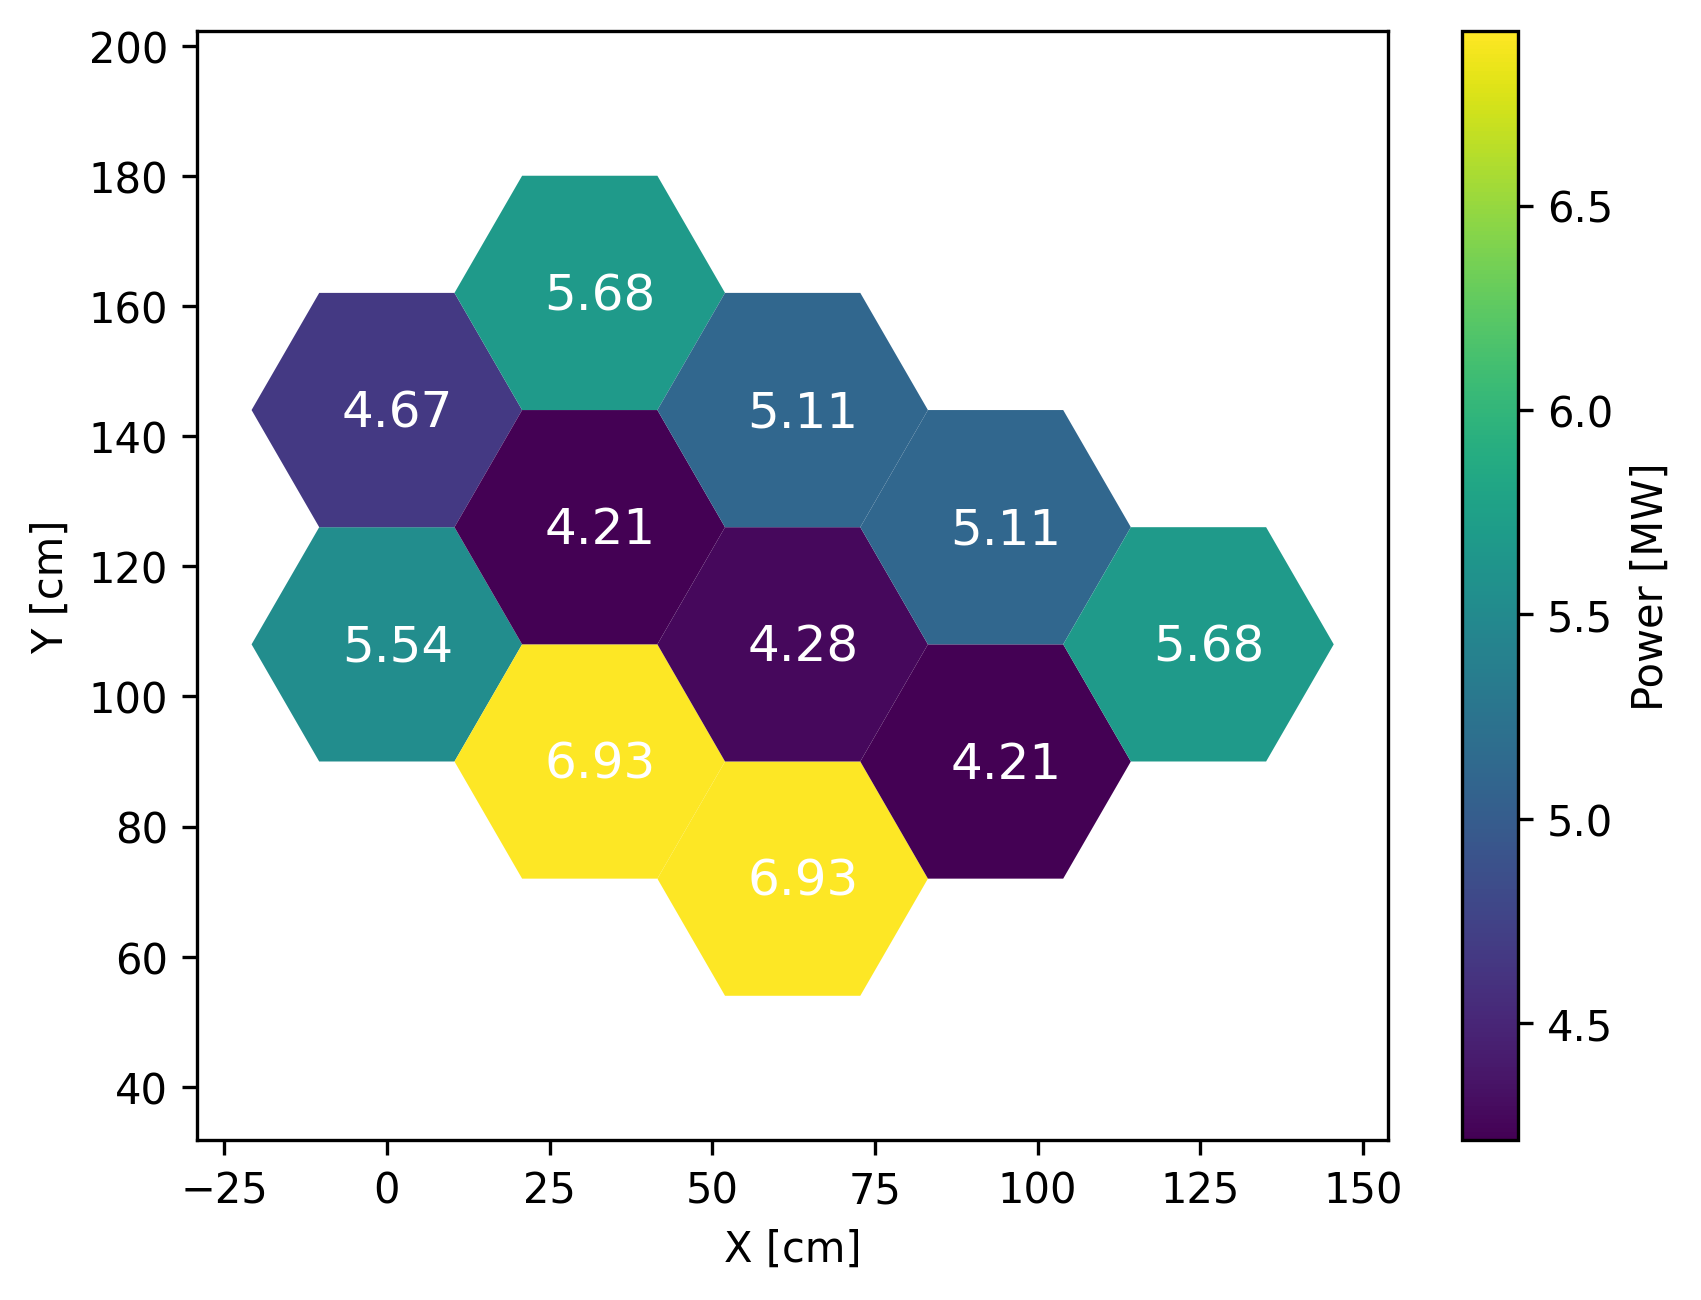
\includegraphics[width=0.45\textwidth]{figures-fullcore/3D-fullcore-600-15Gd-power}
    }
    \subfloat[Serpent.]{
        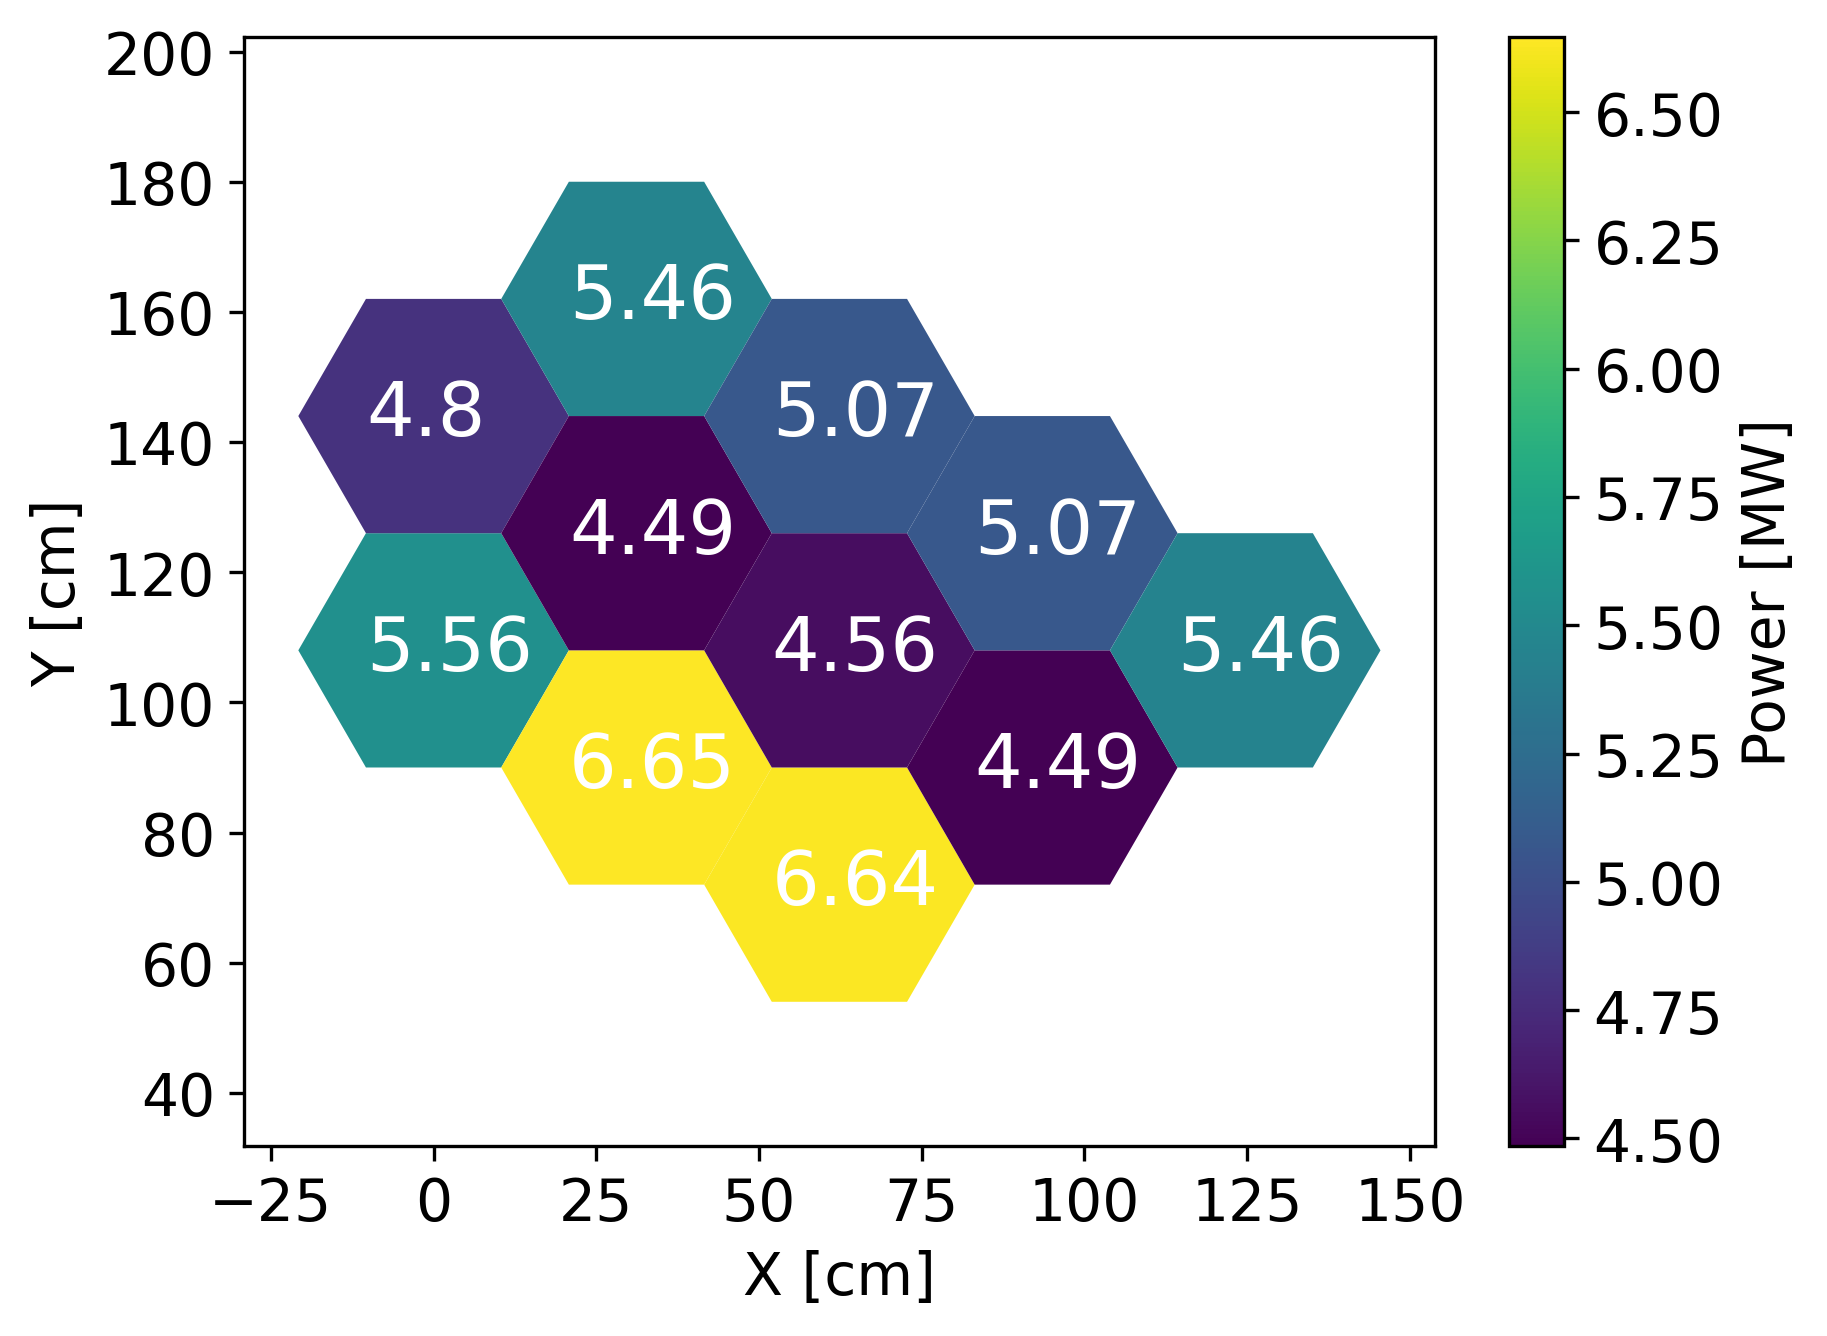
\includegraphics[width=0.45\textwidth]{figures-fullcore/serpent26G-600-power}
    }
	\hfill
	\caption{Radial power distribution at 600 K.}
	\label{fig:fullcore-600-power}
\end{figure}

%Power distribution at 1200K
\begin{figure}[htbp!]
	\centering
    \subfloat[Moltres.]{
        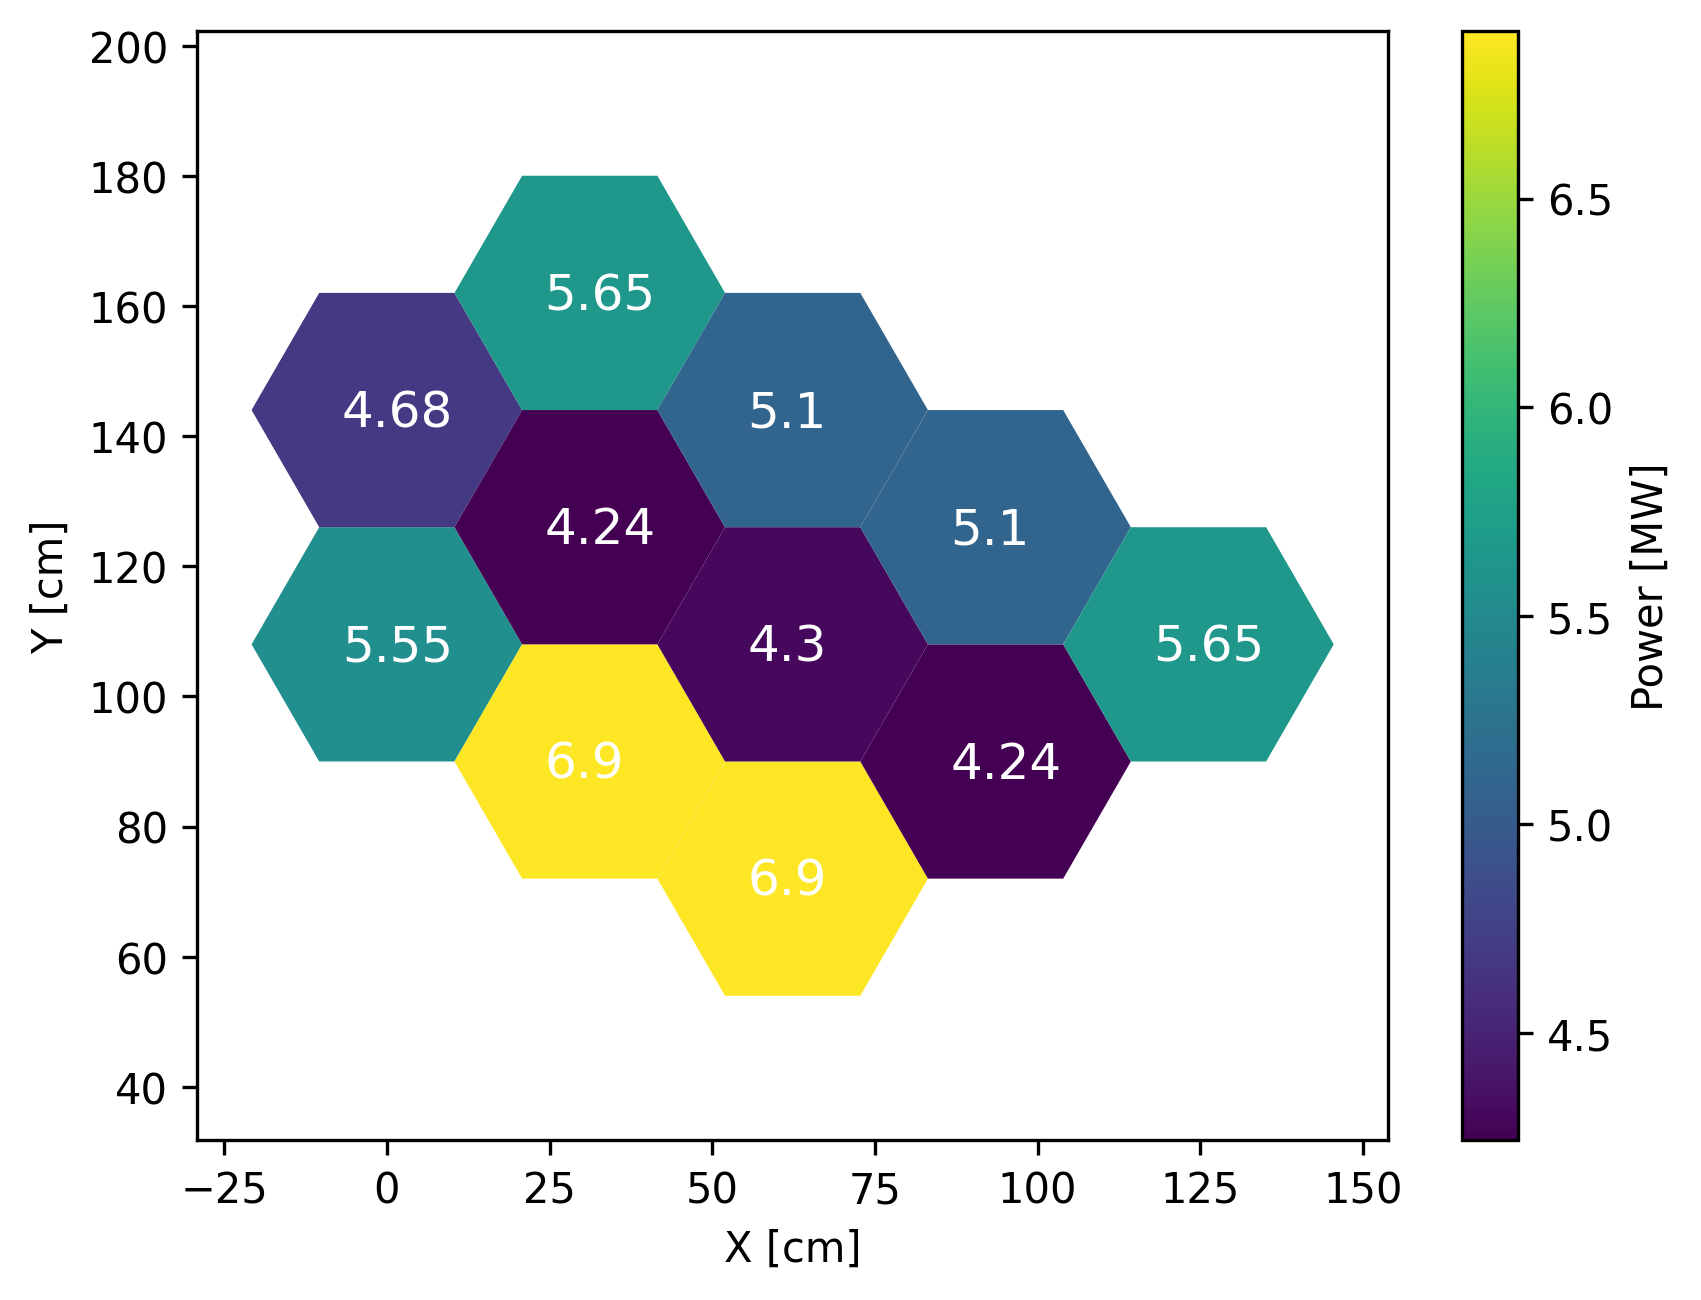
\includegraphics[width=0.45\textwidth]{figures-fullcore/3D-fullcore-1200-15Gc-power}
    }
    \subfloat[Serpent.]{
        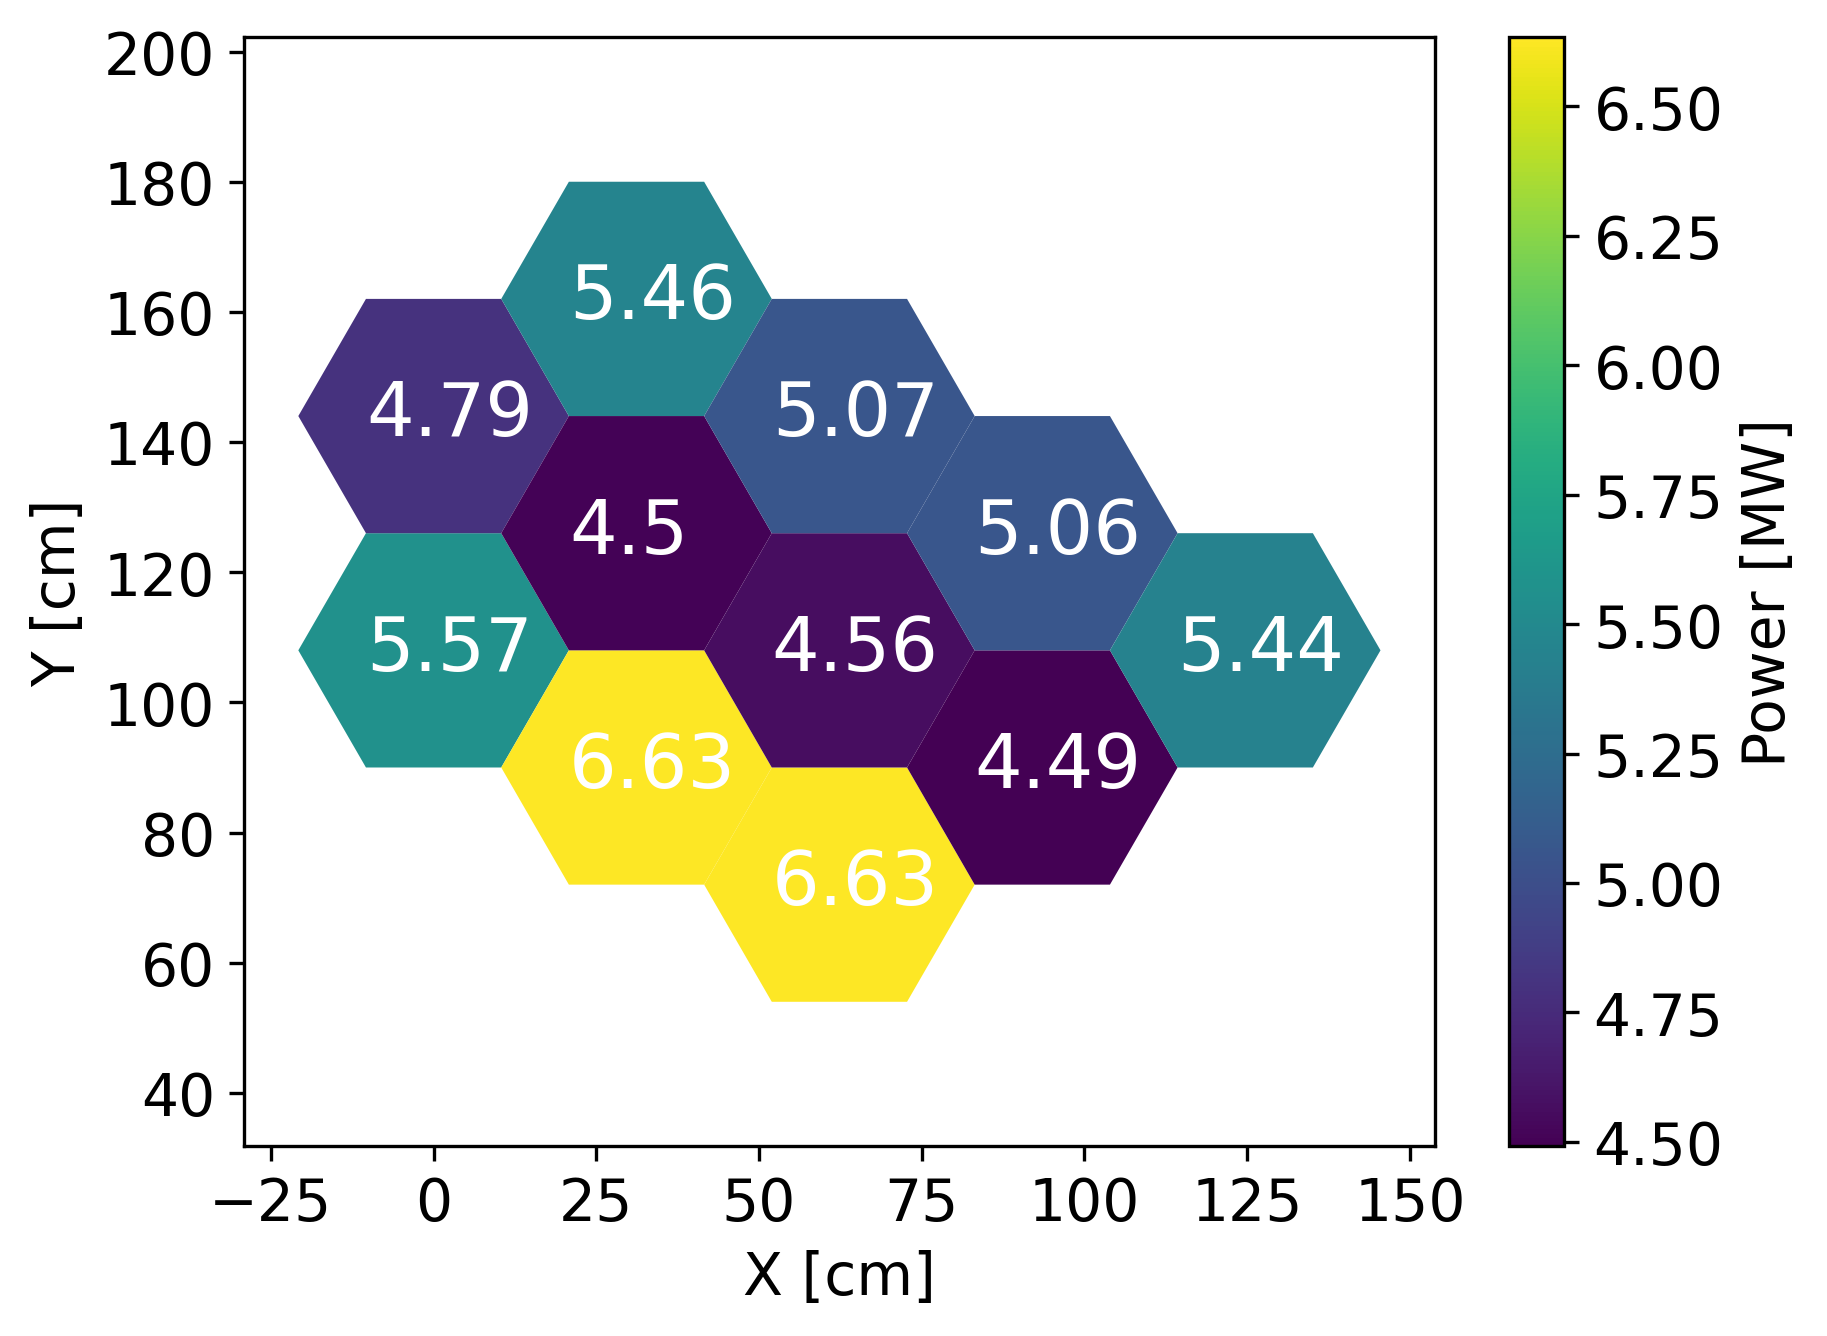
\includegraphics[width=0.45\textwidth]{figures-fullcore/serpent26G-1200-power}
    }
	\hfill
	\caption{Radial power distribution at 1200 K.}
	\label{fig:fullcore-1200-power}
\end{figure}

% Fluxes
We placed an axial and a radial flux detectors in arbitrary regions of the reactor to compare the fluxes.
Figure \ref{fig:fullcore-detectors} shows the location of the detectors.
Note that the flux in Serpent is an average over the fuel column's volume, while the flux in Moltres is the point-wise flux over the fuel column's centerline.
The Serpent radial detector's volume had a 2$^{\circ}$-angle and a fuel assembly's height.
Both the Serpent and Moltres radial detector's location was the middle of the active core's height.
Moltres ran the calculations for 15 energy groups and collapsed the results into three groups to facilitate the results' visualization.
Figures \ref{fig:fullcore-600-axial1} and \ref{fig:fullcore-600-radial1} show the axial and radial fluxes at 600K.
Figure \ref{fig:fullcore-600-axial1} shows that the fast and epithermal fluxes in Moltres are larger, while the thermal flux is smaller.
The flux shapes are similar.
The epithermal and thermal fluxes are closer in magnitude in the active core in Serpent's simulation.
In Figure \ref{fig:fullcore-600-radial1}, Serpent fluxes present some 'noise.'
A higher number of generations/cycle in Serpent simulations would solve it.
Another alternative is using a detector with a larger volume.
Additionally, the flux in Serpent shows the location of the LBPs in the fuel assemblies.
A diffusion solver fails to capture such localized effects as the group constants are homogeneous in the fuel assembly.
The fast flux in Moltres is larger, while the epithermal and thermal fluxes have almost the same magnitudes.
Figures \ref{fig:fullcore-1200-axial1} and \ref{fig:fullcore-1200-radial1} display the fluxes at 1200K.
These results differ from the 600K case.
However, we observe the same behavior for both axial and radial fluxes.

%Detectors
\begin{figure}[htbp!]
	\centering
    \subfloat[Moltres model.]{
        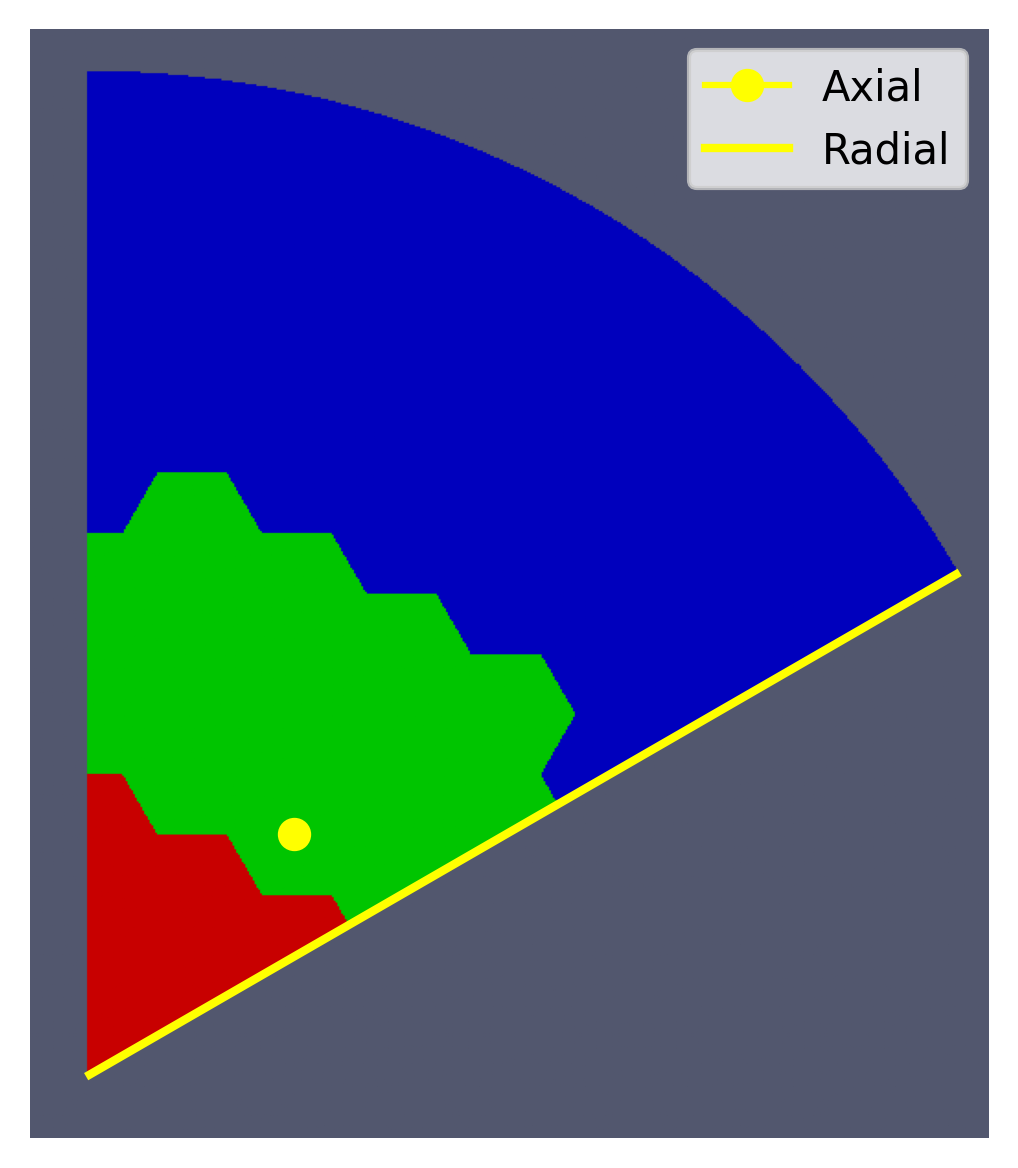
\includegraphics[width=0.37\textwidth]{figures-fullcore/3D-fullcore-60-detectors2}
    }
    \subfloat[Serpent model.]{
        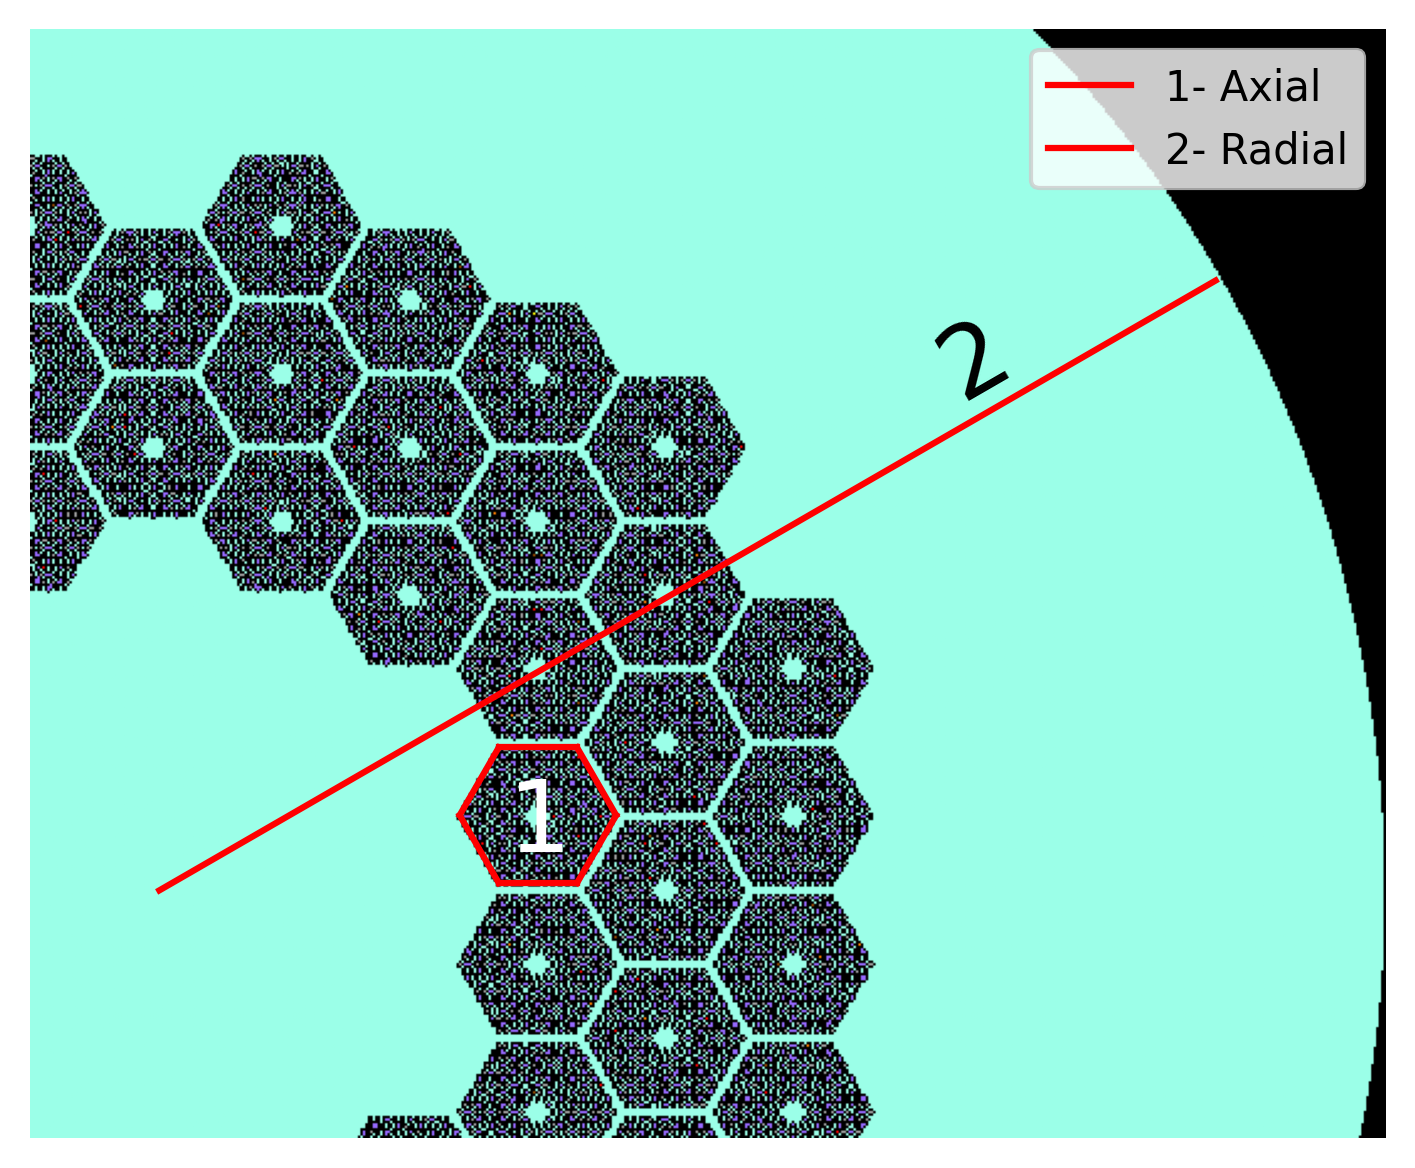
\includegraphics[width=0.52\textwidth]{figures-fullcore/oecd-fullcore-detectorsC}
    }
	\hfill
	\caption{Flux detector locations.}
	\label{fig:fullcore-detectors}
\end{figure}

% Axial flux1 at 600K
\begin{figure}[htbp!]
	\centering
    \subfloat[Moltres.]{
        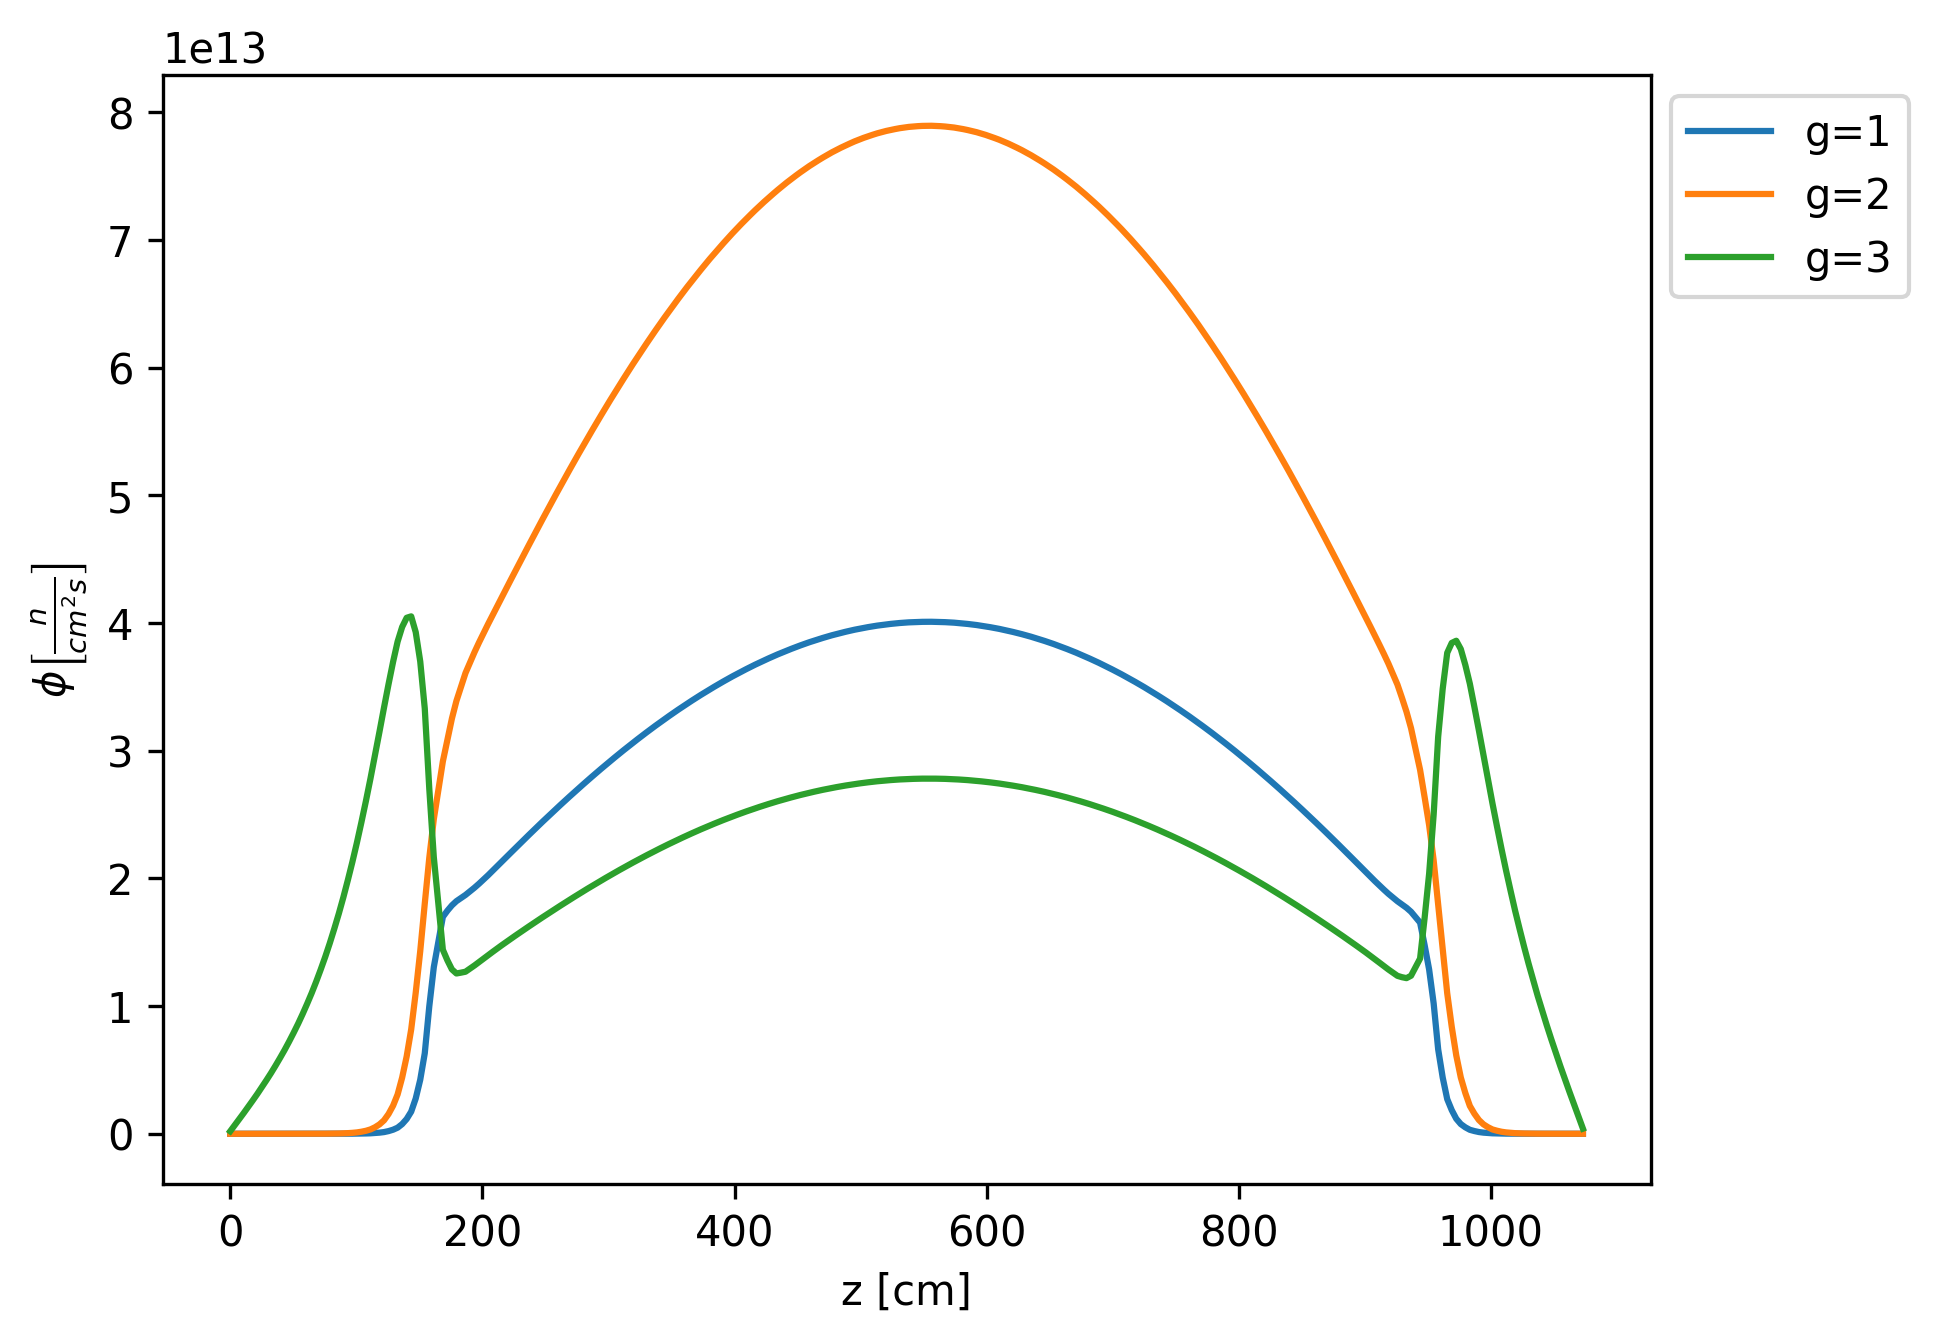
\includegraphics[width=0.45\textwidth]{figures-fullcore/3D-fullcore-600-15Gd-axial1}
    }
    \subfloat[Serpent.]{
        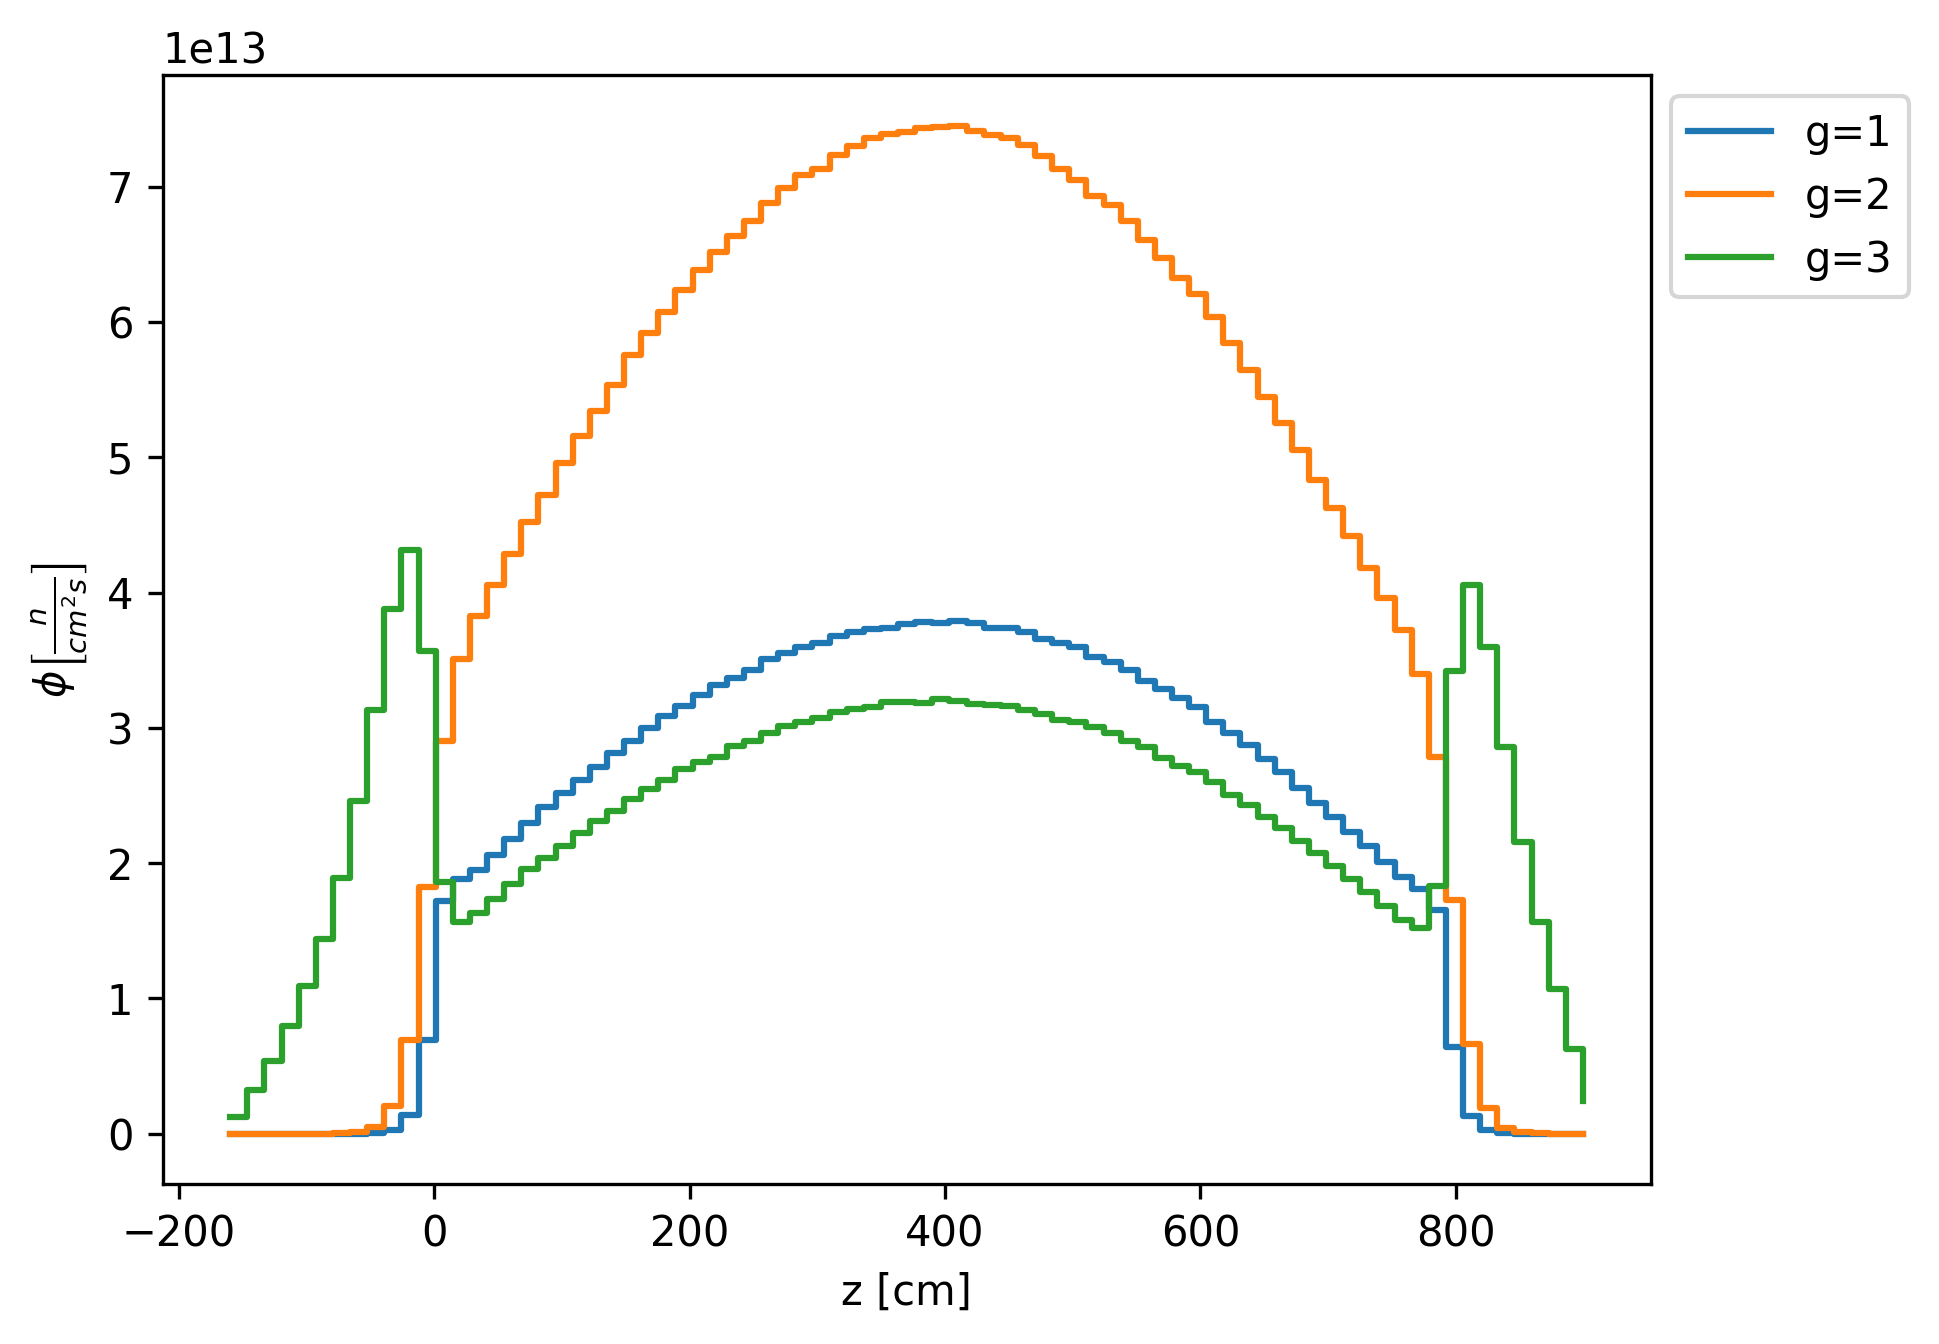
\includegraphics[width=0.45\textwidth]{figures-fullcore/serpent26G-600-collapse-Axial1}
    }
	\hfill
	\caption{Axial flux at 600 K.}
	\label{fig:fullcore-600-axial1}
\end{figure}

%Radial flux at 600 K
\begin{figure}[htbp!]
	\centering
    \subfloat[Moltres.]{
        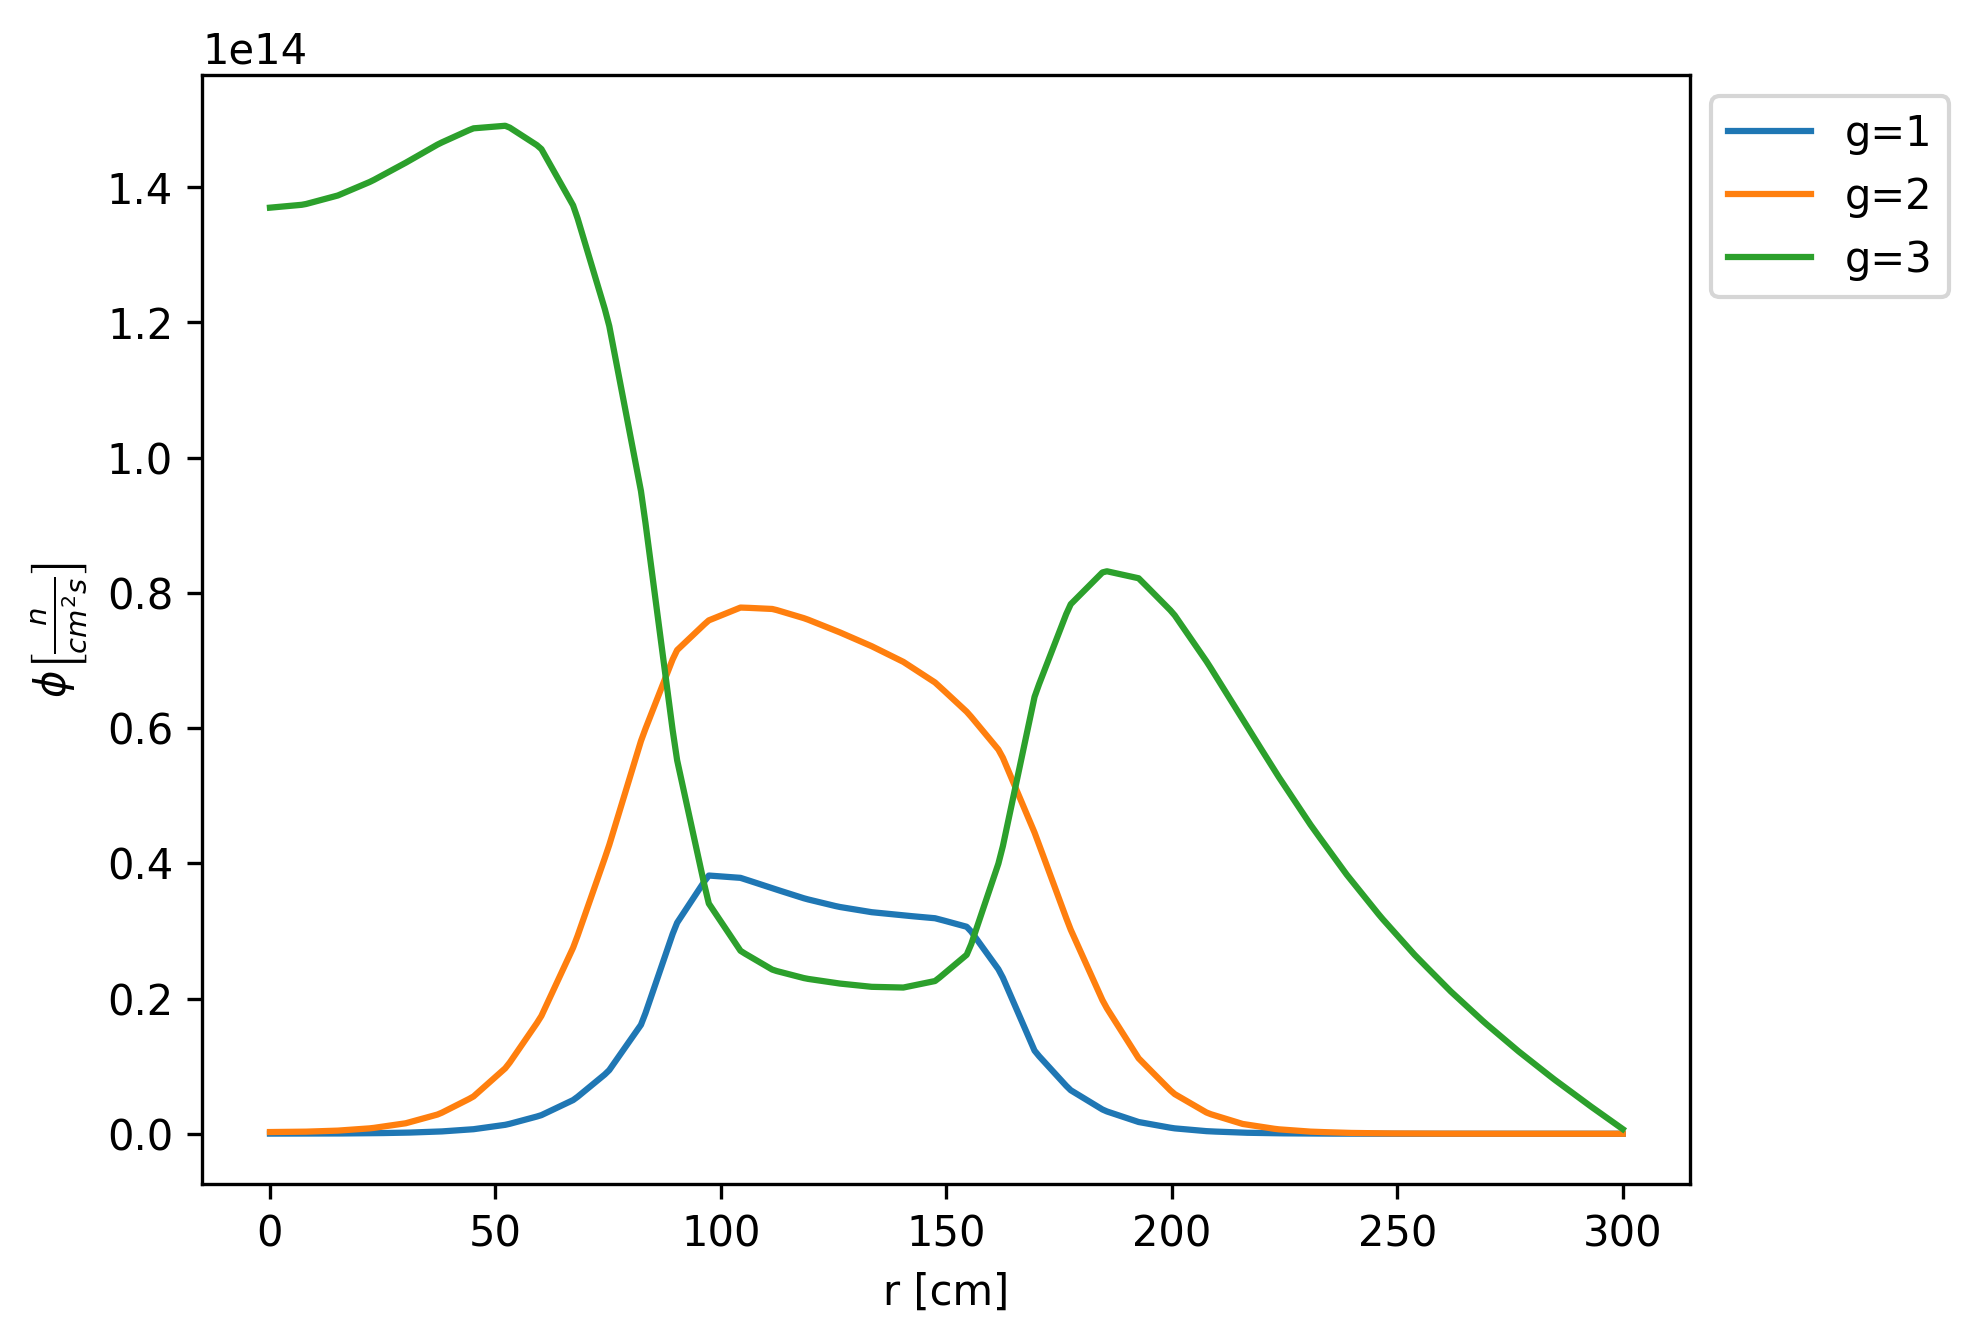
\includegraphics[width=0.45\textwidth]{figures-fullcore/3D-fullcore-600-15Gd-radial1}
    }
    \subfloat[Serpent.]{
        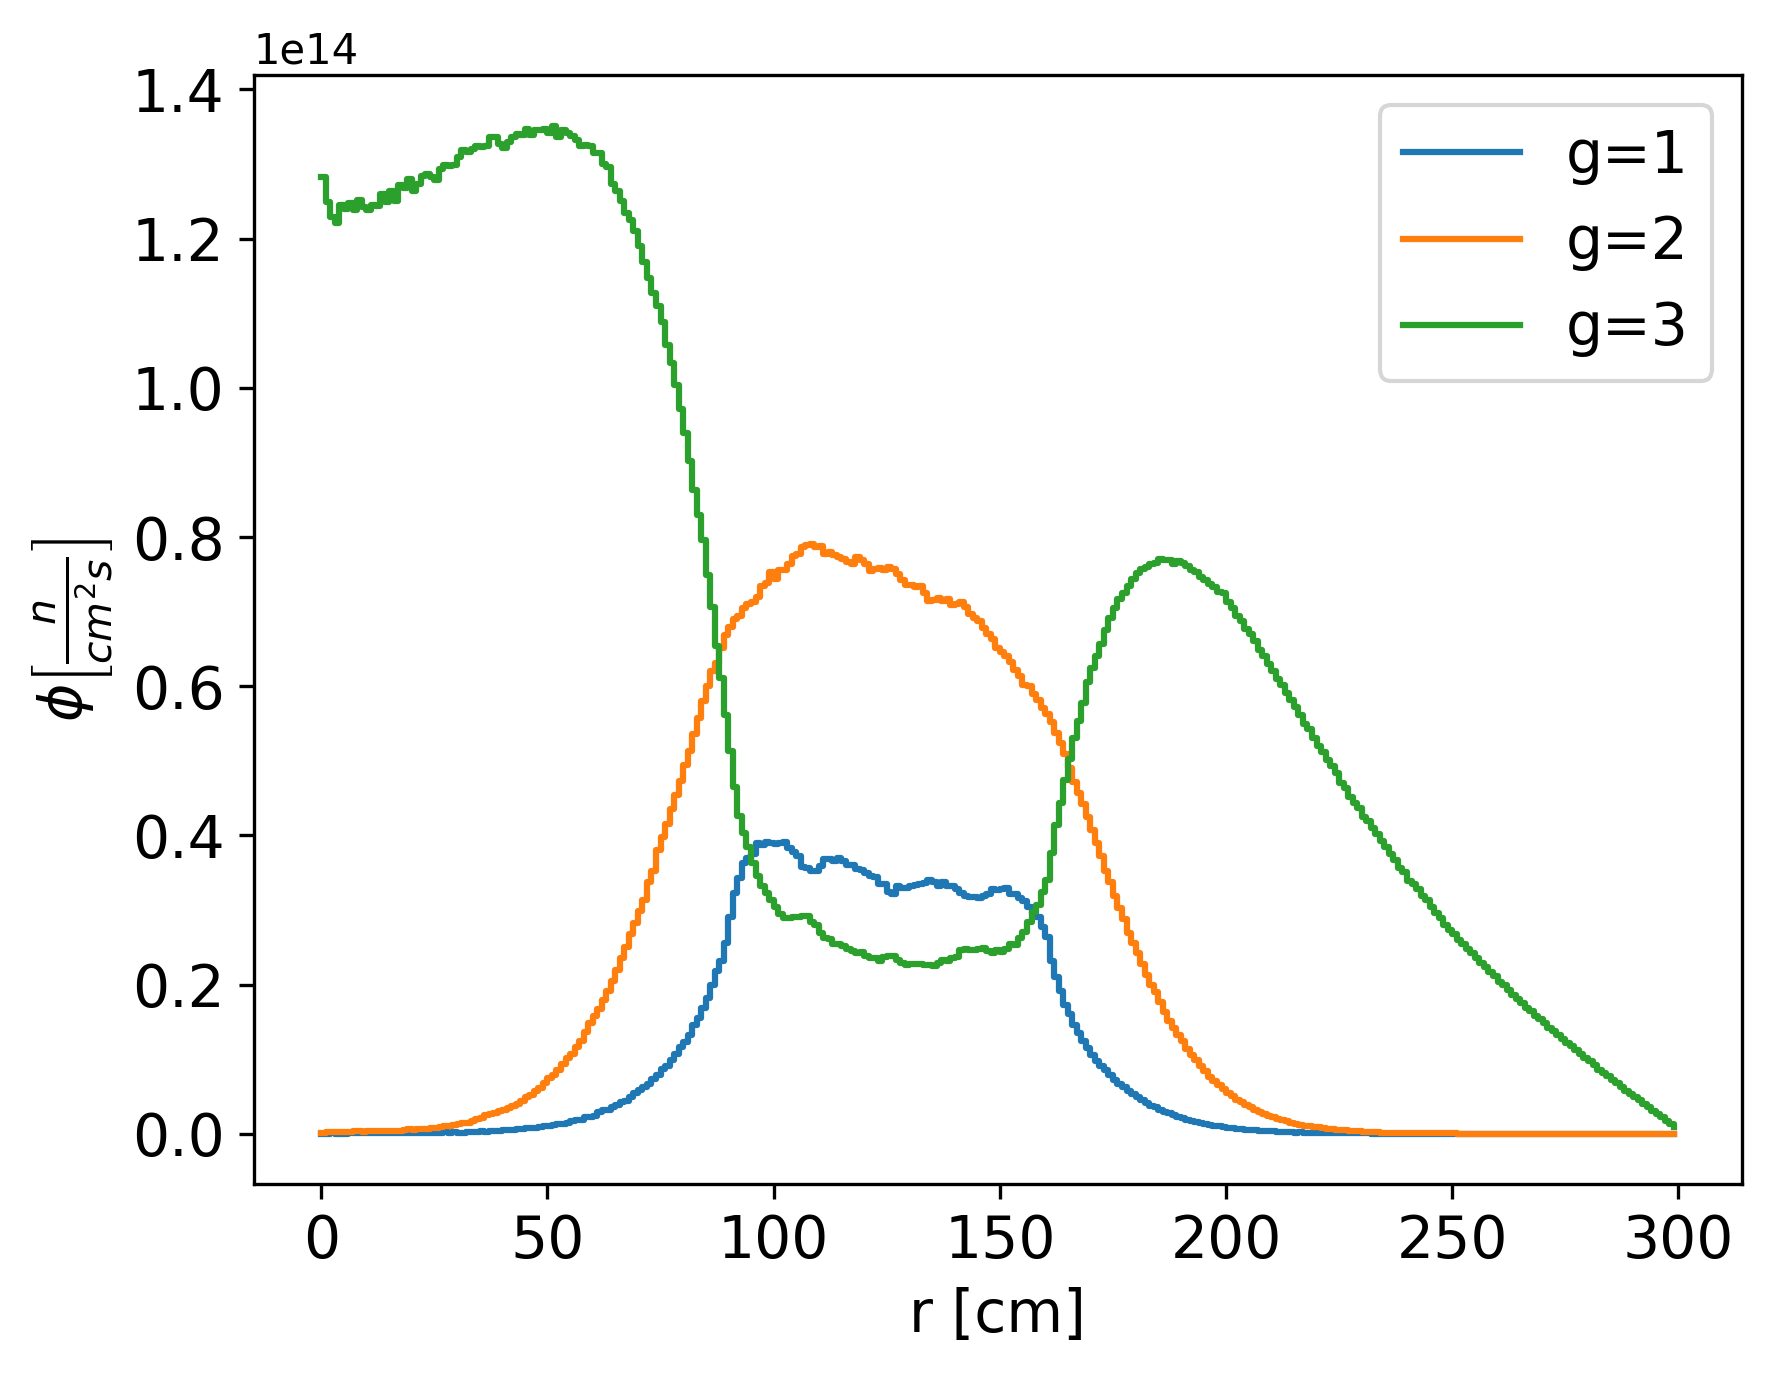
\includegraphics[width=0.45\textwidth]{figures-fullcore/serpent26G-600-collapse-Radial}
    }
	\hfill
	\caption{Radial flux at 600 K.}
	\label{fig:fullcore-600-radial1}
\end{figure}

% Axial flux1 at 1200K
\begin{figure}[htbp!]
	\centering
    \subfloat[Moltres.]{
        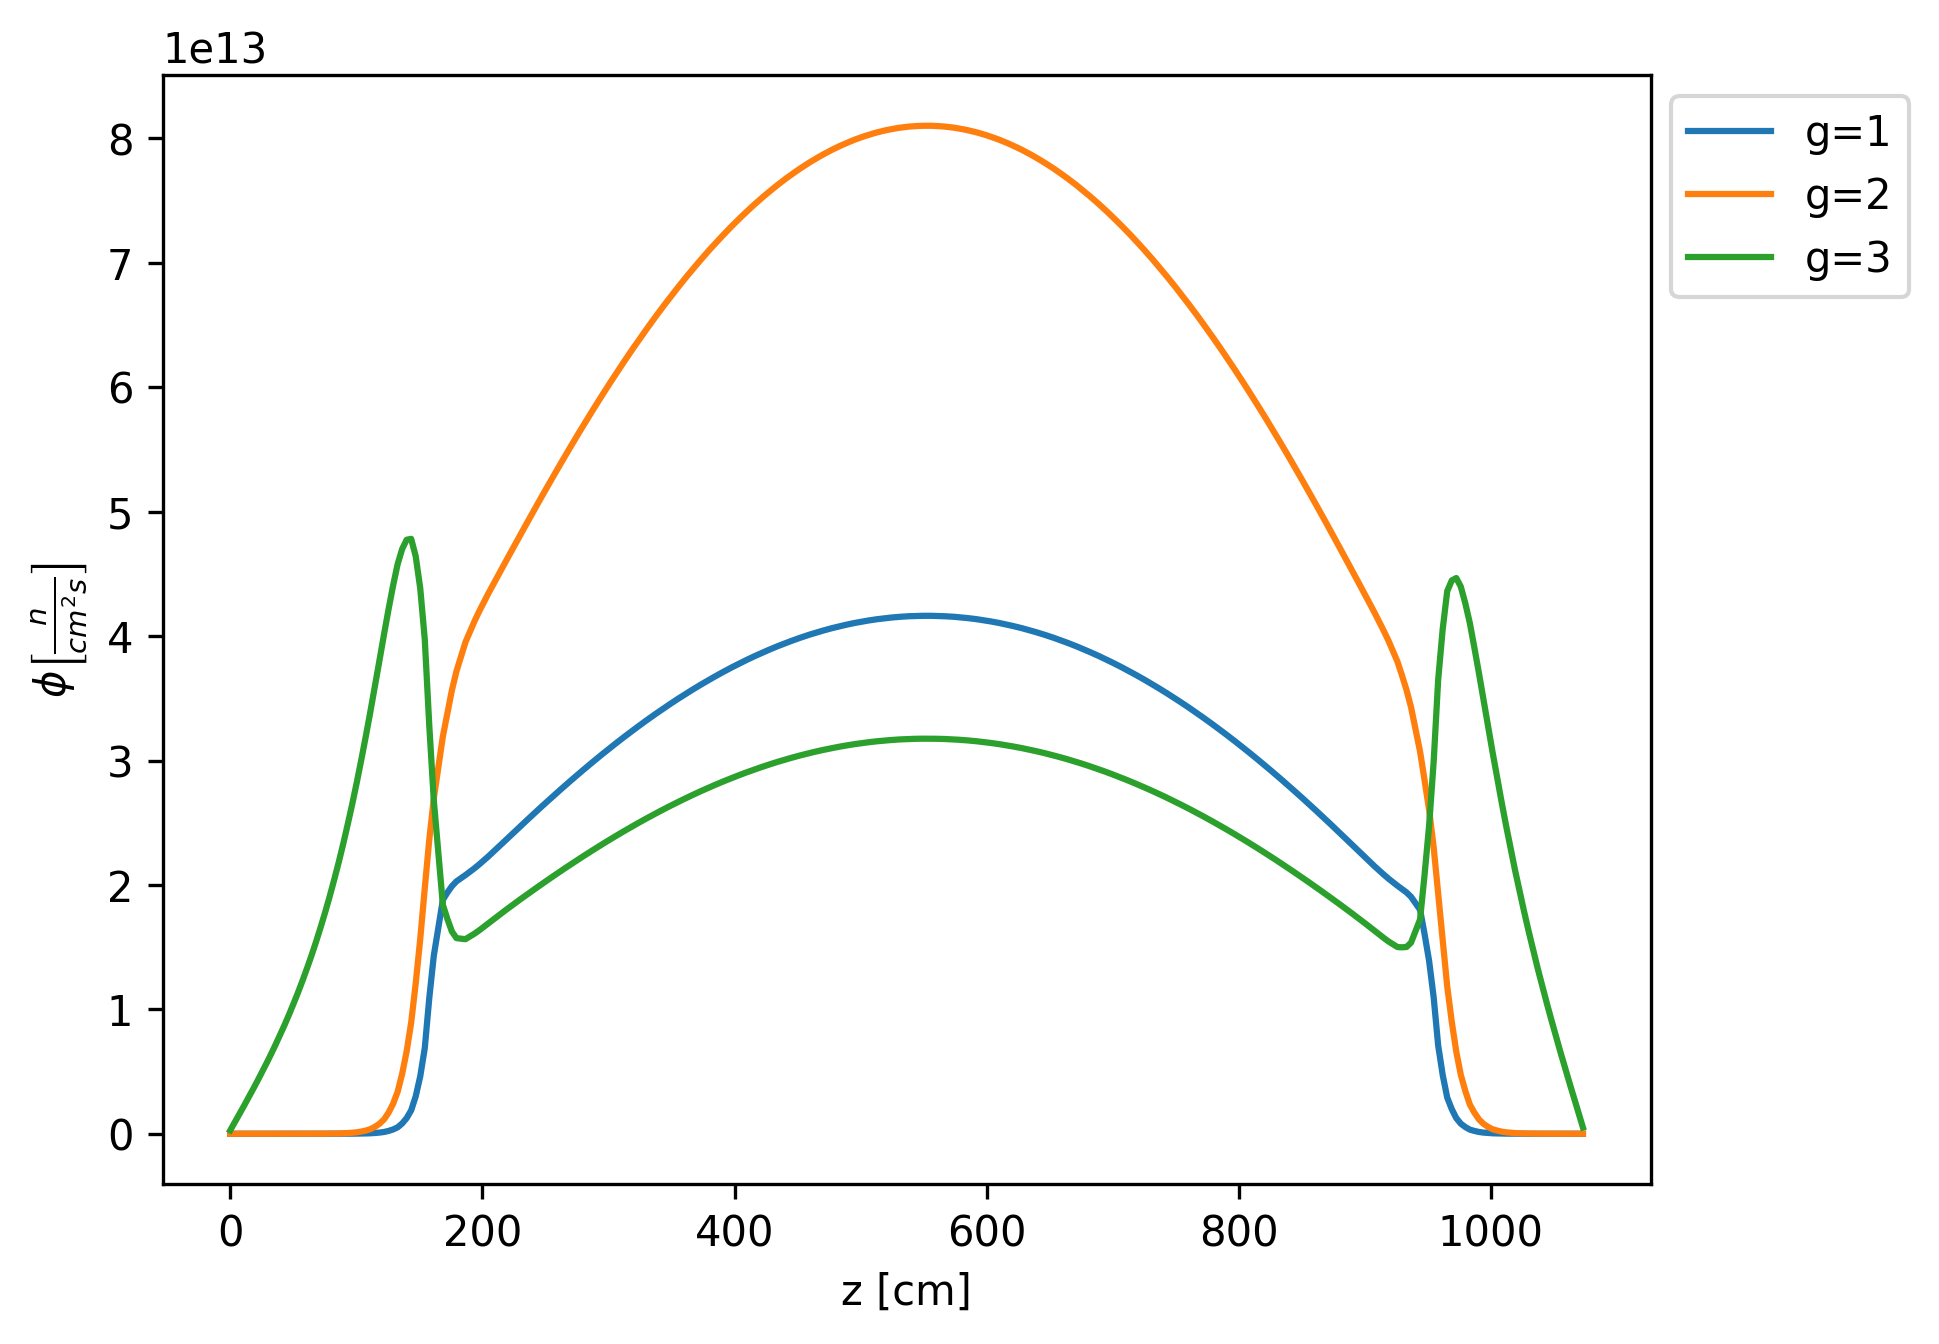
\includegraphics[width=0.45\textwidth]{figures-fullcore/3D-fullcore-1200-15Gc-axial1}
    }
    \subfloat[Serpent.]{
        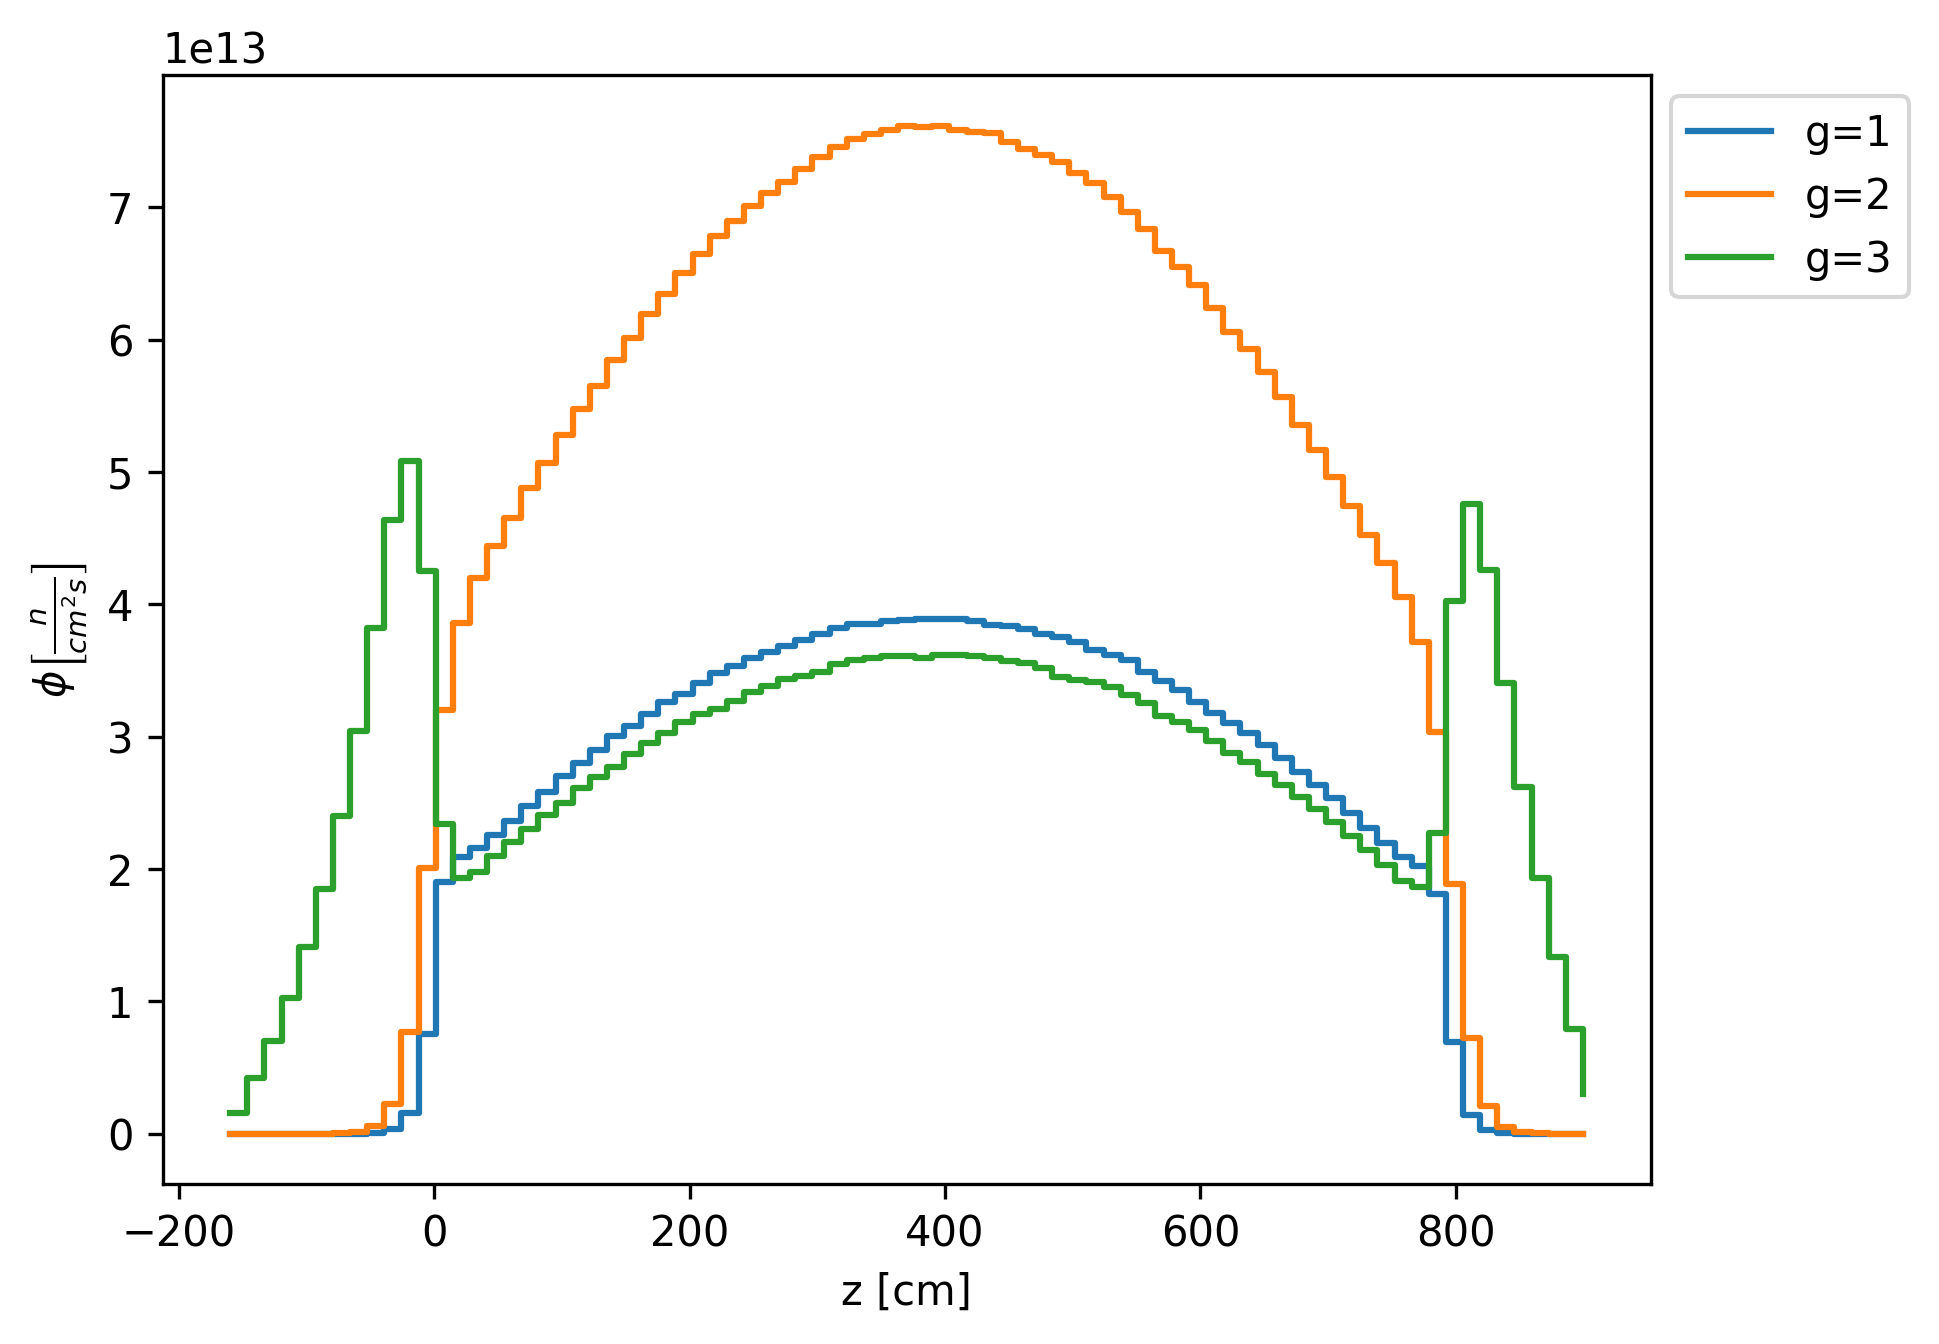
\includegraphics[width=0.45\textwidth]{figures-fullcore/serpent26G-1200-collapse-Axial1}
    }
	\hfill
	\caption{Axial flux at 1200 K.}
	\label{fig:fullcore-1200-axial1}
\end{figure}

%Radial flux at 1200 K
\begin{figure}[htbp!]
	\centering
    \subfloat[Moltres.]{
        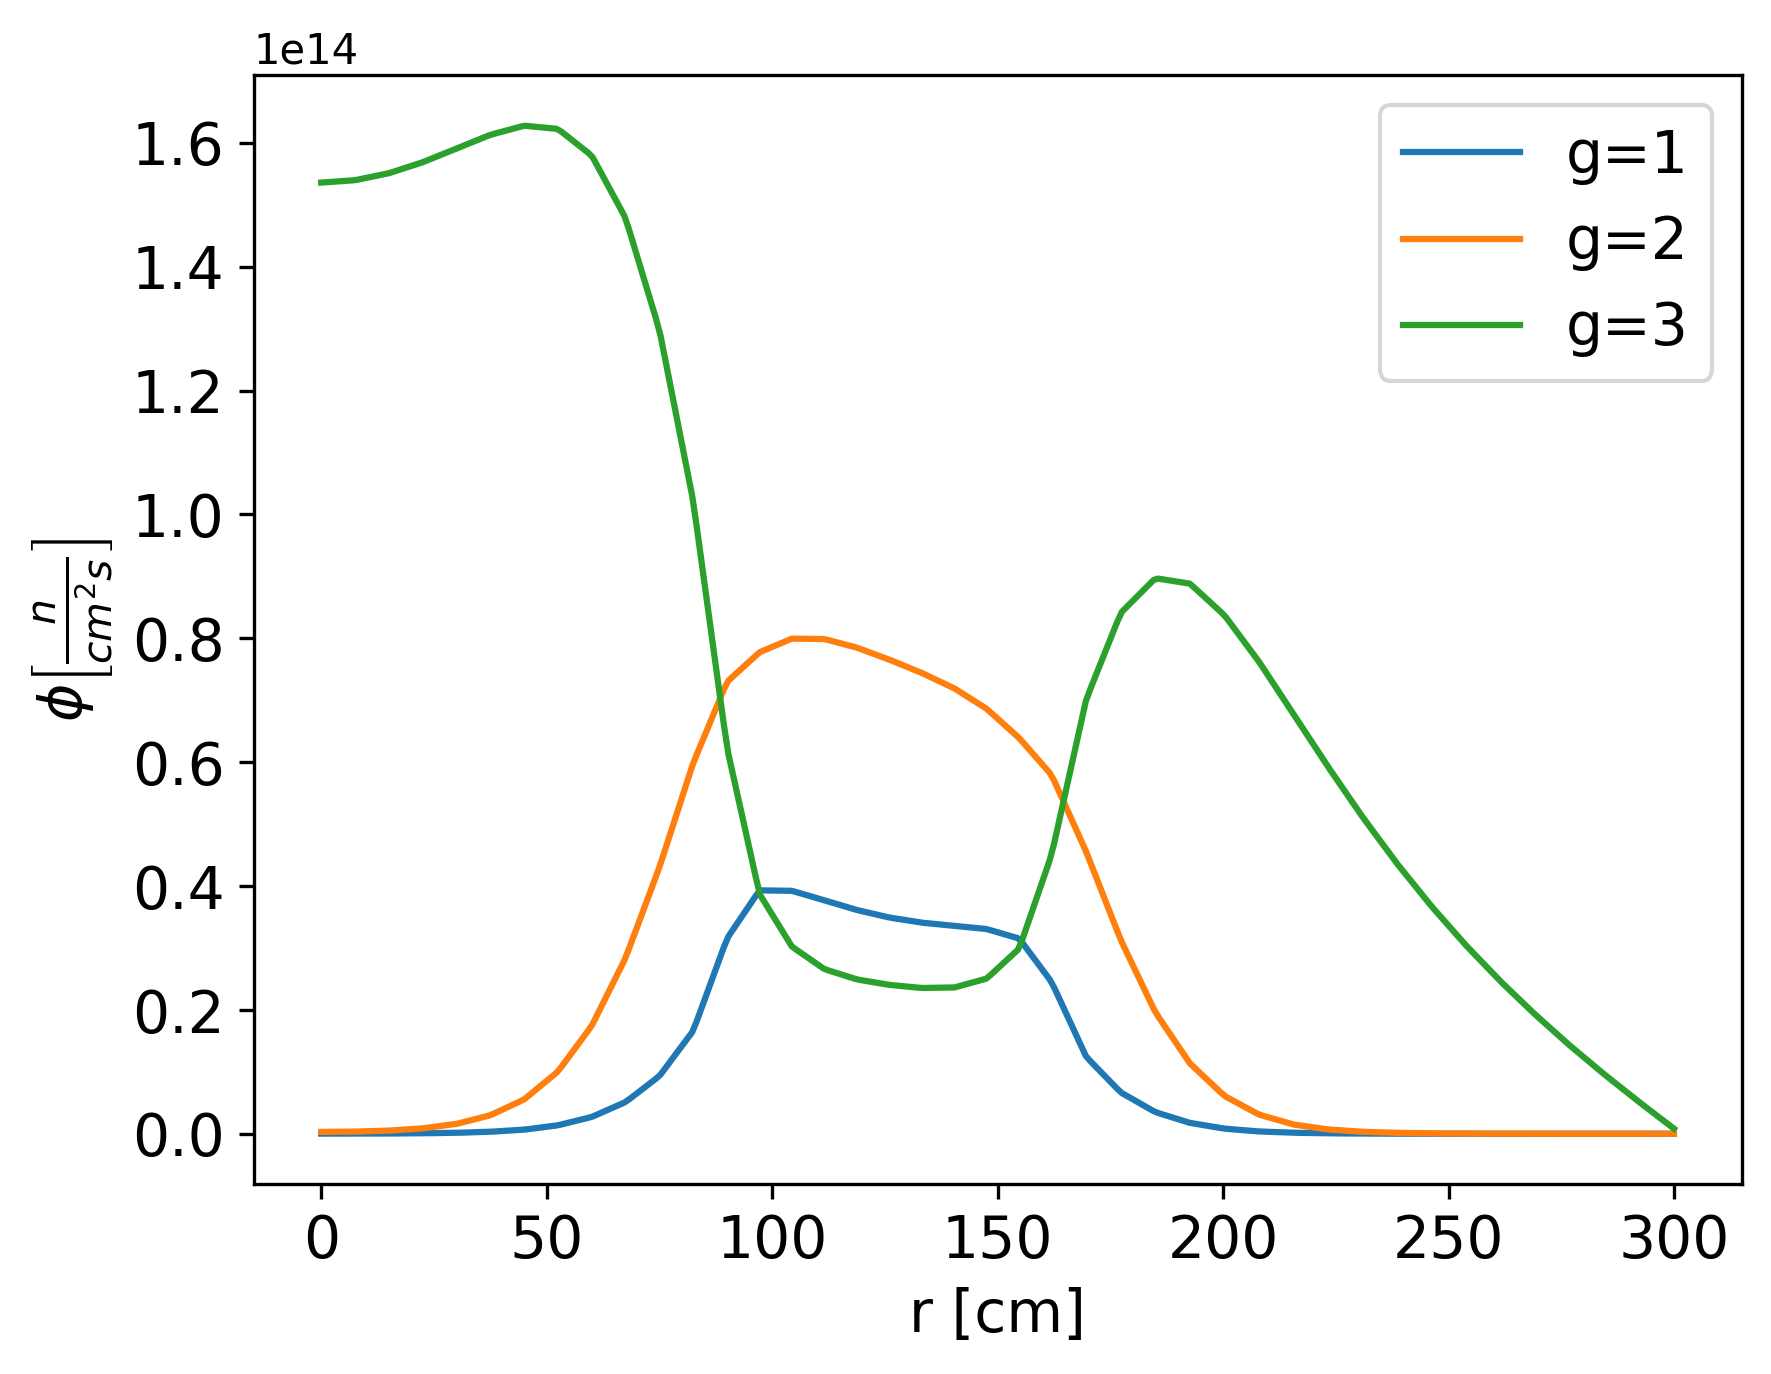
\includegraphics[width=0.45\textwidth]{figures-fullcore/3D-fullcore-1200-15Gc-radial1}
    }
    \subfloat[Serpent.]{
        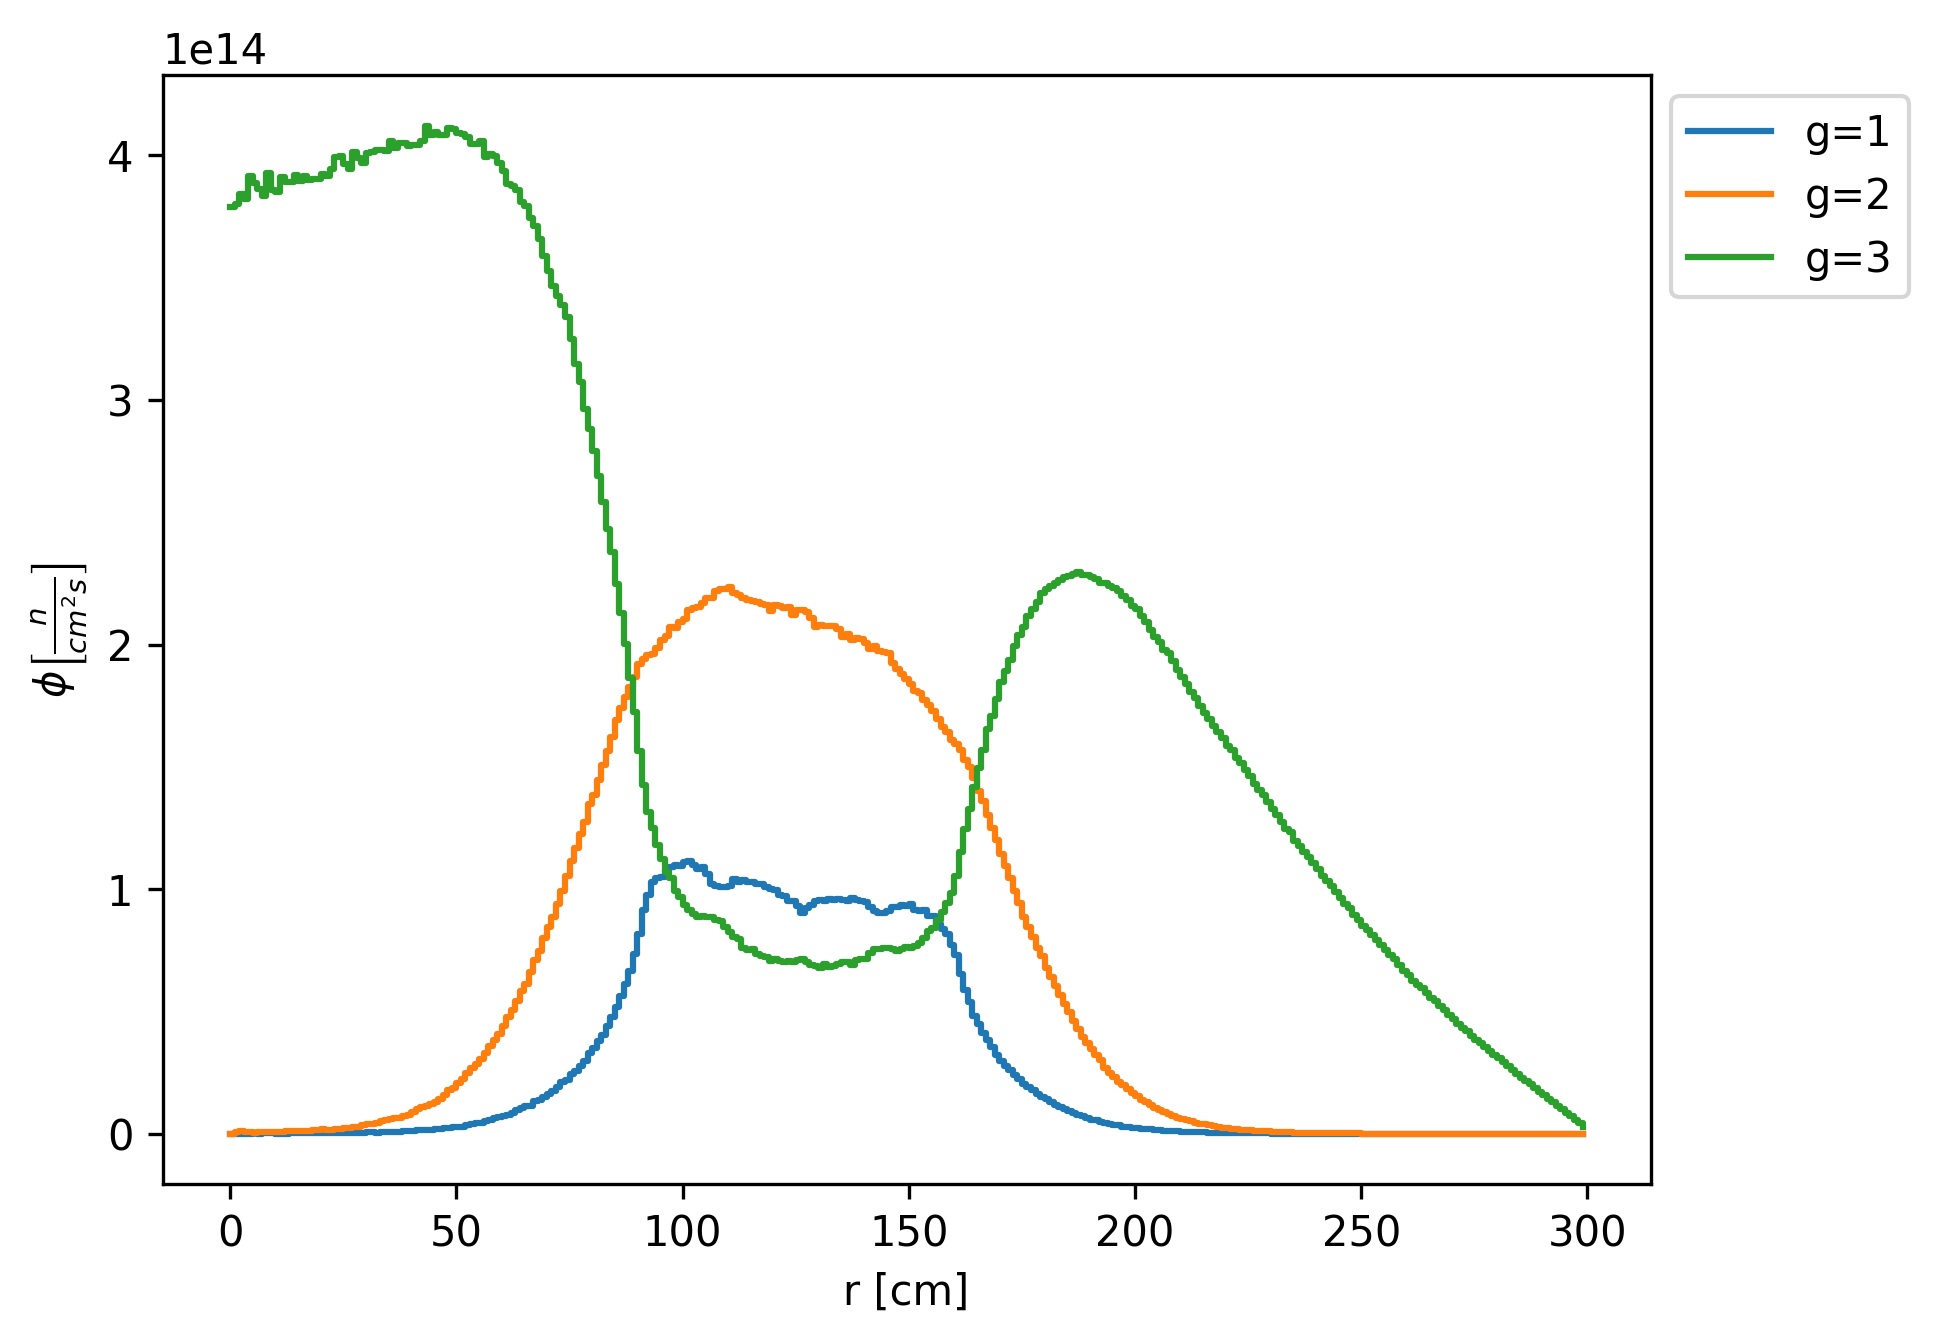
\includegraphics[width=0.45\textwidth]{figures-fullcore/serpent26G-1200-collapse-Radial}
    }
	\hfill
	\caption{Radial flux at 1200 K.}
	\label{fig:fullcore-1200-radial1}
\end{figure}


\section{OECD/NEA MHTGR-350 MW Benchmark: Phase I Exercise 1}

% Exercise description
This section conducted Phase I Exercise 1 of the benchmark with Moltres and compared the results with the already published results \cite{oecd_nea_coupled_2020}.
The benchmark specifies the group constants required to conduct the exercise.
The group constants provision ensures a common dataset among various benchmark participants and allows for comparing stand-alone neutronic predictions with no thermal-fluids feedback.
% What should be reported \cite{oecd_nea_benchmark_2017}
The exercise requests the reporting of the global parameters: $K_{eff}$, \gls{CR} worth ($\Delta \rho_{CR}$), and axial offset ($AO$).
% It also requires the reporting of a power distribution and a neutron-flux map \cite{oecd_nea_benchmark_2017}.
It also requires the reporting of a power distribution map \cite{oecd_nea_benchmark_2017}.
Equations \ref{eq:controlrod} and \ref{eq:ao} define $\Delta \rho_{CR}$ and $AO$.
\begin{align}
    \Delta \rho_{CR} &= \frac{k_{out}-k_{in}}{k_{out}k_{in}}
		\label{eq:controlrod}
    \intertext{where}
    k_{out} &= \mbox{eigenvalue with \gls{CR} out (at position 1184.8 cm)} \notag \\
    k_{in} &= \mbox{eigenvalue with \gls{CR} in (at position 391.81 cm)} \notag
		\intertext{and}
    AO &= (TP_{top}-TP_{bottom})/(TP_{top}+TP_{bottom})
		\label{eq:ao}
    \intertext{where}
    TP_{top} &= \mbox{total power produced in the top half core} \notag \\
    TP_{bottom} &= \mbox{total power produced in the bottom half core.} \notag
\end{align}

Moltres modeled one-third of the reactor, Figure \ref{fig:bench-mesh}.
The model included the bottom and top reflectors.
The core comprised 232 hexagonal subdomains for which the benchmark provides their group constants.
Table \ref{tab:mac-region} lists the six macroscopic regions that we can differentiate in the model.
The simulations required two meshes: one for the CR out and one for the CR in.
The simulation with the CR out had 268393 \glspl{DoF}/energy-group, and a total of 6978218 DoFs.
The simulation with the CR in had 227592 \glspl{DoF}/energy-group, and a total of 5917392 DoFs.
The Moltres input files set an eigenvalue convergence tolerance of 1$\times$10$^{-8}$.

\begin{figure}[htbp!]
	\centering
	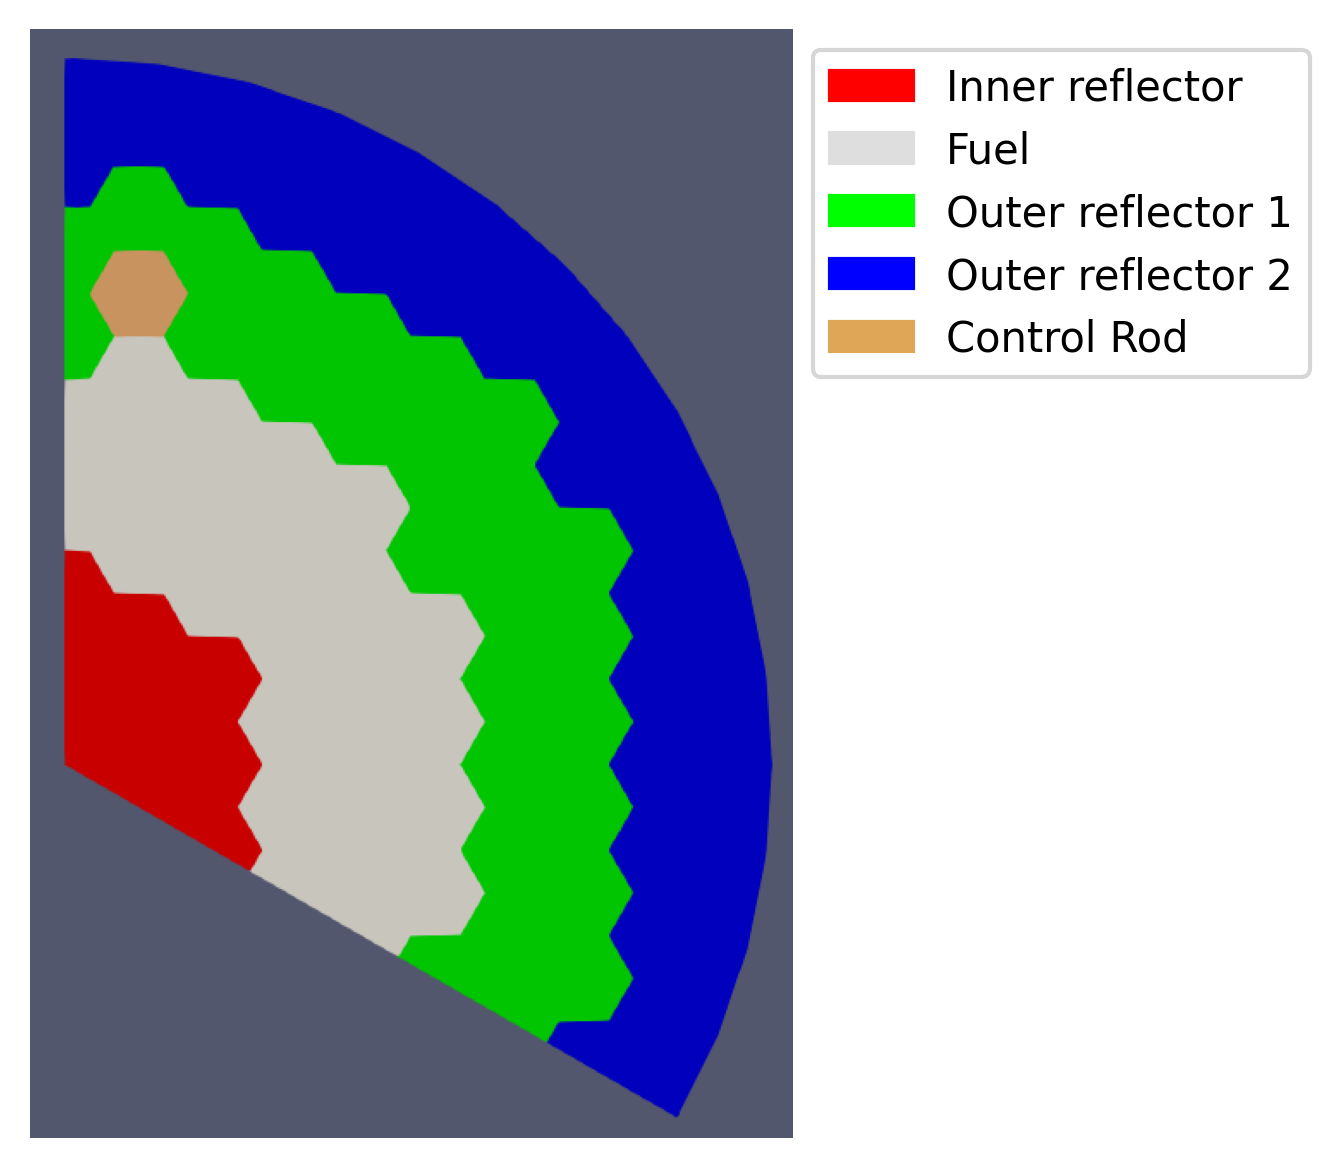
\includegraphics[width=0.55\linewidth]{figures-benchmark/oecd-fullcore-legend}
	\hfill
	\caption{1/3$^{rd}$ of the MHTGR-350 geometry.}
	\label{fig:bench-mesh}
\end{figure}

\begin{table}[htbp!]
  \centering
  \caption{Macroscopic regions.}
  \label{tab:mac-region}
  \begin{tabular}{@{}l c}
  \toprule
  Macroscopic region    & Subdomains     \\
  \midrule
  Fuel              & 1 to 220      \\
  Bottom reflector  & 221 to 224    \\
  Inner reflector   & 225           \\
  Outer reflector   & 226-227       \\
  Top reflector     & 228 to 231    \\
  Control Rod       & 232           \\
  \bottomrule
  \end{tabular}
\end{table}

The benchmark exercise specifies the group constants and the group constants numbering map.
The benchmark definition used DRAGON-4 \cite{marleau_user_2016} to obtain the group constants from a full block configuration.
The dataset contains 26 energy groups.
Among the benchmark group constants, we find $\Sigma_g^t$, $D_g$, $\nu\Sigma_g^f$, $\Sigma_g^f$, $\chi_g^t$, and $\Sigma_{g'\rightarrow g}^s$ (see equation \ref{eq:diffusion}).
The benchmark group constants format differs from Moltres'.
Hence, we made a python script to handle the formatting differences.

The benchmark exercise sets periodic \glspl{BC} on the sides of the geometry.
However, a memory issue did not allow for implementing those BCs in our 26-group Moltres input file.
We approximated the periodic BC with the reflective BC.
Section \ref{sec:bench-bcs} discusses further the use of periodic and reflective BCs.

% 4.33 h and 4.11 h
On average, the simulations took 4.22 hours using 1024 cores.
Table \ref{tab:globalparam} shows the main results.
Moltres predicted a \gls{Keff} larger than the reference result.
The reactivity difference is of 99 pcm.
Moltres yields a smaller control rod worth.
The difference is of 312 pcm.
The axial offset for the Moltres simulation is 4$\%$ higher than the reference result.
We attribute the discrepancies to the use of the reflective BCs instead of the periodic BCs.
Once again, Section \ref{sec:bench-bcs} discusses further the use of periodic and reflective BCs.

\begin{table}[htbp!]
  \centering
  \caption{Global parameters.}
  \begin{tabular}{l|l|l}
  \toprule
  Parameter 	&  Benchmark  &  Moltres    \\
  \midrule
  K$_{eff}$ 	&  1.06691    &  1.06804    \\
  $\Delta \rho_{CR}$ [pcm]  & 822.1 	& 509.8 \\
  AO        	&  0.168      &  0.1753     \\
  \bottomrule
  \end{tabular}
  \label{tab:globalparam}
\end{table}

Figure \ref{fig:axialpower} shows the radially averaged axial power distribution.
Moltres' result is close in shape and magnitude to the reference result.
Figure \ref{fig:radialpower} shows the axially averaged radial power distribution.
Moltres' values are similar to the reference results.
Moltres' power distribution in the inner ring is larger.
The differences are within 0.25 W/cm$^3$.


\begin{figure}[htbp!]
	\centering
    \subfloat[Moltres result.]{
        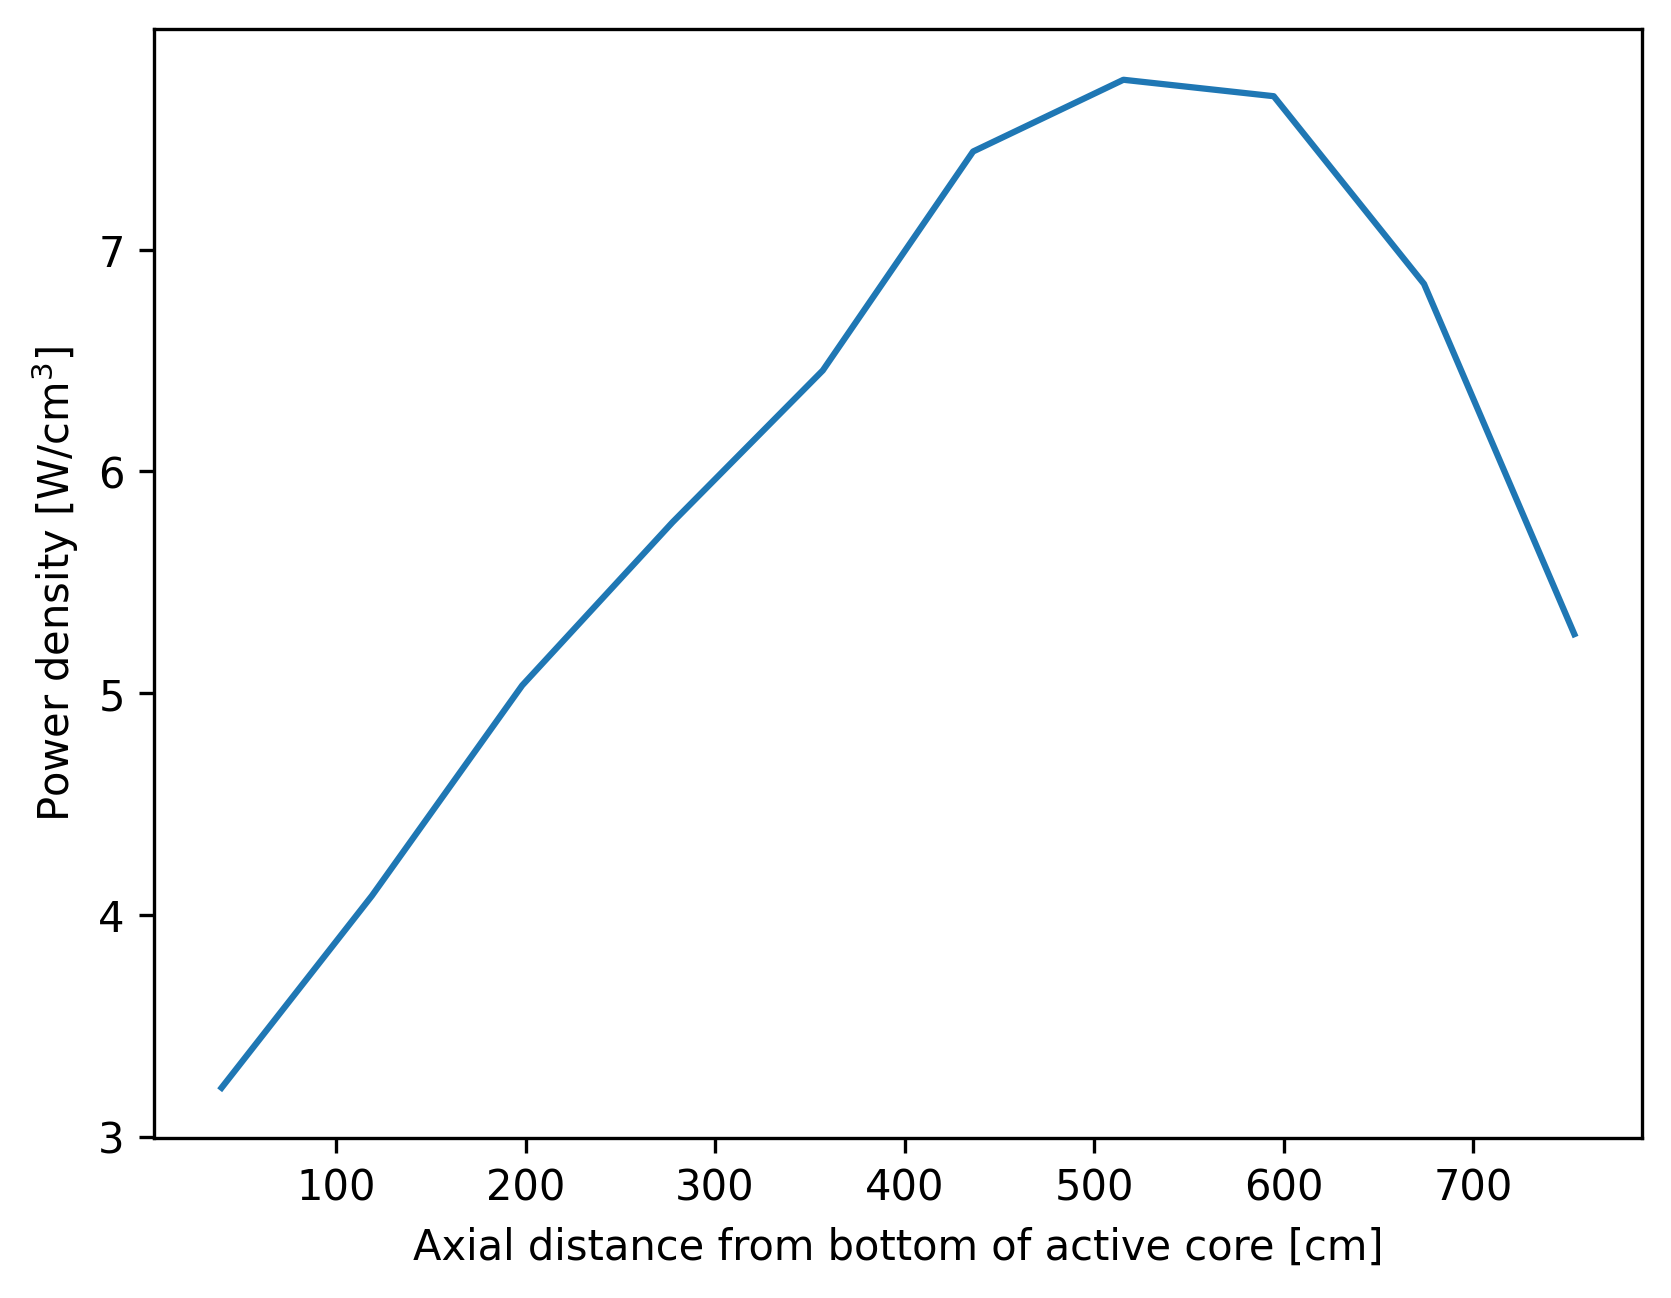
\includegraphics[width=0.42\textwidth]{figures-benchmark/3D-fullcore26G-axialpower}
    }
    \subfloat[Benchmark result. Image reproduced from \cite{oecd_nea_coupled_2020}.]{
        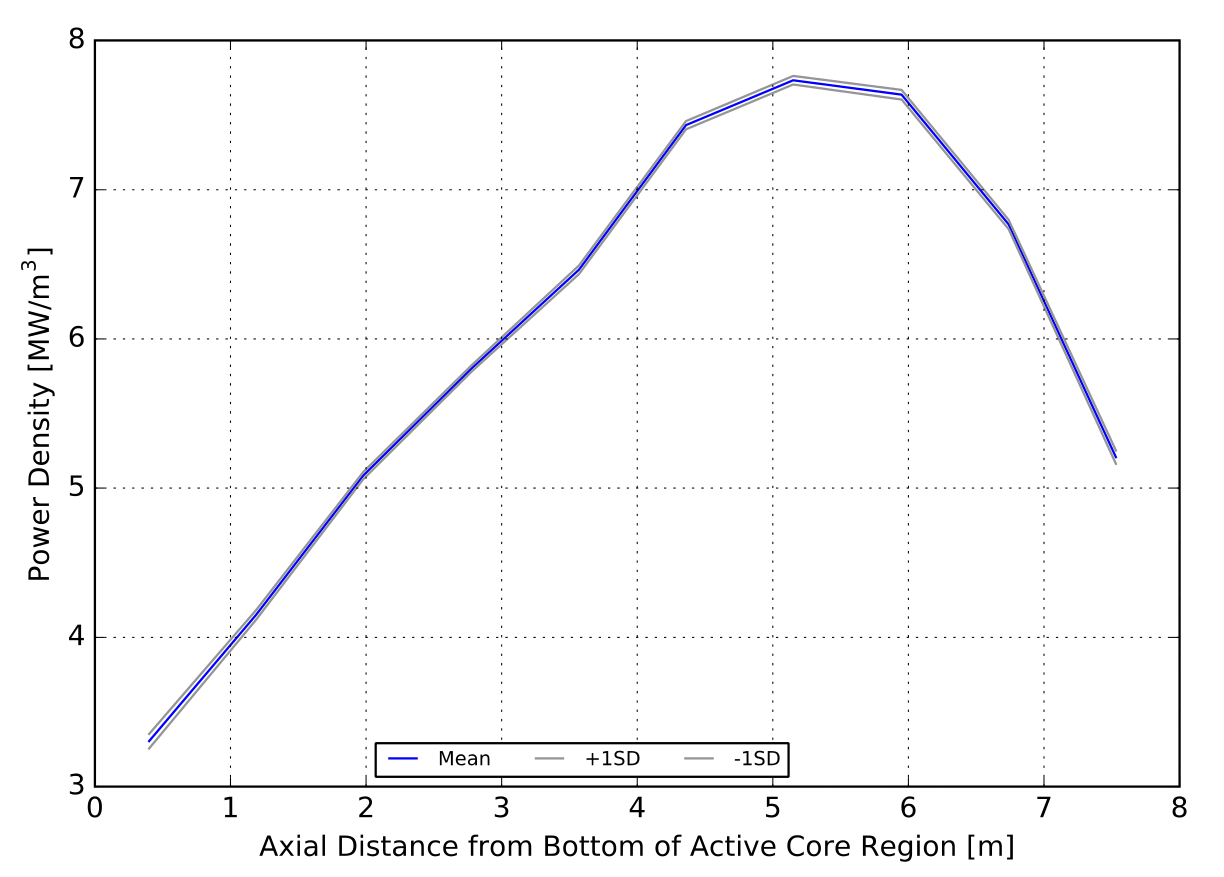
\includegraphics[width=0.47\textwidth]{figures-benchmark/benchmark-axialpower}
    }
	\hfill
	\caption{Radially averaged axial power distribution.}
	\label{fig:axialpower}
\end{figure}

\begin{figure}[htbp!]
	\centering
    \subfloat[Moltres result.]{
        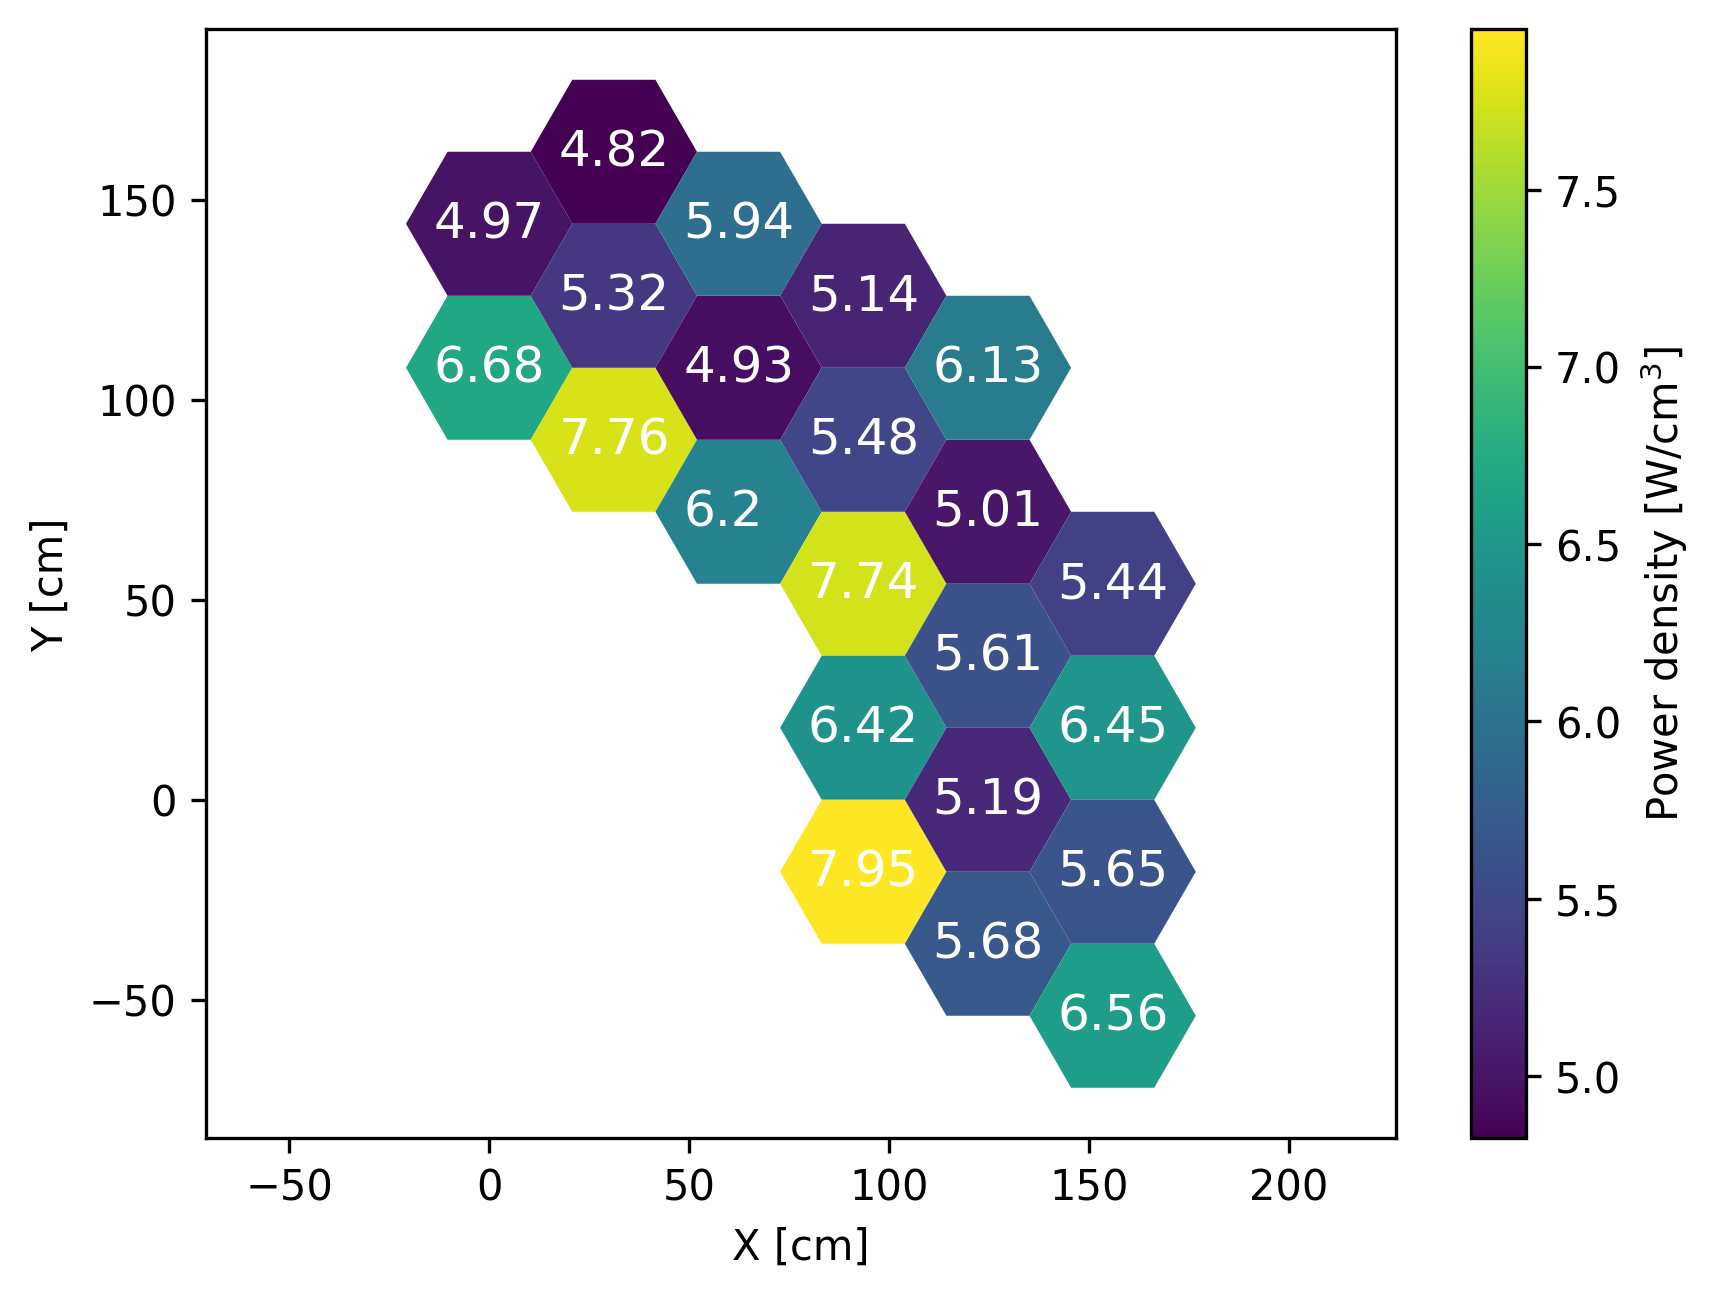
\includegraphics[width=0.47\textwidth]{figures-benchmark/3D-fullcore26G-radialpower}
    }
    \subfloat[Benchmark result. Image reproduced from \cite{oecd_nea_coupled_2020}.]{
        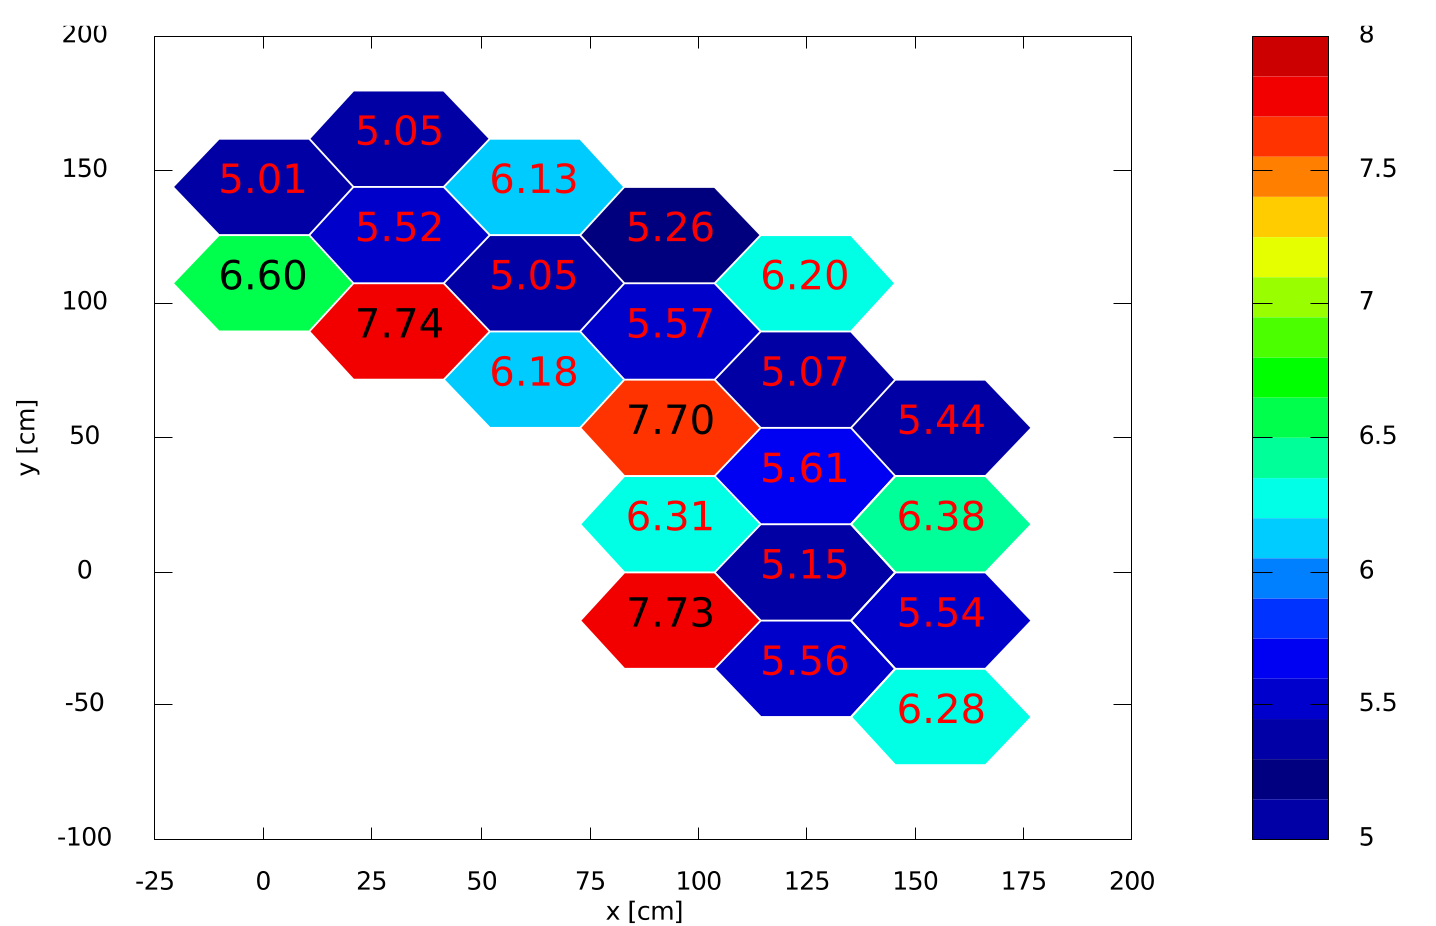
\includegraphics[width=0.42\textwidth, height=6.2cm]{figures-benchmark/benchmark-radialpower}
    }
	\hfill
  \caption{Axially averaged radial power distribution.}
  \label{fig:radialpower}
\end{figure}

\subsection{Periodic vs Reflective Boundary Conditions}
\label{sec:bench-bcs}

In the last section, we observed deviations in Moltres results.
In this section, we analyzed the discrepancies that the reflective \gls{BC} approximation may introduce.
As the previous section mentioned, the simulation's memory requirements restrict the use of periodic BCs.
To reduce the memory requirements, we collapsed the group constants to a smaller number of energy groups.
We simulated two cases: one that uses a 3-group structure and one that uses a 6-group structure (see Table \ref{tab:energygroups}).

The simulations required two meshes each, one for the CR out and one for the CR in.
The 3-group simulation had 62118 DoFs/energy-group (total of 186354 DoFs) and 61596 DoFs/energy-group (total of 184788 DoFs) for the CR out and CR in cases, respectively.
The 6-group simulation had 16898 DoFs/energy-group (total of 101388 DoFs) and 19116 DoFs/energy-group (total of 114696 DoFs) for the CR out and CR in cases, respectively.
We highlight that the 6-group simulation had to use a coarser mesh; otherwise, it would not run.
This fact confirms the suspicion that the simulation's memory requirements prevent it from running.

We ran simulations with periodic and reflective boundary conditions for both cases, and we compared their results.
Table \ref{tab:benchmark-bc} presents the results.
Keff rises with the reflective BC.
With the CR out, the raise is small.
However, with the CR in, the increase is considerable.
The combined effect of both increases leads to a decrease in the control rod worth.
The BC approximation barely affects the axial offset.

\begin{table}[htbp!]
  \centering
  \caption{Global parameters comparison for different types of BCs.}
  \begin{tabular}{l|l|l|l|l|l}
  \toprule
  Energy groups       & Type of BCs & K$_{eff, out}$ & K$_{eff, in}$ & $\Delta \rho_{CR}$ [pcm] & AO \\
  \midrule
  \multirow{2}{*}{3}  & Periodic     & 1.07571		& 1.06776		& 692.6		& 0.237		\\
                      & Reflective   & 1.07586	  & 1.07021   & 490.5		& 0.237	  \\ \hline
  \multirow{2}{*}{6}  & Periodic     & 1.07182		& 1.06356		& 724.3	  & 0.185  	\\
                      & Reflective   & 1.07197   	& 1.06610 	& 513.3		& 0.186		\\  
  \bottomrule
  \end{tabular}
  \label{tab:benchmark-bc}
\end{table}

\section{Conclusions}

% Preliminary studies: homogeneous vs heterogeneous isotopic distribution
The preliminary studies focused on several aspects of the simulations.
The first aspect was the effect of distributing the fuel compact isotopes homogeneously in the Serpent model.
The results showed that the homogenization of the fuel compact isotopes decreased the multiplication factor considerably.
The heterogeneous calculation took 28$\%$ more time.
Additionally, the homogeneous distribution appeared not to have a substantial impact on the group constants.
However, the multiplication factor's considerable difference suggested that the group constants’ small variations combined effect was significant.
Although the particles’ explicit modeling is time-consuming, it results necessary.

% Preliminary studies: homogeneous vs heterogeneous diffusion simulation
The next section studied the problem set-up in Moltres.
Different types of reactor technologies allow for homogeneous and heterogeneous diffusion calculations.
Moltres uses a heterogeneous diffusion solver.
In this work, we aim to use Moltres to solve prismatic HTGRs.
Nevertheless, the diffusion approximation fails to model properly regions where the mean free path is comparable to the region's dimensions.
The presence of helium in the fuel assembly of a prismatic \gls{HTGR} prohibits heterogeneous diffusion calculations.
Based on this discussion, we chose to use Moltres as a homogeneous diffusion solver.

% Serpent-Moltres: Fuel column
Focusing on a fuel column of the MHTGR-350, we investigated the effects of the energy group structure on the diffusion calculations.
We considered four different operational cases: a fuel column without LBPs and a fuel column with LBPs, both cases at 600K and 1200K.
Serpent obtained the homogenized group constants of the fuel column.
Moltres took such constants as input with a Gmsh mesh.
The first study compared the Moltres axial flux to Serpent axial flux.
Moltres used a 26 energy group structure to run the simulations.
Overall, the axial fluxes were close in shape and magnitude.
A different study focused on the effects of the energy group structure on the \gls{Keff}.
The number of energy groups did not affect the accuracy of the Moltres eigenvalue calculations.
We also compared the $L_2$-norm of the axial flux relative error in the active core using different energy group structures.
For the four operational cases, increasing the number of energy groups improved the accuracy
Additionally, we presented the simulation's computational expense for the different number of energy groups.
The simulation time and memory requirement rose by increasing the number of energy groups.
The computational time increased as well for the fuel column with LBPs.
Finally, we analyzed the impact of using different 15-group structures on the $L_2$-norm of the axial flux relative error.
We chose $15d$ as the best-performing energy group structure.

% Serpent-Moltres: Full-core
Based on the fuel column analysis results, we compared Moltres full-core results with Serpent reference results.
We considered two operational cases: 600K and 1200K.
Serpent obtained the homogenized group constants of the different regions of the reactor.
Moltres took such constants as input with a Gmsh mesh.
The first analysis compared the Serpent and Moltres eigenvalues.
Moltres results were bigger.
The overall differences were less than 300 pcm.
The second analysis compared the radial power distributions from both codes.
These results showcased the symmetry of the problem.
Reducing the problem size by half other simulations could reduce the computational expense.
For the most part, Moltres radial power distribution showed proximity to the Serpent's result.
We also compared Moltres and Serpent fluxes in two directions (axial and radial) in arbitrary core regions.
The axial fluxes showed small discrepancies, mostly in their magnitude.
The radial fluxes were close in shape and magnitude.
However, the radial flux in the diffusion calculation failed to capture the flux variation near the LBPs.
Overall, the fluxes were similar.

% OECD-Benchmark
The simulation capabilities for prismatic HTGRs have not reached the state of the art of LWRs.
This development delay motivated OECD/NEA to define a benchmark to carry out code-to-code comparisons.
The benchmark uses the MHTGR-350 as the reference design.
We conducted Phase I Exercise 1 with Moltres.
The benchmark defines the group constants for the exercise.
The group constants have a 26-energy group structure.
The benchmark exercise sets periodic \glspl{BC} on the sides of the geometry.
The simulation high memory requirements have challenged such implementation in Moltres. 
To go around such a barrier, we approximated the periodic \gls{BC} with a reflective BC.
Two out of three global parameters exhibited good agreement with the reference results.
However, the control rod worth presented a large discrepancy.
Such a difference was a consequence of the BC approximation.
Reducing the problem's size by collapsing the group constants to 3 and 6-energy groups, we compared the \gls{Keff} using the periodic and reflective BCs.
A reflective BC for the \gls{CR} out case did not substantially impact the \gls{Keff}.
On the other hand, the BC choice for the CR in case had a significant effect.
The combined effect of the approximation led to a large error in the CR worth.
The BC approximation had a small influence on the axial offset.